\chapter{涵道风扇式无人机的系统建模与硬件设计}
%第二章:涵道风扇式无人机的系统建模与硬件设计。首先定义了DFUAV的坐标系和姿态表示方法,然后采用牛顿-欧拉方法推导出DFUAV的刚体运动学模型和刚体动力学模型,并分析了作用在涵道上的力与力矩。%最后介绍了DFUAV的硬件设计,包括传感器、执行器等。

本章的重点是对如图\Ref{DFUAV}所示的DFUAV进行系统建模,这将是后续进行控制器设计的基础。物体的相对运动离不开其所处的参考坐标系,因此本章将先介绍本文所使用的多坐标系描述方法以及姿态表示方法。然后采用应用广泛的牛顿-欧拉方法推导出DFUAV的刚体运动学模型和动力学模型,得到飞行控制的刚体模型。最后分析了作用在涵道上的力与力矩。%最后介绍了DFUAV的硬件设计,包括传感器、执行器等。

DFUAV的系统建模中各变量定义标准主要参考文献\parencite{杨一栋2019直升机飞行控制},并为了表示方便,避免混淆,对部分变量的表示作略微修改。
\begin{figure}[htbp]
	\centering
	\begin{minipage}[c]{1\textwidth} % minipage将页面划分为0.5\textwidth
		\centering
		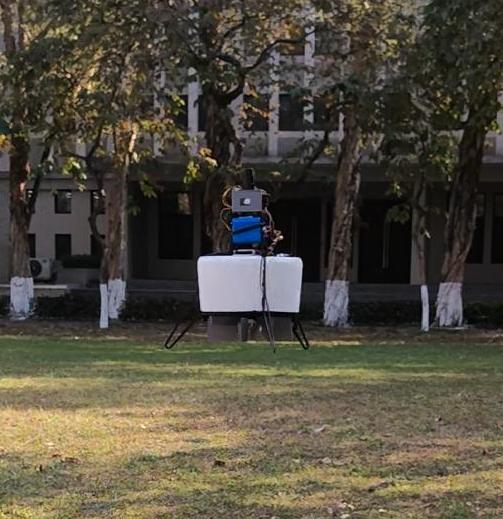
\includegraphics[scale=1]{Fig/DFUAV.jpg}
		\caption{\label{DFUAV}本文研究所使用的DFUAV}
	\end{minipage}%
\end{figure}

\section{坐标系和姿态表示方法}

在无人机领域,考虑到无人机的位置变化与姿态变化,基于地面坐标系($\boldsymbol{O}_e-\boldsymbol{X}_e\boldsymbol{Y}_e\boldsymbol{Z}_e $)和机体坐标系(${\boldsymbol{O}_b}-{\boldsymbol{X}_b}{\boldsymbol{Y}_b}{\boldsymbol{Z}_b}$)的多坐标系表示法被广泛采用。如图\ref{坐标系}所示。

\begin{figure}[htbp]
	\centering
	\begin{minipage}[c]{1\textwidth}
		\centering
		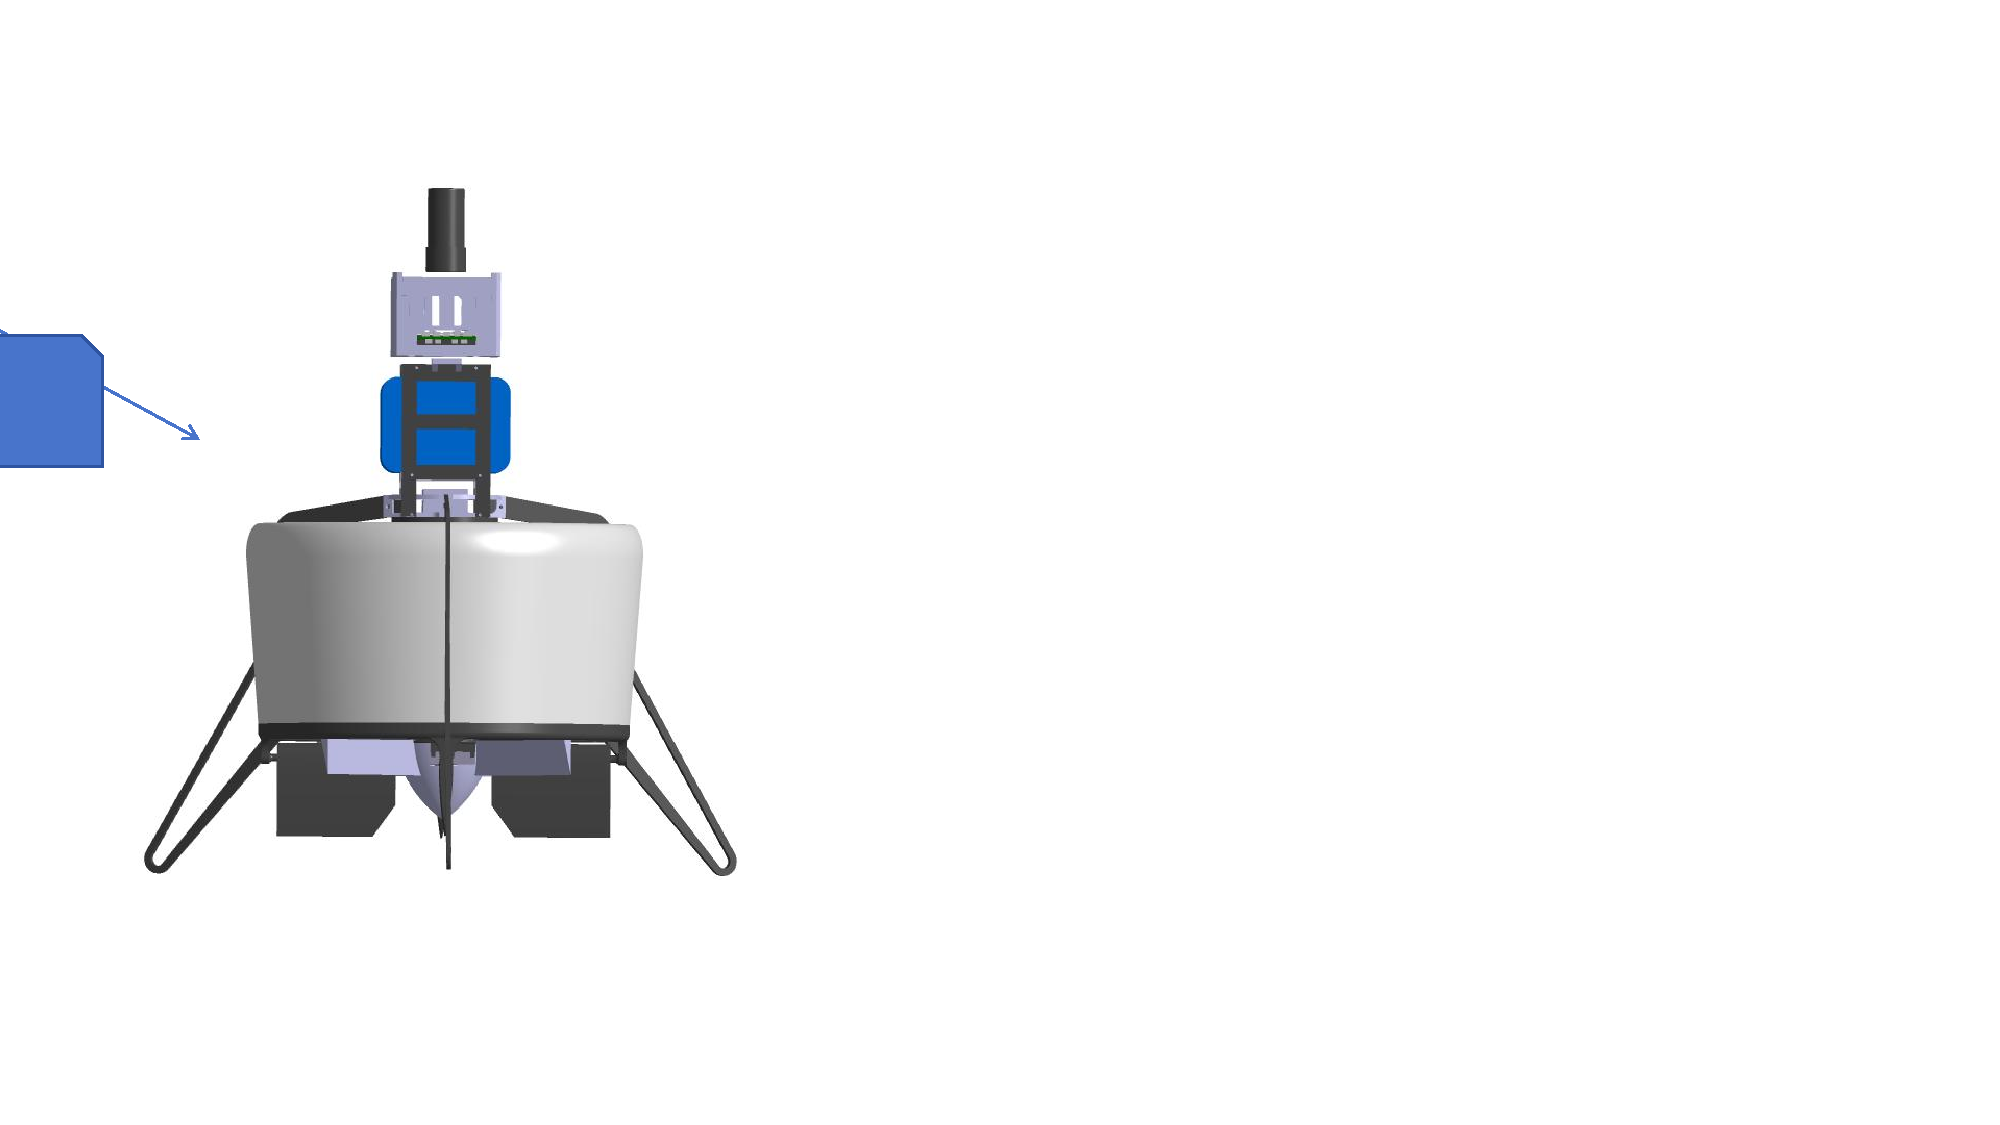
\includegraphics[scale=1]{Fig/演示文稿1.pdf}
		\caption{\label{坐标系}地面坐标系与机体坐标系示意}
	\end{minipage}%
\end{figure}









与很多外文杂志社不同,大部分中文期刊都不提供\LaTeX{}模板给投稿者使用,也很少有学校给学生提供官方的毕业论文模板。目前github上的大部分模板都是由学生发起的非官方模板。在此感谢Shun Xu以及yecfly等人的工作,他们的无私贡献使得华南理工大学硕博士毕业论文也可以使用\LaTeX{}撰写。

本模板是直接修改前人的模板得到的,更详细的介绍可到\parencite{_,_a}下载。本章仅从用户的角度简要介绍模板的使用,而尽量避免涉及\LaTeX{}的模板制作细节(实际上是因为本人也不会)。正如我们使用手机并不需要了解麦克斯韦方程组,使用\LaTeX{}写作也无需了解模板是如何制作的。

\LaTeX{}的源代码保存在后缀名为.tex的文件中。当编写长篇文档时,例如当编写书籍、毕业论文时,单个源文件会使修改、校对变得十分困
难。将源文件分割成若干个文件,例如将每章内容单独写在一个文件中,会大大简化修改和校对
的工作。为方便,本文将scutthesis.tex文件称为主文件,而将chapter文件夹的abstract.tex、chapter0x.tex、conclusion.tex等文件称为章节文件。

值得注意的是,要每次编译时都更新参考文献著录,TeXstudio软件的选项->设置中的构建并查看、编译器需要设置成如图\ref{TeXstudio}、\ref{setup}所示。此时只需在任意一个文件中点击构建并查看按钮即可编译文档。每次编译都更新参考文献会使得编译时间很长。
\begin{figure}[htbp]
	\centering
	\includegraphics[scale=0.55]{Fig/TeXstudio.png}
	\caption{\label{TeXstudio}TeXstudio环境}
\end{figure}
\begin{figure}[htbp]
	\centering
	\includegraphics[scale=0.55]{Fig/setup.png}
	\caption{\label{setup}TeXstudio编译选项}
\end{figure}

\section{主文件}
scutthesis.tex文件相当于主函数,调用各章的内容。\LaTeX{}源代码以一个\textbackslash{}documentclass 命令作为开头,它指定了文档使用的文档类。文档类规定了\LaTeX{}源代码所要生成的文档的性质——普通文章、书籍、演示文稿、个人简
历等等。
\begin{lstlisting}
\documentclass[<options>]{<class-name>}
\end{lstlisting}
其中class-name为文档类的名称,如\LaTeX{}提供的article, book, report,可在其基础上派
生的一些文档类或者有其它功能的一些文档类。\LaTeX{}提供的基础文档类见文献\parencite{_c}。还可以自定义文档类,如华南理工大学硕博士论文文档类scutthesis,其实现保存在后缀名为.cls的文件中。可选参数options 为文档类指定选项。


document环境当中的内容是文档正文:
\begin{lstlisting}
\begin{document}
正文内容
\end{document}
\end{lstlisting}
正文中包含各章节内容:
\begin{lstlisting}
\chapter{摘\texorpdfstring{\quad}{}要}
	本模板由Shun Xu\cite{_}以及yecfly\cite{_a}的模板修改而来,适合于华南理工大学硕/博士毕业论文。既然已经入坑LaTeX,就不推荐使用LYX,但本模板在修改祖传代码过程中仅对修改部分进行更新,其余部分仍保留源代码。另外参考文献管理软件推荐使用zotero,这也是本模板使用的软件。本模板最主要的改动是参考文献使用biber,而不是原来的bibtex,因此不再需要.bst文件。

\keywordsCN{\LaTeX{};论文}

\chapter{Abstract}
	

\keywordsEN{\LaTeX{}; Paper} % 中英文摘要
\tableofcontents	% 目录
\listoftables	% 表格目录(可选)
\listoffigures	% 插图目录(可选)
\chapter{主要符号对照表}

\begin{table}
	\centering{}%
	\begin{tabular}{l>{\centering}p{0.5cm}l}
	 $ \boldsymbol{O}_e-\boldsymbol{X}_e\boldsymbol{Y}_e\boldsymbol{Z}_e $-地面坐标系  &  & ${\boldsymbol{O}_b}-{\boldsymbol{X}_b}{\boldsymbol{Y}_b}{\boldsymbol{Z}_b}$-机体坐标系\tabularnewline
     $\boldsymbol{P}^{e}=\begin{bmatrix}{x}^{e}&{y}^{e}&{z}^{e}\end{bmatrix}^{T}$-无人机在地面坐标系下的位置 &  & $\boldsymbol{V}^{e}=\begin{bmatrix}{v}^{e}_{x}&{v}^{e}_{y}&{v}^{e}_{z}\end{bmatrix}^{T}$-无人机在地面坐标系下的速度\tabularnewline
     $\boldsymbol{V}^{b}=\begin{bmatrix}{u}&{v}&{w}\end{bmatrix}^{T}$-无人机在机体坐标系下的速度 && $ \psi $-偏航角\tabularnewline
	 $\theta$-俯仰角 && $\varphi$-滚转角\tabularnewline
	 $\boldsymbol{R}^n_b$、$\boldsymbol{R}$-机体系到NED系的旋转矩阵\tabularnewline
	 $\boldsymbol{G}$-NED系的重力  							  &  &   $\varphi_0 $-气动面安装角\tabularnewline
	 $ w $-系统的外部扰动								&  &  $T$-系统采样周期\tabularnewline
	 $\boldsymbol{F}$-机体系的气动力 						    &  &   $\boldsymbol{M}$-机体系的气动力矩\tabularnewline
	 $\rho$-空气密度 								  &  &  $C_{D,x} $、$ C_{D,y} $、$ C_{D,z} $-沿机体轴阻力系数\tabularnewline
	 $A_x $、$ A_y $、$ A_z $-沿机体轴的截面面积 		 &  &  $v$-机身相对于空气的速度分量\tabularnewline 
	 $l_{a}$-机身气动阻力作用点与重心的距离   			  &  &  $V_c$-气体在无穷远处的速度\tabularnewline
	 $T_d$-涵道体升力  								 &  &  $T_p$-风扇升力\tabularnewline
	 $T_a$-总升力 								      &  &  $q_a$-涵道升力分配系数\tabularnewline
	 $ p_U $-桨盘上表面压强 						   &  &  $p_L$-桨盘下表面压强\tabularnewline
	 $V_c+V_i$-桨盘上下表面气体速度 					 &  &  $S$-桨盘面积\tabularnewline
	 $ V_i $-桨盘处气流诱导速度 						  &  &  $ V_{cr} $-理想自转下降速率\tabularnewline
	 $ Q $-风扇扭矩 								 &  &  $ \varpi $-风扇转速\tabularnewline
	 $\mu$-环绕涵道角度变量 						  &  &  $\hat{\boldsymbol{i}}$-沿机体系$x$轴方向的单位矢量\tabularnewline 
	 $\hat{\boldsymbol{j}}$-沿机体系$y$轴方向的单位矢量  	   &  &  $C_{l, d}(\alpha_d)$-涵道翼型升力曲线\tabularnewline 
	 $C_{d, d}(\alpha_d)$涵道翼型阻力曲线  		      &  &  $c_d$-涵道翼型弦长\tabularnewline 
	 $C_{l_{\alpha}}$-风管翼型升力曲线斜率  			 &  &  $C_{l, \min }$、$ C_{l, \max } $-升力系数极限\tabularnewline 
	 $C_{d, o }$、$C_{d, g }$-拟合阻力曲线经验常数 	&  &  $R$-风扇半径\tabularnewline 
	 $C_{d u c t}$ - 常值比例系数  					&  &  $l_{d}$-重心与涵道气动力作用点的距离\tabularnewline
	 $k_{\delta}$-操纵面气动升力系数 				 &  &  $\alpha_d$-攻角\tabularnewline
	 $ I_{b}$-风扇转动惯量  						   &  &  $ d_{af} $ 、$ d_{ds} $-风扇扭矩常系数\tabularnewline
	 $\boldsymbol{L}_{{r}}$-风扇角动量  						&  & \tabularnewline 					
	\end{tabular}
\end{table}	% 符号对照表(可选)
\chapter{英文缩略词}
【本节论文规范为可选,如果你的论文没有相关内容那么去除这一节;如果有,则删除这一行注释。】
\begin{table}
	\centering{}%
	\begin{tabular}{ccc}
		SCUT  & South China University of Technology & 华南理工大学\tabularnewline
		&  & \tabularnewline
		&  & \tabularnewline
		&  & \tabularnewline
		&  & \tabularnewline
	\end{tabular}
\end{table} 	% 缩略词	
...
\chapter{绪论}
%
\section{研究背景和意义}
% \subsection{研究背景和意义}
%
2010年,我国正式提出“低空经济”这一概念。2024年也被称为低空经济元年,全国两会首次将“低空经济”写入政府工作报告中。无人机(Unmanned Aerial Vehicle,UAV)作为低空经济这一战略新兴产业的重要形态之一,近些年来发展得如火如荼,已经在军事、民用、科研等领域得到了广泛应用。顾名思义,无人机是一种不需要飞行员在飞机上驾驶的飞行器,它的飞行控制可以由飞行员在地面的控制站上进行操纵,也可以基于事先设计好的轨迹完全自主飞行,或者借助如人工智能(Artificial Intelligence,AI)等先进技术在复杂环境中实时地规划轨迹来避障飞行\cite{rezwanArtificialIntelligenceApproaches2022}。

无人机最早于第一次世界大战期间被研制出来用于军事对抗。受限于二十世纪初的科学技术条件,当时的无人机并没有在战场上发挥很大的作用,但是人们并没有因此停止对无人机的研究与发展。时至今日,无人机在俄乌战争中被大规模使用,主要用来执行目标搜寻、侦察、打击和救援等任务,深刻地影响了战场局势。在2022年的最后一个晚上,乌克兰的四旋翼无人机向俄罗斯士兵投下了小型炸弹,其凭借着机载的热成像系统实现了在漆黑的夜晚对俄罗斯士兵进行准确打击\cite{kunertovaWarUkraineShows2023}。无独有偶,由俄罗斯Kronshtadt公司开发的“猎户座(Orion)”固定翼无人机(见图\ref{Orion})也已成功用于攻击乌克兰阵地。该无人机前部安装了一个可以转动的炮塔系统,内部装有红外传感器和激光雷达等设备,用于引导高精武器准确打击目标。除军事用途外,无人机也在民用领域大展身手。例如,无人机结合人工智能以及机器学习(Machine Learning,ML)方法,通过提升效率、环境可持续性和数据驱动的决策指定,为精准农业带来了重大革新\cite{agrawal2024transforming}。2022年,意大利Cristiano Fragassa教授团队利用无人机从不同的飞行高度拍摄杂草丛生的田地的图像,开发和测试了一种机器学习方法用来识别植被斑块。该方法可以精确地识别出整个大规模耕作田中的农作物和杂草,该信息可以用来帮助减少水、肥料和除草剂的使用\cite{fragassaNewProcedureCombining2023}。在国内,以大疆创新和极飞科技等为代表的科技公司都有自研的农业无人机产品。以极飞P150PRO 2025款农业无人机为例(见图\ref{P150PRO}),该无人机集农药喷洒、种子播撒、货物运输和航拍测绘多种功能为一体,每分钟最大喷洒流量可达32升,单次航测面积最大可达300亩。科研院校中如中国农业大学、华南农业大学\cite{liuAgriculturalUAVObstacle2024a}等也都在农业无人机方面取得研究进展。

\begin{figure}[htbp]
	\centering
	\begin{minipage}[c]{0.5\textwidth} % minipage将页面划分为0.5\textwidth
		\centering
		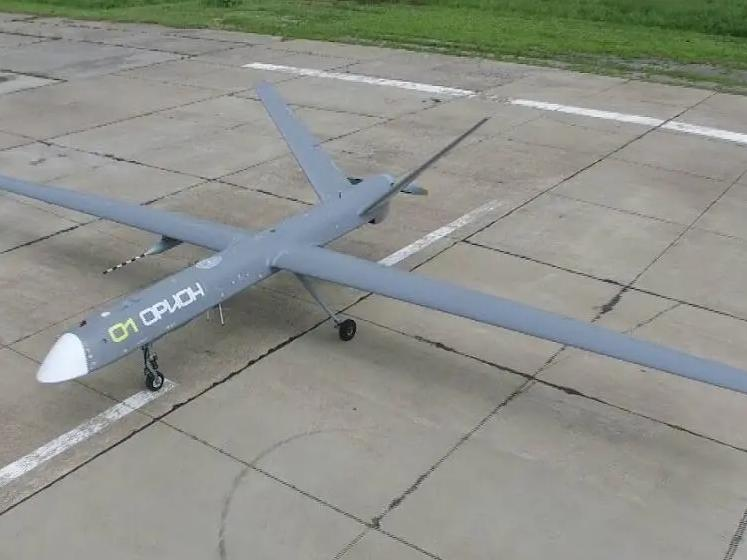
\includegraphics[width=6cm,height=5cm]{Fig/Orion.jpg}
		\caption{\label{Orion}猎户座固定翼无人机}
	\end{minipage}%
	\begin{minipage}[c]{0.5\textwidth}
		\centering
		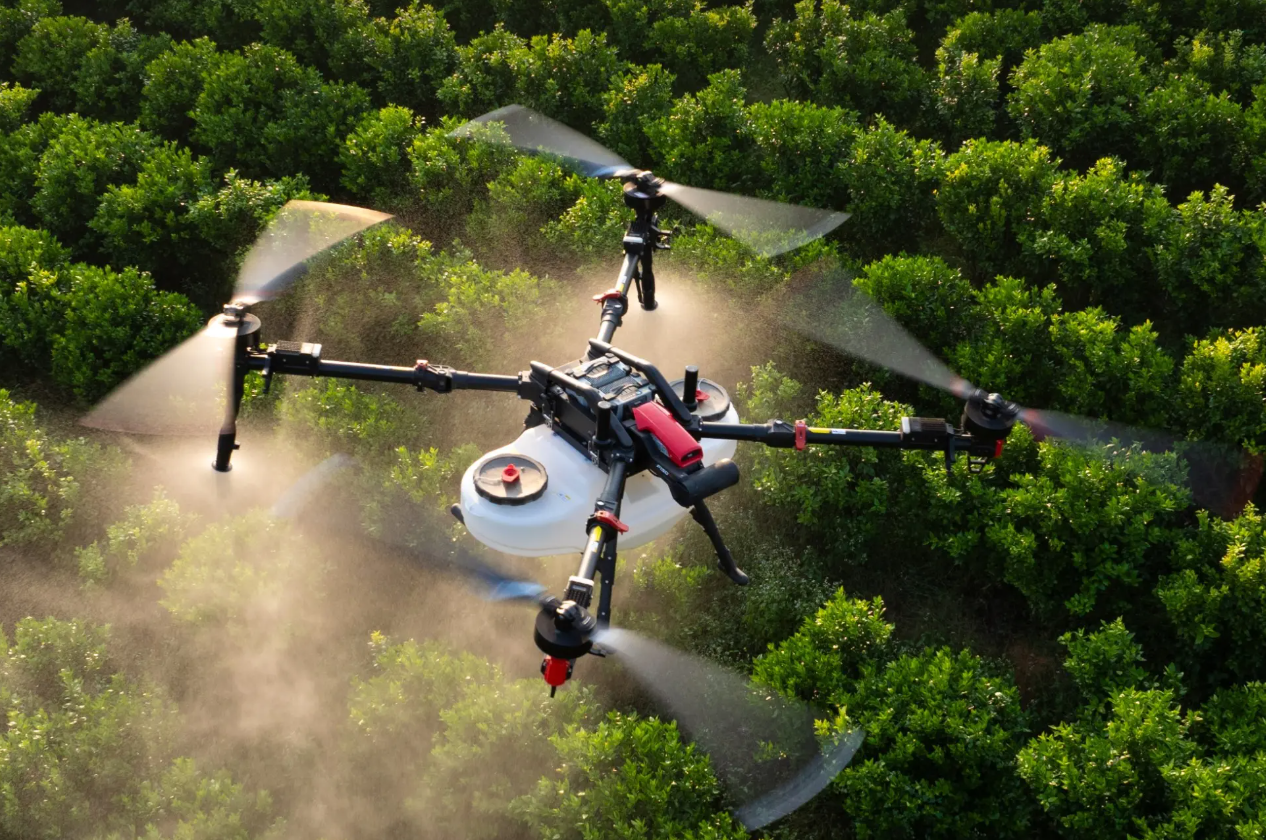
\includegraphics[width=6cm,height=5cm]{Fig/P150PRO.png}
		\caption{\label{P150PRO}极飞P150PRO农业无人机}
	\end{minipage}
\end{figure}

无人机发展百年,种类繁多,不同的任务需求驱动着创造不同类型的无人机。因此按照无人机的任务能力,可将其分为水平起飞着陆(Horizontal Take-off Landing,HTOL)、垂直起飞着陆(Vertical Take-off Landing,VTOL)、混合模型(倾转翼、倾转旋翼和涵道风扇)、直升机和非常规类型\cite{hassanalianClassificationsApplicationsDesign2017}。其中,涵道风扇无人机(Ducted Fan UAV,DFUAV)是指其螺旋桨被封闭在涵道内部的无人机,这些螺旋桨也被称为“风扇”,同时下方安装有若干控制舵面进行控制。DFUAV既有旋翼无人机般的垂直起降能力,又可以像固定翼无人机那样高速巡航,而且这种特殊的配置结构具有空气动力效率高和操作安全性的优势\cite{johnsonModelingControlFlight2006b,zhangReviewDuctedFans2020b,qianImprovingPerformanceDucted2022}。但不如人意的是,与开放旋翼相比,涵道风扇的罩状旋翼在飞行器周围的流场中会表现出强烈的耦合效应\cite{iiiNondimensionalModelingDuctedFan2012},并且由于其特殊的气动布局,DFUAV在垂直起降和水平巡航这两种不同的飞行模式下气动特性也完全不同\cite{johnsonModelingControlFlight2006b},这都对DFUAV的控制器设计提出了挑战。此外,针对DFUAV的轨迹规划的研究相对匮乏,这种研究的不足在一定程度上限制了DFUAV在复杂环境中的高效运作,不利于DFUAV的进一步推广应用。

正因如此,设计出适用于DFUAV的控制策略以及合理的轨迹规划方法,对于DFUAV的进一步发展具有重要意义。

\section{国内外研究现状}

\subsection{涵道风扇无人机}

目前已知的关于涵道风扇无人机的起源最早可以追溯到二十世纪三十年代,由意大利的Stipa和德国的Kort率先在该领域开展研究\cite{iiiNondimensionalModelingDuctedFan2012}。在二十世纪五十年代,美国宇航局在研究Doak VZ-4和Bell X-22涵道风扇垂直起降飞行器时投入了大量精力后取得一些进展,然而他们也发现了一些意料之外的特性,如从悬停到前飞过渡时,会出现机头上仰的趋势\cite{cookSummaryLiftLift1993}。Pereira等人\cite{pereiraHoverWindtunnelTesting2008}已经对涵道风扇早期的研究进行了详尽的回顾。近年来,随着先进的控制方法的提出和涵道风扇理论的进一步完善,涵道风扇无人机这一领域不仅引起了众多科研机构的广泛关注,还催生出了一系列具有里程碑意义的创新产品。

在二十世纪八十年代末期,美国Sikorsky航空公司试飞了一种名为“Cypher”的小型无人机。该无人机涵道直径1.75m,重量为20kg,采用共轴双桨结构提供动力,环形护罩在提升了拉力效率的同时也提升了其安全性。1992年4月,在初代Cypher的基础上,Cypher II进行了首次飞行。相比初代Cypher,Cypher II涵道直径1.9m,重量为110kg,并且在环形护罩外扩展了固定翼结构,并且尾部还有一个推进式螺旋桨,有效提升了Cypher II的飞行速度以及续航时间\cite{murphy1996air},最高时速可达230km/h,航程超过185km。

\begin{figure}[htbp]
	\centering
	\begin{minipage}[c]{0.5\textwidth} % minipage将页面划分为0.5\textwidth
		\centering
		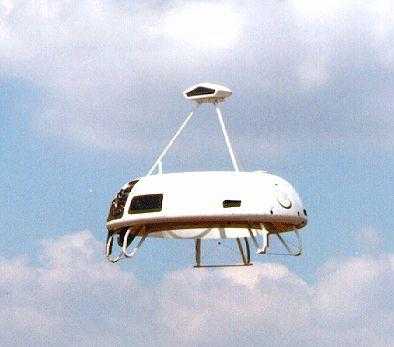
\includegraphics[width=6cm,height=5cm]{Fig/Cypher.jpg}
		\caption{\label{Cypher}Cypher}
	\end{minipage}%
	\begin{minipage}[c]{0.5\textwidth}
		\centering
		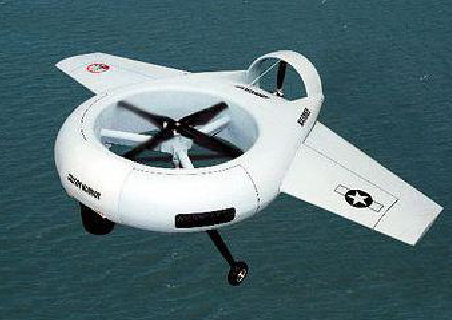
\includegraphics[width=6cm,height=5cm]{Fig/Cypher II.png}
		\caption{\label{Cypher II}Cypher II}
	\end{minipage}
\end{figure}

2003年,美国极光飞行科技公司根据国防高级研究计划局的“秘密无人机”计划开发了GoldenEye-100无人机,可垂直起降并且能携带11kg的有效载荷。次年7月,由GoldenEye-100衍生出的更小的GoldenEye-50无人机首飞。GoldenEye-50长70cm,翼展1.4m,最大飞行速度可达280km/h\cite{schaeferGoldenEyeClandestineUAV},并且在2005年4月进行了第一次自主水平飞行转换。GoldenEye-80是GoldenEye系列的第三个版本,长165cm,重达68kg,携带有高分辨率摄像机和激光测距仪等传感设备,设计意图用于满足美国陆军未来作战系统计划的要求。

2003年,Honeywell航空航天公司为美国陆军开发制造了RQ-16 T-Hawk微型无人机,并于2007年部署在了伊拉克战场上\cite{white2010upgrades}。该款无人机采用涵道风扇设计,涵道直径为35.5cm,总机重量为7.7kg,巡航速度可达74km/h,在战场上被广泛应用于可疑目标检查和跟随等任务。在2011年日本地震引发海啸进而导致核泄露后,4架T-Hawk被部署在福岛1号核电站,其机载的高分辨率摄像头拍摄了核电站受损部分的图像用于帮助日本核工程专家快速定位和解决问题。但是后来有两架T-Hawk在核反应堆上空坠毁,Honeywell公司并没有给出具体原因。

\begin{figure}[htbp]
	\centering
	\begin{minipage}[c]{0.5\textwidth} % minipage将页面划分为0.5\textwidth
		\centering
		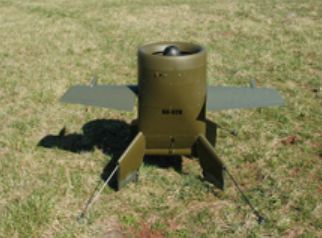
\includegraphics[width=6cm,height=5cm]{Fig/GoldenEye.png}
		\caption{\label{GoldenEye}GoldenEye}
	\end{minipage}%
	\begin{minipage}[c]{0.5\textwidth}
		\centering
		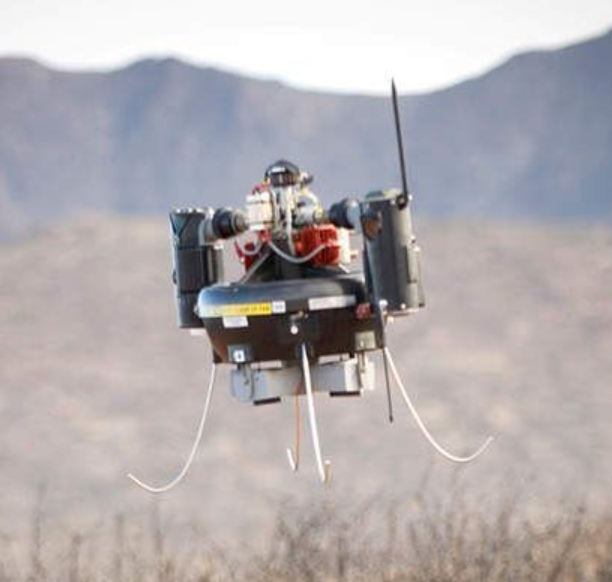
\includegraphics[width=6cm,height=5cm]{Fig/T-Hawk.png}
		\caption{\label{T-Hawk}T-Hawk}
	\end{minipage}
\end{figure}

2015年12月30日,由以色列Tactical Robotics公司研发的AirMule救护无人机首航。如图所示,AirMule的起飞旋翼设置在了机身内部,由涵道壁包裹,尾部还有两个推进涵道风扇用于控制姿态。这种构型专为直升机不方便起降的情形而设计,如山川、林地等地形复杂的区域。由于AirMule可负载80kg的载重能力和150km/h的最大速度\cite{yuTechnicalAnalysisVTOL2016},未来还将用于运输货物等任务。

\begin{figure}[htbp]
	\centering
	\begin{minipage}[c]{0.5\textwidth} % minipage将页面划分为0.5\textwidth
		\centering
		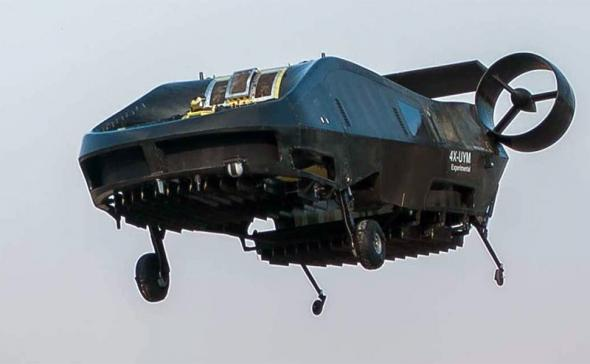
\includegraphics[width=7cm,height=5cm]{Fig/AirMule.jpg}
		\caption{\label{AirMule}AirMule}
	\end{minipage}%
	\begin{minipage}[c]{0.5\textwidth}
		\centering
		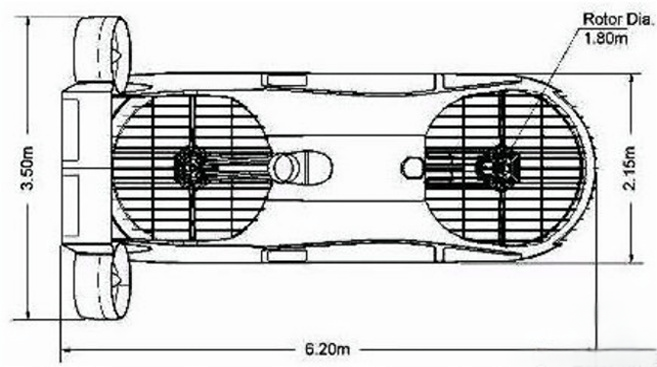
\includegraphics[width=7cm,height=5cm]{Fig/Airmule内部结构.png}
		\caption{\label{AirMule2}Airmule内部结构}
	\end{minipage}
\end{figure}

在2016年的HWTrek全球智能硬件创新与制造大会上,来自比利时无人机Fleye引发众人关注,如图所示。因其大小与篮球相当,许多媒体也把它称为“球形无人机”。Fleye也属于涵道风扇无人机的一种,摄像头安装在上部,下部为光流传感器,由于其安全小巧的特点,媒体预测其未来将会应用于室内摄影、娱乐等场合。除上述提到的采用涵道构型无人机外,还有由新加坡ST Aerospace研发的FanTail系列\cite{mateosanguinoDesignStabilizationCoanda2024}、Aesir公司的Odin\cite{crivoi2013survey}和美国联合宇航公司的iSTAR\cite{flemingImprovingControlSystem}等。

\begin{figure}[htbp]
	\centering
	\begin{minipage}[c]{0.33\textwidth} % minipage将页面划分为0.5\textwidth
		\centering
		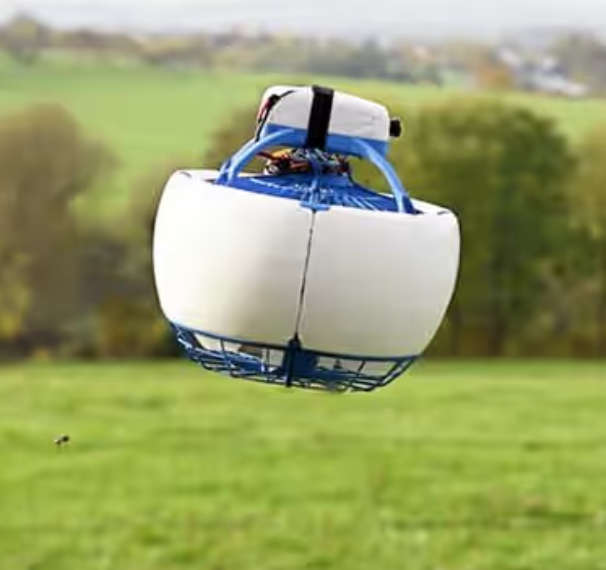
\includegraphics[width=5cm,height=5cm]{Fig/Fleye.png}
		\caption{\label{Fleye}Fleye}
	\end{minipage}%
	\begin{minipage}[c]{0.33\textwidth}
		\centering
		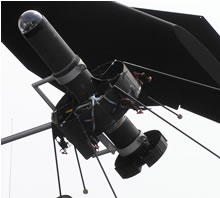
\includegraphics[width=5cm,height=5cm]{Fig/FanTail.png}
		\caption{\label{FanTail}FanTail}
	\end{minipage}
    \begin{minipage}[c]{0.33\textwidth}
		\centering
		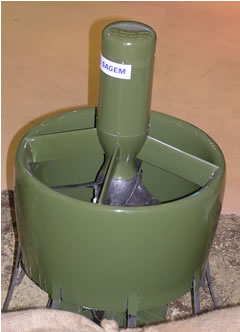
\includegraphics[width=4cm,height=5cm]{Fig/odin.jpg}
		\caption{\label{odin}Odin}
	\end{minipage}
\end{figure}

相较于国外的研究成果,我国涵道无人机研究起步相对较晚,大多处于实验探索阶段。2008年,哈尔滨盛世特种飞行器有限公司与中国航天科工集团第四研究院和哈尔滨工业大学航天学院合作共同研发制造出国内首例单桨环道“飞碟”,直径1.2m,续航40分钟,最大速度可达80km/h,并获得国家发明专利。由南昌航空大学设计的“都市精灵”涵道无人机获得2011年“中航工业杯—国际无人飞行器创新大奖赛”创意奖,其涵道直径1.2m,续航时间1h,最大飞行速度为50km/h。深圳千叶智能科技公司以研发涵道式无人机设计平台为主,目前已推出CDF-270、CDF-390和EDF-254等型号的无人机,可用于航拍、巡航和侦察等领域。

\begin{figure}[htbp]
	\centering
	\begin{minipage}[c]{0.33\textwidth} % minipage将页面划分为0.5\textwidth
		\centering
		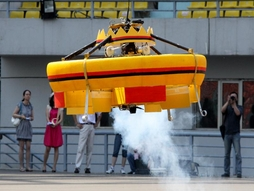
\includegraphics[width=5cm,height=5cm]{Fig/飞碟.jpg}
		\caption{\label{飞碟}飞碟}
	\end{minipage}%
	\begin{minipage}[c]{0.33\textwidth}
		\centering
		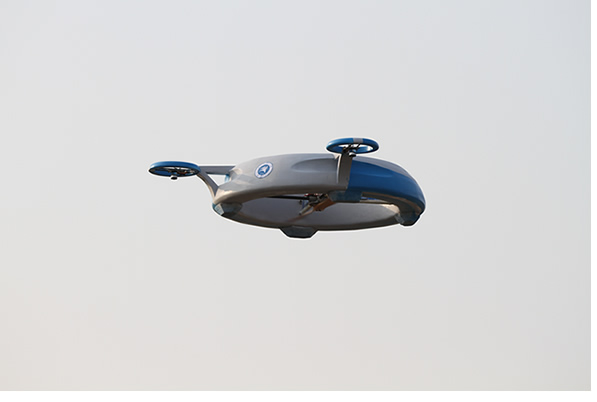
\includegraphics[width=5cm,height=5cm]{Fig/都市精灵.jpg}
		\caption{\label{都市精灵}都市精灵}
	\end{minipage}
    \begin{minipage}[c]{0.33\textwidth}
		\centering
		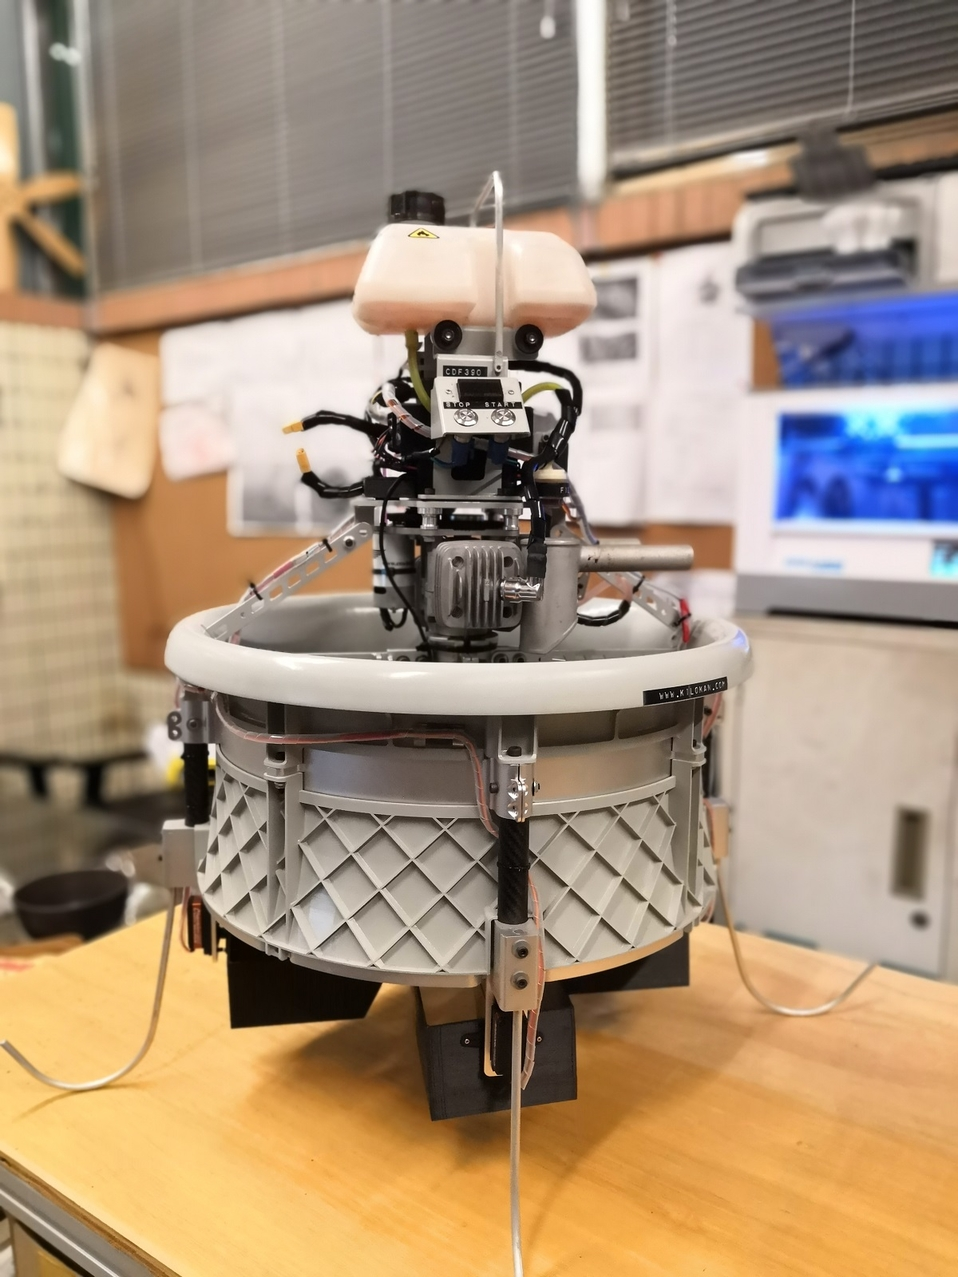
\includegraphics[width=4cm,height=5cm]{Fig/CDF-390.jpg}
		\caption{\label{CDF-390}CDF-390}
	\end{minipage}
\end{figure}

此外,清华大学\cite{chouStudyOverallDesign2021,luoNumericalAnalysisWind2024a}、北京理工大学\cite{manzoorCompoundLearningBasedModel2024}、南京航空航天大学\cite{caiNumericalPredictionUnsteady2022}和华南理工大学\cite{yinDuctedFanUAV2024,1022766347.nh}等高校也对涵道无人机展开了不同程度的研究,极大推动了我国在该领域的发展。

\subsection{飞行控制技术}

涵道风扇无人机的飞行控制技术是涵道风扇无人机研究的重要组成部分。飞行控制技术的研究主要包括控制器设计、轨迹规划和飞行仿真等方面。控制器设计是涵道风扇无人机飞行控制技服的核心,其目的是设计出一种能够使无人机在飞行过程中保持稳定的控制器。轨迹规划是指在给定的环境条件下,设计出一种使无人机能够按照预定的轨迹飞行的方法。飞行仿真是指利用计算机模拟无人机的飞行过程,以验证控制器设计和轨迹规划的有效性。

这里主要是想推荐一种“学术生态”,即利用各种工具展开科研工作,以达到事半功倍的效果。需要用到以下软件:
\begin{enumerate}[topsep = 0 pt, itemsep= 0 pt, parsep=0pt, partopsep=0pt, leftmargin=44pt, itemindent=0pt, labelsep=6pt, label=(\arabic*)]
	\item 	参考文献管理软件zotero\cite{_m}。很多人使用过endnote,但其实zotero也非常强大,强烈推荐。可到b站观看Struggle with Me出品的视频教程\cite{_k}入门(或其他最新教程,刚开始不推荐使用插件,会增加学习难度)。zotero自带pdf阅读器,也可以设置为使用其他阅读器。在zotero可以打开文件所在位置,故不推荐更改zotero的文件系统(尤其不推荐使用zotfile插件,事实上各种五花八门的插件增加了复杂性,实际上没有带来太多便利性)。理论上只需要包含文献元数据信息的bib文件(可以手动一篇一篇文章地收集)即可使用此模板,因此模板不依赖于任何参考文献管理软件,endnote用户或不使用参考文献管理软件的用户可以忽略本文zotero部分的讲解。
	\item	可截图获取文献中公式的软件mathpix\cite{_h}。在阅读别人的论文时,很可能需要把文章中的公式抄下来放到自己的笔记中,方便以后组会报告甚至论文中使用,这时使用mathpix可直接截图获取\LaTeX{}源码,非常方便。该软件普通邮箱注册可每月50次免费,学校邮箱可100次,若信用卡注册可1000次(最新情况是只能500次了,还要收费20美元,世界变化太快了)。注:随着mathpix的使用成本越来越高,免费次数越来越少,2023起已经不再推荐。目前开源/免费的替代工具为:。\href{https://www.simpletex.cn/}{SimpleTex}和\href{https://p2t.breezedeus.com/}{Pix2Tex}。目前SimpleTex性能比较好,免费但不开源,不排除未来收费的可能
	\item	TeXlive202x、TeXstudio,相当于开发环境和IDE。本模板是基于TeX的发行版TeXlive202x和编辑器TeXstudio进行的,百度这两个关键字分别安装。关于TeXstudio的使用(快捷键等)可另行查找资料。模板还支持更多ide,更多编译方式见GitHub首页readme.md。若在其他窗口打开了编译生成的pdf文件,记得关掉再编译,否则报错。TeXstudio的设置见第二章。
\end{enumerate}

本文的章节安排如下:

第一章,绪论。

第二章,模板简介。主要介绍各文件的内容。

第三章,常用环境。介绍论文写作中常用的环境,包括:图、表、公式、定理。基本涵盖了常用的命令。

%第三章,参考文献设置。本模板对旧版的改动主要是参考文献部分,本章将简单参考文献设置以及
%编译选项的设置等等。


	% 第一章
\chapter{涵道风扇式无人机系统构成及建模}

为方便检验本文的研究成果,自主搭建了一架DFUAV试验样机。本章首先简要介绍试验样机的结构组成和机载航电系统,然后重点是对DFUAV进行系统建模,这将是后续进行飞行控制算法设计的基础。物体的相对运动离不开其所处的参考坐标系,因此在建模之前将先介绍本文所使用的坐标系描述方法以及DFUAV的姿态表示方法。在建模分析中,为简化模型复杂度便于控制算法的设计,有必要假设无人机是刚体。然后采用在刚体上应用广泛的牛顿-欧拉方法推导出DFUAV的刚体运动学模型和动力学模型,得到飞行控制的刚体模型。最后分析了作用在涵道上的力与力矩并作出总结。
% DFUAV的系统建模中各变量定义标准主要参考文献\parencite{杨一栋2019直升机飞行控制},并为了表示方便,避免混淆,对部分变量的表示作略微修改。

\section{试验样机的系统组成}

\subsection{主要结构介绍}

自主搭建的DFUAV试验样机的实物及主要结构如图\ref{DFUAV}所示。类似大部分无人机,DFUAV也有电子仓、电池、电调、电机和螺旋桨等组成部件。电子仓中放置了飞行控制系统的硬件,电池是DFUAV的能量来源,电调、电机和螺旋桨共同组成了DFUAV的动力系统。不同于常规旋翼无人机,DFUAV的螺旋桨由涵道体包裹,用于提升拉力效率和安全性。在螺旋桨下方的滑流区安装有固定气动面用于提供反扭距,最下方安装了四个控制舵面用于提供DFUAV的三维力矩。

\begin{figure}[htbp]
	\centering
    \subfloat[试验样机]
		{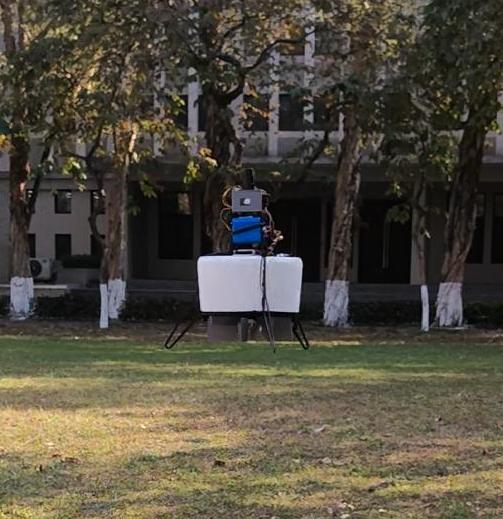
\includegraphics[scale=0.85]{Fig/DFUAV.jpg}
		\label{试验样机}}
        \subfloat[结构组成示意]{
		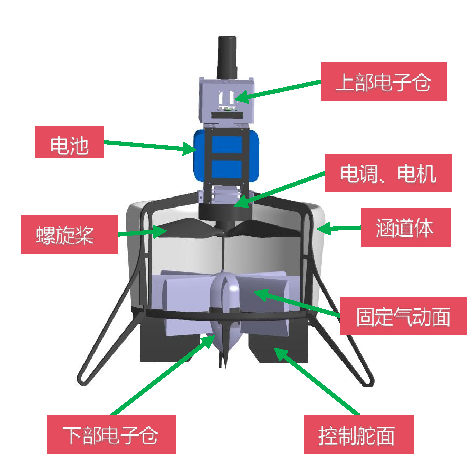
\includegraphics[scale=1]{Fig/涵道结构.pdf}
		\label{主要结构组成}}
        \caption{试验样机及结构组成}\label{DFUAV}
\end{figure}

\subsection{机载航电系统}

图\ref{主要结构组成}中的上部电子仓和下部电子仓共同构成了DFUAV的机载航电系统,掌控着飞行的各个环节,系统内部主要包括微控制器、各种传感器、通信链路等部分。下面对这些部分进行简要介绍:

(1)微控制器(MCU)

    作为DFUAV飞行控制系统的核心处理器,MCU承担着多传感器数据融合与实时决策的关键任务。本系统选用意法半导体公司生产的基于ARM架构的STM32F767系列MCU,其工作频率高达216MHz,通信接口丰富(包括UART/USART、SPI、I2C、CAN等)以及2MB的闪存和512KB的静态随机存储器。其高性能低功耗的特点十分适用于DFUAV的控制。

(2)惯性测量单元(IMU)

    IMU用于测量无人机的加速度和角速度,其输出的数据被用于实时解算无人机的姿态。本系统选用了InvenSense公司的ICM-20602六轴IMU,内部集成了三轴陀螺仪和三轴加速度计。ICM-20602具有高量程($\pm16g$)、大缓冲区(1KB的FIFO)和高精度(误差$\pm1\%$)等特点,并且可以以10MHz的SPI接口或者400kHz的I2C接口输出数据。

(3)磁力计

    磁力计固连在机体上用于测量当前位置的地磁感应强度,其输出的数据结合IMU数据被用于实时解算无人机的航向。本系统选用意法半导体公司的LSM303D系列磁力计,由于测量的数据易受到外界磁场干扰,尤其是电池放电过程中产生的磁场,所以磁力计被安装在远离电池的下部电子仓内。

(4)卫星定位模块

    卫星定位模块用于接收多颗卫星信号来获取无人机的位置和速度等信息。本系统选用了瑞士u-blox公司的ZED-F9P-04B的高精度GPS卫星定位模块,该模块收敛时间快并且方便集成实时动态载波相位差分技术(RTK)实现厘米级的定位精度。
    
(5)气压计

    气压计用于测量当前位置的大气压强并进一步解算出海拔高度。本系统选用的英飞凌公司的DPS368压力传感器,该产品自带防风外壳,基于电容式传感原理在温度变化时依然能保持高精度($\pm0.02m$),可以在恶劣环境中使用。

(6)无线数据传输模块

    无线数据传输模块用于地面站与飞机之间的无线通信,包括由地面站发送给飞机的控制指令和飞机发送到地面站的状态信息等,本方案选用Microhard的hp840无线调制解调器,支持840-845MHz的跳频或定频工作以及理想情况下160公里的传输距离。

在飞行控制周期内,MCU首先首先完成多个传感器设备的协同启动与自检流程,然后通过外设接口读取IMU、磁力计、GPS、气压计等传感器的数据。接下来通过滤波方法对数据进行平滑去噪等处理,并且通过导航算法融合数据解算出无人机的位置、速度、姿态和角速度等状态信息。借助多频段无线数传模块构建的低延迟通信链路,无人机不仅以50Hz刷新率向地面站传输飞行状态遥测数据包,同时实时接收包含航点指令、模式切换、紧急制动等要素的上行控制帧。控制指令与实时飞行状态参数共同输入至飞行控制决策层,经过飞行控制算法处理后,计算出给到执行机构(电机和舵机)的指令,从而实现对飞行器六自由度运动的闭环控制。


\section{坐标系和姿态表示方法}

考虑到无人机的位置变化与姿态变化,基于地面坐标系($\boldsymbol{O}_e-\boldsymbol{X}_e\boldsymbol{Y}_e\boldsymbol{Z}_e $)和机体坐标系(${\boldsymbol{O}_b}-{\boldsymbol{X}_b}{\boldsymbol{Y}_b}{\boldsymbol{Z}_b}$)的多坐标系表示法被广泛应用于无人机的运动分析与控制系统设计中。

% \begin{enumerate}[topsep = 0 pt, itemsep= 0 pt, parsep=0pt, partopsep=0pt, leftmargin=44pt, itemindent=0pt, labelsep=6pt, label=(\arabic*)]
% \item 地面坐标系
(1)地面坐标系

地面坐标系的原点$\boldsymbol{O}_e$可以是地平面上的任意一点,一般定义为无人机的起飞点。三轴方向分别为$\boldsymbol{O}_e-\boldsymbol{X}_e$轴在地平面内指向地理正北方向(N),$\boldsymbol{O}_e-\boldsymbol{Y}_e$轴在地平面内指向地理正东方向(E),$\boldsymbol{O}_e-\boldsymbol{Z}_e$轴按照右手定则,垂直于地面指向地心,方向向下(D)。因此地面坐标系也被称为北东地(NED)坐标系,该坐标系与地球固连。

% \item 机体坐标系
(2)机体坐标系

机体坐标系与无人机的机体固连,其原点$\boldsymbol{O}_b$定义为无人机的重心位置。三轴方向分别为$\boldsymbol{O}_b-\boldsymbol{X}_b$轴在无人机对称平面内指向人为定义的机头方向,$\boldsymbol{O}_b-\boldsymbol{Z}_b$轴在无人机对称平面内垂直于$\boldsymbol{O}_b-\boldsymbol{X}_b$轴向下为正,$\boldsymbol{O}_b-\boldsymbol{Y}_b$轴按照右手定则与$\boldsymbol{X}_b-\boldsymbol{O}_b-\boldsymbol{Z}_b$平面垂直,沿着机身的右侧方向向右为正。
% \end{enumerate}

地面坐标系和机体坐标系定义如图\ref{坐标系}所示。同一个物理量在不同的坐标系中有不同的大小和方向,为便于区分,在全文中统一使用上标$(.)^{e}$与$(.)^{b}$表示同一个物理量分别在地面坐标系和机体坐标系下的表示。

在地面坐标系下采用惯性导航系统、GPS导航等方式,无人机的位置和速度等运动状态可以方便直观地映射到地理空间中。这种方式使得无人机的飞行轨迹与实际地理位置紧密相关,以便进行飞行路线规划和轨迹优化。无人机的重心相对于地面坐标系的位置矢量在地面坐标系下表示为$\boldsymbol{P}^{e}=[{x}^{e} \quad {y}^{e} \quad {z}^{e}]^{T}$,机体重心沿着地面坐标系的速度矢量在地面坐标系下表示为$\boldsymbol{V}^{e}=[{v}^{e}_{x} \quad {v}^{e}_{y} \quad {v}^{e}_{z}]^{T}$,机体重心相对于地面坐标系的速度矢量在机体坐标系下表示为$\boldsymbol{V}^{b}=[{u} \quad {v} \quad {w}]^{T}$。

地面坐标系与机体坐标系的旋转变化关系体现了无人机的姿态变化,无人机常用的姿态描述方法有欧拉角、旋转矩阵和四元数等方式。其中欧拉角表示方法因物理意义明确,表示直观,所以被广泛采用。但因其奇异性问题\cite{全权2018多旋翼飞行器设计与控制},欧拉角表示法在一些特殊场景的使用下受到制约(如滚转角或者俯仰角为$\pm90^{\circ}$的情况)。考虑到本研究在姿态控制中,由于输入姿态指令和输出舵面角度的约束,不会出现上述奇异情况,所以本文采用欧拉角来描述无人机的姿态。根据欧拉定理,地面坐标系按照某个固定点经过三次基本旋转可以得到机体坐标系。由于旋转运动与坐标系原点的位置无关,所以为便于理解,将地面坐标系的原点与机体坐标系原点重合(即$\boldsymbol{O}_e=\boldsymbol{O}_b$),如图\ref{欧拉角}所示。在三次基本旋转中,旋转轴是待转动坐标系的某一轴,旋转的角度即为欧拉角。由于姿态旋转矩阵可以表示为三次基本旋转的乘积,所以与旋转顺序密切相关。由于本研究不会出现奇异问题,所以本文采用常用的‘Z-Y-X’的旋转顺序的欧拉角表示法。

\begin{figure}[htbp]
	\centering
	\begin{minipage}[c]{0.5\textwidth}
		\centering
		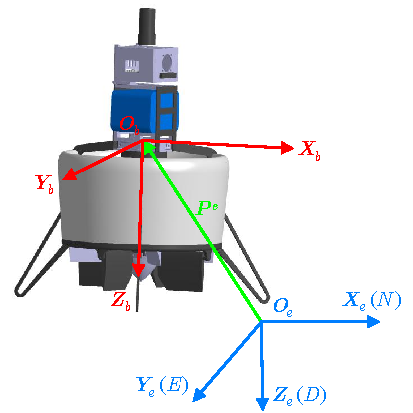
\includegraphics[scale=1]{Fig/坐标系.pdf}
		\caption{\label{坐标系}地面坐标系与机体坐标系定义}
	\end{minipage}%
    \begin{minipage}[c]{0.5\textwidth}
		\centering
		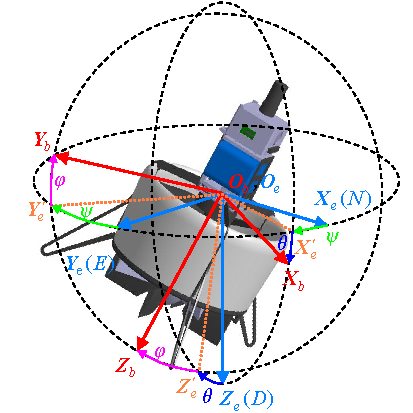
\includegraphics[scale=1]{Fig/欧拉角.pdf}
		\caption{\label{欧拉角}‘Z-Y-X’欧拉角的定义}
	\end{minipage}%
\end{figure}

在图\ref{欧拉角}中,地面坐标系$\boldsymbol{O}_e-\boldsymbol{X}_e\boldsymbol{Y}_e\boldsymbol{Z}_e$首先围绕$\boldsymbol{Z}_e$轴旋转偏航角$\psi$,向右偏航为正方向。此时$\boldsymbol{X}_e$轴旋转至$\boldsymbol{X}_e^{'}$轴,$\boldsymbol{Y}_e$轴旋转至$\boldsymbol{Y}_e^{'}$轴,$\boldsymbol{Z}_e$轴保持不变;
然后临时坐标系$\boldsymbol{O}_e-\boldsymbol{X}_e^{'}\boldsymbol{Y}_e^{'}\boldsymbol{Z}_e$围绕$\boldsymbol{Y}_e^{'}$轴旋转俯仰角$\theta$,上仰为正方向。此时$\boldsymbol{X}_e^{'}$轴旋转至$\boldsymbol{X}_b$轴,与机体系保持一致,$\boldsymbol{Z}_e$轴旋转至$\boldsymbol{Z}_e^{'}$轴,$\boldsymbol{Y}_e^{'}$轴保持不变;
最后临时坐标系$\boldsymbol{O}_e-\boldsymbol{X}_b\boldsymbol{Y}_e^{'}\boldsymbol{Z}_e^{'}$围绕$\boldsymbol{X}_b$轴旋转滚转角$\varphi$,向右滚转为正方向。此时$\boldsymbol{Y}_e^{'}$轴旋转至$\boldsymbol{Y}_b$轴,$\boldsymbol{Z}_e^{'}$轴旋转至$\boldsymbol{Z}_b$轴,均与机体系保持一致。

三次基本旋转的角度分别为$\psi$、$\theta$、$\varphi$,定义其对应的旋转矩阵分别为$\boldsymbol{R}_\psi,\boldsymbol{R}_\theta,\boldsymbol{R}_\varphi\in{SO(3)}$,其中$SO(3)=\{\boldsymbol{R}\in\mathbb{R}^{3\times3}|\boldsymbol{R}\boldsymbol{R}^T=I,|\boldsymbol{R}|=1\}$。
\begin{equation}
    \begin{aligned} %表示公式编号上下居中
\boldsymbol{R}_\psi=\begin{bmatrix}\cos\psi & \sin\psi & 0 \\-\sin\psi & \cos\psi & 0 \\0 & 0 & 1\end{bmatrix},\boldsymbol{R}_\theta=\begin{bmatrix}\cos\theta & 0 & -\sin\theta \\0 & 1 & 0 \\\sin\theta & 0 & \cos\theta\end{bmatrix},\boldsymbol{R}_\varphi=\begin{bmatrix}1 & 0 & 0\\0 & \cos\varphi & \sin\varphi \\0 & -\sin\varphi & \cos\varphi\end{bmatrix}\label{eq_1}
    \end{aligned}
\end{equation}

为表述方便,定义如下单位向量:
\begin{equation}
    \begin{aligned}
\boldsymbol{e}_1=\begin{bmatrix}1 \\0 \\0\end{bmatrix},
\quad\boldsymbol{e}_2=\begin{bmatrix}0 \\1 \\0\end{bmatrix},
\quad\boldsymbol{e}_3=\begin{bmatrix}0 \\0 \\1\end{bmatrix}\label{eq_2}
    \end{aligned}
\end{equation}

机体姿态的欧拉角表示为$\boldsymbol{\eta}=[\varphi \quad \theta \quad \psi]^T$,对应的姿态变化率为$\boldsymbol{\dot{\eta}}=[\dot{\varphi} \quad \dot{\theta} \quad \dot{\psi}]^T$。定义沿机体轴的旋转角速度为$\boldsymbol{\omega}^b=[p \quad q \quad r]^T$,那么旋转角速度与机体姿态变化率的关系如下\cite{ducard2009fault}:
\begin{equation}
    \boldsymbol\omega^{b}=\dot{\psi}\boldsymbol{R}_{\varphi} \boldsymbol{R}_{\theta} \boldsymbol{e}_{3}+\dot{\theta}\boldsymbol{R}_{\varphi}\boldsymbol{e}_{2}+\dot{\varphi}\boldsymbol{e}_{1}\label{eq_3}
\end{equation}
结合式\eqref{eq_1}、式\eqref{eq_2}和式\eqref{eq_3},得到:
\begin{equation}
    \begin{gathered}
    \boldsymbol\omega^{b}=
    \begin{bmatrix}
    1 & 0 & -\sin\theta \\
    0 & \cos\varphi & \sin\varphi\cos\theta \\
    0 & -\sin\varphi & \cos\varphi\cos\theta
    \end{bmatrix}
    \boldsymbol{\dot{\eta}}
    \\
    \Leftrightarrow\dot{\boldsymbol{\eta}}=\boldsymbol{Q}\boldsymbol{\omega}^b,\quad\boldsymbol{Q}\triangleq
    \begin{bmatrix}
        1 & \sin\varphi\tan\theta & \cos\varphi\tan\theta \\
        0 & \cos\varphi & -\sin\varphi \\
        0 & \dfrac{\sin\varphi}{\cos\theta} & \dfrac{\cos\varphi}{\cos\theta}
        \end{bmatrix}
    \label{eq_4}
    \end{gathered}
\end{equation}

进一步地,在欧拉角‘Z-Y-X’的旋转顺序下,由机体坐标系到地面坐标系的旋转矩阵$\boldsymbol{R}^e_b$可以表示为:
\begin{equation}
    \begin{aligned}
    \boldsymbol{R}_{b}^{e} & =(\boldsymbol{R}_{e}^{b})^T =(\boldsymbol{R}_\varphi\boldsymbol{R}_\theta\boldsymbol{R}_\psi)^T \\
     & =
    \begin{bmatrix}
    \cos{\theta}\cos{\psi} & \sin{\varphi}\sin{\theta}\cos{\psi}-\cos{\varphi}\sin{\psi} & \cos{\varphi}\sin{\theta}\cos{\psi} + \sin{\varphi}\sin{\psi}
    \\ 
    \cos{\theta}\sin{\psi} & \sin{\varphi}\sin{\theta}\sin{\psi} + \cos{\varphi}\cos{\psi} & \cos{\varphi}\sin{\theta}\sin{\psi} - \sin{\varphi}\cos{\psi}
    \\
    -\sin{\theta} & \sin{\varphi}\cos{\theta} & \cos{\varphi}\cos{\theta}
    \end{bmatrix}
    \label{eq_5}
    \end{aligned}
\end{equation}

\section{飞行控制刚体模型}

DFUAV的建模过程需要在准确性与实用性之间找到合适的平衡,确保不会过于复杂而增加控制算法设计的难度和计算资源的开销,同时也不至于过于简单而与实际情况相差甚远。因此,在建模过程中假设DFUAV是刚体,并且假设DFUAV在飞行过程中其质量和转动惯量(机体坐标系下)保持不变。基于这种假设,DFUAV的刚体运动学和动力学模型可以通过牛顿-欧拉方法推导得到。

\subsection{刚体运动学模型}

运动学模型用于描述无人机在三维空间中的位置和姿态随时间变化的关系,不涉及力与力矩的分析。六自由度DFUAV的刚体运动学模型包括三自由度的位置运动学模型和三自由度的姿态运动学模型。在地面坐标系下,位置运动学模型可以表示为:$\boldsymbol{\dot{P}}^{e} = \boldsymbol{V}^{e}$。三自由度的姿态运动学模型分为欧拉角模型、旋转矩阵模型和四元数模型三种。在机体系下,根据式\eqref{eq_4},可以得到使用欧拉角模型表示三自由度的姿态运动学为$\dot{\boldsymbol{\eta}}=\boldsymbol{Q}\boldsymbol{\omega}^b$。

因此,六自由度的DFUAV刚体运动学模型可以表示为:
\begin{equation}
    \begin{aligned}
    \boldsymbol{\dot{P}}^{e} &= \boldsymbol{V}^{e} \\
    \dot{\boldsymbol{\eta}}&=\boldsymbol{Q}\boldsymbol{\omega}^b
    \end{aligned}
    \label{eq_6}
\end{equation}

\subsection{刚体动力学模型}

DFUAV的刚体动力学模型包括位置动力学模型和姿态动力学模型,动力学模型是描述无人机在三维空间中运动行为的数学模型,该模型主要基于牛顿第二定律和角动量定理推导,用于分析无人机在受力、力矩、环境扰动等因素共同作用下的运动行为。但是该定律仅在惯性系下成立,考虑到DFUAV的在运动时,地球自转对其的影响相对不显著,并且从局部来看,地面近似平坦,因此将地面坐标系假设为惯性系是合理的。

假设DFUAV受到的力包括重力和除重力之外的合外力作用$\boldsymbol{F}^b$,为下文受力分析方便,此处$\boldsymbol{F}^b\in\mathbb{R}^{3\times1}$表示在机体系下受到的除重力之外的合外力。那么根据牛顿第二定律可以得到:
\begin{equation}
    \begin{gathered}
    \boldsymbol{R}_b^e\boldsymbol{F}^b + mg\boldsymbol{e}_3 = m\dfrac{d({\boldsymbol{V}}^e)}{dt}
    \\
    \Leftrightarrow\dot{\boldsymbol{V}}^e=\dfrac{1}{m}\boldsymbol{R}_b^e\boldsymbol{F}^b + g\boldsymbol{e}_3 
    \label{eq_7}
    \end{gathered}
\end{equation}
其中$m$表示DFUAV的总质量,$g$表示当地的重力加速度。

姿态动力学模型由角动量定理描述:
\begin{equation}
    \begin{gathered}
    \boldsymbol{M}^{b}=\dfrac{d\boldsymbol{L}^{b}}{dt} - {\boldsymbol{L}^{b}}\times{\boldsymbol\omega^{b}},\quad \boldsymbol{L}^{b}=\boldsymbol{J}^{b}\boldsymbol\omega^{b}
    \\
    \Leftrightarrow\boldsymbol{\dot{\omega}}^b=(\boldsymbol{J}^b)^{-1}(\boldsymbol{M}^b+\boldsymbol{J}^b\boldsymbol{\omega}^b\times\boldsymbol{\omega}^b)
    \label{eq_8}
    \end{gathered}
\end{equation}
其中$\boldsymbol{M}^{b}\in\mathbb{R}^{3\times1}$表示DFUAV在机体系下受到的合外力矩,$\boldsymbol{L}^{b}\in\mathbb{R}^{3\times1}$表示DFUAV在机体系下总的角动量,‘$\times$’表示向量叉乘运算。$\boldsymbol{J}^{b}\in\mathbb{R}^{3\times3}$表示DFUAV在机体系中的转动惯量矩阵,其在机体系下是一个常量。根据图\Ref{DFUAV},可以看出本文研究的DFUAV呈现对称的几何结构,故本文建模过程中认为$\boldsymbol{J}^{b}$近似为一个对角矩阵,即
\begin{equation}
    \boldsymbol{J}^b=\begin{bmatrix}
        J_{x} & 0 & 0 \\
        0 & J_{y} & 0 \\
        0 & 0 & J_{z}
        \end{bmatrix}
    \label{eq_9}
\end{equation}

类似地,在机体系下可以更加直观地表示姿态动力学模型中相关变量,并且便于下文对力矩的分析,其中${\boldsymbol{L}^{b}}\times{\boldsymbol\omega^{b}}$部分分量表示由惯性系旋转到机体系产生的影响。

综合上述分析,可以得到DFUAV的飞行控制刚体模型:
\begin{equation}
    \left\{
    \begin{aligned}
        \boldsymbol{\dot{P}}^{e} &= \boldsymbol{V}^{e} \\
        \dot{\boldsymbol{V}}^e&=\dfrac{1}{m}\boldsymbol{R}_b^e\boldsymbol{F}^b + g\boldsymbol{e}_3 \\
        \dot{\boldsymbol{\eta}}&=\boldsymbol{Q}\boldsymbol{\omega}^b \\
        \boldsymbol{\dot{\omega}}^b&=(\boldsymbol{J}^b)^{-1}(\boldsymbol{M}^b+\boldsymbol{J}^b\boldsymbol{\omega}^b\times\boldsymbol{\omega}^b)
    \end{aligned}
    \right.
    \label{eq_10}
\end{equation}

\section{力与力矩分析}

对作用于DFUAV上的力与力矩进行分析是为了对下文控制算法的设计提供物理依据,明确力与力矩的来源与作用方式对于分析DFUAV的运动特性至关重要。根据式\eqref{eq_10},DFUAV受到的除重力作用外的合外力在机体系下表示为$\boldsymbol{F}^b$,受到的合外力矩在机体系下表示为$\boldsymbol{M}^b$。进一步地,$\boldsymbol{F}^b$和$\boldsymbol{M}^b$可以被分解为:
\begin{equation}
    \left\{
    \begin{aligned}
        \boldsymbol{F}^b&=\boldsymbol{F}_{fan}^b+\boldsymbol{F}_{aero}^b+\boldsymbol{F}_{duct}^b+\boldsymbol{F}_{vane}^b \\
        \boldsymbol{M}^b&=\boldsymbol{M}_{fan}^b+\boldsymbol{M}_{aero}^b+\boldsymbol{M}_{duct}^b+\boldsymbol{M}_{vane}^b+\boldsymbol{M}_{gyro}^b+\boldsymbol{M}_{flap}^b
    \end{aligned}
\right.
\label{eq_11}
\end{equation}
其中$\boldsymbol{F}_{fan}^b$和$\boldsymbol{M}_{fan}^b$表示由于涵道风扇旋转而产生的总的拉力和扭矩,$\boldsymbol{F}_{aero}^b$和$\boldsymbol{M}_{aero}^b$表示由于机身空气阻力产生的气动力和力矩,$\boldsymbol{F}_{duct}^b$和$\boldsymbol{M}_{duct}^b$表示作用于涵道环翼上的气动力与力矩,$\boldsymbol{F}_{vane}^b$和$\boldsymbol{M}_{vane}^b$表示由于涵道底部的控制舵面运动与风扇滑流相互作用而产生的力和力矩,$\boldsymbol{M}_{gyro}^b$表示由于涵道风扇的旋转而产生的陀螺力矩,$\boldsymbol{M}_{flap}^b$表示位于涵道底部的固定气动面于风扇滑流相互作用而产生的扭矩。下面将对各力与力矩的作用机理进行逐一分析。

\subsection{涵道风扇动力学}

涵道风扇是安装在圆形涵道内的螺旋桨,旋翼模型的研究主要基于基本动量理论和叶素理论。由于涵道入口边缘的吸力效应和出口处较高的静压的共同作用,相比于开放式的螺旋桨,在相同的功率下,涵道风扇具有更出色的静态性能。

可以使用动量理论进行悬停情况下的分析,在相同的功率条件下,推力增益可以描述为扩张比的函数:
\begin{equation}
    \dfrac{\boldsymbol{F}_{fan}^b}{\boldsymbol{F}_{prop}}={\sqrt[3]{2\Lambda}}
    \label{eq_12}
\end{equation}
其中$\boldsymbol{F}_{fan}^b$是由于涵道风扇旋转产生的总拉力,设其标量表示为$T_{fan}$。$T_{fan}$可以分为两部分:涵道风扇旋转产生的拉力$T_{p}$和侧风与涵道风扇抽吸作用产生的侧向拉力$T_{l}$。$\boldsymbol{F}_{prop}$表示传统开放式螺旋桨产生的拉力,$\Lambda$是扩张比。由式\eqref{eq_12}可以看出,扩张比大于0.5时,涵道风扇的推力增益大于1,即涵道风扇比开放式旋翼的推力效率更高。更详尽的分析可以在\parencite{pereiraHoverWindtunnelTesting2008}中找到。

% 据此定义涵道拉力分配系数:
% \begin{equation}
%     \lambda=\dfrac{T_{p}}{T_{fan}}=\dfrac{T_{p}}{T_{p}+T_{l}}
%     \label{eq_13}
% \end{equation}

% 由于涵道的遮挡作用,涵道出口的气流基本保持轴向流动,沿着轴线方向喷射出去,如图所示。假设空气密度为$\rho$,气流在未受到涵道风扇影响前的速度和压强分别为$V_0$和$p_0$,气流在逼近涵道风扇上表面时的速度增加为$V_1$同时压强减小为$p_1$。忽略风扇的厚度,气流通过风扇到下表面即将进入滑流区时,由于气流速度连续不可突变,所以认为气流速度保持$V_2=V_1$,但压强增加为$p_1+\Delta p$。气流进入滑流区后,速度进一步增大为$V_e$,压强恢复到来流状态$p_0$。在涵道风扇的上下表面分别应用伯努利方程:

% \noindent 上表面
% \begin{equation}
%         p_0+\frac{1}{2}\rho V_0^2=p_1+\frac{1}{2}\rho V_1^2
%     \label{eq_14}
% \end{equation}
% 下表面
% \begin{equation}
%     p_1+\Delta p+\frac{1}{2}\rho V_2^2=p_0+\frac{1}{2}\rho V_e^2
%     \label{eq_15}
% \end{equation}
% 所以涵道风扇上下表面的压强差为:
% \begin{equation}
%     \Delta p=\frac{1}{2}\rho(V_e^2-V_0^2)
%     \label{eq_16}
% \end{equation}

由于涵道的遮挡作用,涵道出口的气流基本保持轴向流动,沿着轴线方向喷射出去,如图\ref{轴流管道模型}所示。假设气流在未受到涵道风扇影响前的速度为$V_0$,在逼近涵道风扇上表面时的速度增加为$V_1$。忽略风扇的厚度,气流通过风扇到下表面即将进入滑流区时,由于气流速度连续不可突变,所以认为气流速度保持$V_2=V_1$。气流进入滑流区后,速度进一步增大为$V_e$并从涵道下方出口排出。

\begin{figure}[htbp]
	\centering
	\begin{minipage}[c]{1\textwidth}
		\centering
		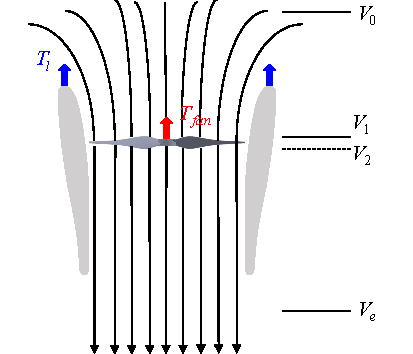
\includegraphics[scale=1]{Fig/轴流管道模型.pdf}
		\caption{\label{轴流管道模型}轴流状态的空气动力学}
	\end{minipage}%
\end{figure}

假设风扇旋转时的桨盘面积为$S$,涵道扩压比为$\sigma_d$,$\sigma_d$表示涵道下方出口横截面面积与桨盘面积$S$之比。那么根据质量守恒有:
\begin{equation}
    \sigma_dSV_e=SV_2=SV_1
    \label{eq_17}
\end{equation}

设空气密度为$\rho$,单位时间内通过涵道风扇的气流总质量为$\dot{m}_{air}$。一方面,根据动量定理可知,涵道风扇对气流施加的总作用力等于单位时间内气流通过风扇的动量变化率:
\begin{equation}
    T_{fan}=\dot{m}_{air}(V_e-V_0)=\rho S V_1(V_e-V_0)
    \label{eq_18}
\end{equation}
另一方面,气体动能的变化量等同于涵道风扇输送给气体的功率:
\begin{equation}
    \frac{1}{2}\dot{m}_{air}V_e^2-\frac{1}{2}\dot{m}_{air}V_0^2=T_{fan}V_1
    \label{eq_19}
\end{equation}
结合\eqref{eq_17}、\eqref{eq_18}和\eqref{eq_19},可以得到涵道出口风速$V_e$\cite{pereiraHoverWindtunnelTesting2008}:
\begin{equation}
    V_e=\frac{V_0}{2}+\sqrt{\left(\frac{V_0}{2}\right)^2+\frac{T_{fan}}{\sigma_d\rho S}}    \label{eq_20}
\end{equation}
定义涵道风扇的诱导速度为$V^{\prime}=V_1-V_0$,那么结合\eqref{eq_17}和\eqref{eq_20}可以得到:
\begin{equation}
    \begin{aligned}
    V^{\prime}&=\sigma_dV_e-V_0 \\
    &=\left(\frac{\sigma_d}{2}-1\right)V_0+\sqrt{\left(\frac{V_0\sigma_d}{2}\right)^2+\frac{T_{fan}\sigma_d}{\rho S}}
    \label{induced velocity}
    \end{aligned}
\end{equation}
涵道出口处的气流速度$V_e$和涵道风扇的诱导速度$V^{\prime}$将在后续的空气动力学分析中发挥重要作用,包括涵道翼型上产生的附加阻力的计算、控制舵面上的力与力矩的计算以及固定气动面扭矩的计算等。

关于涵道风扇产生的拉力$T_{p}$、侧向拉力$T_{l}$和扭矩$\boldsymbol{M}_{fan}^b$的计算,由下式给出\cite{luoNumericalAnalysisWind2024a}:
\begin{equation}
    \begin{aligned}
        T_{p}&=\rho S \Omega^2R^2 C_{p}\\
        T_{l}&=\rho S \Omega^2R^2 C_{l}\\
        \boldsymbol{M}_{fan}^b&=\rho S \Omega^2 R^3C_{q}
    \end{aligned}
    \label{eq_21}
\end{equation}
其中$\Omega$是涵道风扇的旋转角速度,$R$是涵道风扇的旋转半径,$C_{p}$、$C_{l}$和$C_{q}$分别是涵道风扇的拉力系数、侧向推力系数和扭矩系数。这三个系数与环境风速、飞机姿态等因素有关,难以用简单的解析式来表示。大部分文献都采用数值分析方法来测定\cite{iiiNondimensionalModelingDuctedFan2012,choiStaticAnalysisSmall2012,luoNumericalAnalysisWind2024a}。

由于$\rho$、$S$、$R$均为常数,涵道风扇产生的总的拉力$\boldsymbol{F}_{fan}^b$和扭矩$\boldsymbol{M}_{fan}^b$仅在机体系下的${\boldsymbol{O}_b}-{\boldsymbol{Z}_b}$轴产生效果,所以可以近似简化为以下形式\cite{choiStaticAnalysisSmall2012,manzoorCompositeObserverbasedRobust2023}:
\begin{align}
            \boldsymbol{F}_{fan}^b=\begin{bmatrix}0 \\ 0 \\
                -k_{fan}\Omega^2
            \end{bmatrix},\quad    
            \boldsymbol{M}_{fan}^b=\begin{bmatrix}0 \\ 0 \\
            -k_{q}\Omega^2
            \end{bmatrix}    \label{eq_22}
\end{align}
其中$k_{fan}$和$k_{q}$均为常系数,可采用数值分析方法近似测定。
\subsection{机身动力学}

涵道机身的气动阻力和力矩源于机身与气流错综复杂的相互作用。当无人机在空中飞行时,周围的气流会以一定的速度与涵道机身表面接触。这种相互碰撞、摩擦,形成了阻碍飞机前进的气动阻力。同时,由于气流在机身不同部位的速度和压强分布不均匀,会对机身产生一个使它绕某一轴转动的趋势,这便是气动力矩。根据空气动力学原理,气动阻力与飞机与气流相对速度的平方大致成正比关系。而且速度的变化还会影响气流在机身周围的流动形态,使得气动力矩也发生相应变化。另外,沿机体轴方向的横截面积同样是影响气动阻力和力矩的重要因素。较大的横截面积意味着气流与机身的接触面积更大,气流在流经机身时受到的阻碍也会增加。由于DFUAV的外部由涵道体包裹,因此横截面积较大,更会加剧这一过程。

定义空速向量$\boldsymbol{V}_a^b= [ u_r \quad v_r \quad w_r ]^T$为机体相对于气流的速度在机体系的投影,标量表示为$V_a$,空速与环境风速有关。当环境风速$\boldsymbol{W}^e$为零时,$\boldsymbol{V}_a^b=\boldsymbol{V}^b$。在机身产生的力与力矩可表示为\cite{johnsonModelingControlFlight2006b,choiStaticAnalysisSmall2012}:
\begin{gather}
    \boldsymbol{F}_{aero}^b=-\frac{1}{2}\rho
    \begin{bmatrix}
    C_{D,x}S_xu_r|u_r| \\
    C_{D,y}S_yv_r|v_r| \\
    C_{D,z}S_zw_r|w_r|
    \end{bmatrix}\label{eq_22.5}\\
    \boldsymbol{M}_{aero}^b=\frac{1}{2}\rho
    \begin{bmatrix}
    C_{D,y}S_yv_r|v_r| \\
    -C_{D,x}S_xu_r|u_r| \\
    0
    \end{bmatrix}l_{a}
    \label{eq_23}
\end{gather}
其中$C_{D,x}$、$C_{D,y}$和$C_{D,z}$分别是机身沿机体系三个轴方向的气动阻力系数,$S_x$、$S_y$和$S_z$分别是机身沿机体系三个轴方向的横截面积,$l_{a}$表示DFUAV的机身空气动力中心和其重心之间的距离。

由$\boldsymbol{M}_{aero}^b$的表达式可以看出,机身气动力矩不会影响机体系下的${\boldsymbol{O}_b}-{\boldsymbol{Z}_b}$轴,暗含DFUAV的空气动力中心和其重心之间的距离在${\boldsymbol{O}_b}-{\boldsymbol{X}_b}$轴和${\boldsymbol{O}_b}-{\boldsymbol{Y}_b}$轴上的分量为零,这是由于DFUAV的几何对称特性所导致的。

\subsection{涵道动力学}

类似直升机旋翼的经典建模方法,本小节基于不可压缩的定常流动假设建立升力$L$-阻力$D$模型来估算空速施加在涵道环翼上的气动力与力矩\cite{johnsonModelingControlFlight2006b},如图\ref{非轴流状态}所示。

\begin{figure}[htbp]
	\centering
	\begin{minipage}[c]{1\textwidth}
		\centering
		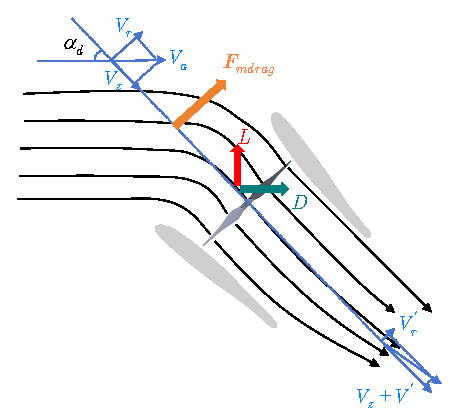
\includegraphics[scale=1]{Fig/非轴流状态.pdf}
		\caption{\label{非轴流状态}非轴流状态(前飞时)的空气动力学}
	\end{minipage}%
\end{figure}

假设$\gamma$代表在机体系${\boldsymbol{O}_b}-{\boldsymbol{X}_b}{\boldsymbol{Y}_b}$平面内的角度度量,$\boldsymbol{i}$和$\boldsymbol{j}$分别表示沿着机体系${\boldsymbol{O}_b}-{\boldsymbol{X}_b}$轴和${\boldsymbol{O}_b}-{\boldsymbol{Y}_b}轴$的单位向量。那么在${\boldsymbol{O}_b}-{\boldsymbol{X}_b}{\boldsymbol{Y}_b}$平面内的单位向量和速度向量可以表示为:
\begin{align}
    \boldsymbol{e}_{r}&=\cos\gamma\boldsymbol{i}+\sin\gamma\boldsymbol{j} \label{eq_24}\\
    \boldsymbol{V}_{xy}&=-u_r\boldsymbol{i}-v_r\boldsymbol{j} \label{eq_25}
\end{align}
由于式\eqref{eq_25}中的速度表示机体相对于气流的速度,为表示气流相对于机体的速度需要加负号。为方便表示,假设在涵道周围沿${\boldsymbol{O}_b}-{\boldsymbol{Z}_b}$轴方向的速度分量是恒定的。那么径向速度${V}_{r}(\gamma)$作为$\gamma$的函数可以写为:
\begin{equation}
    V_r(\gamma)=\boldsymbol{V}_{xy}\cdot{\boldsymbol{e}}_r=-u_r\cos\gamma-v_r\sin\gamma    \label{eq_26}
\end{equation}
气流速度在${\boldsymbol{O}_b}-{\boldsymbol{Z}_b}$轴方向相对于机体的速度分量$V_z(\gamma)$可以表示为:
\begin{equation}
    V_z(\gamma)=-w_r   \label{eq_27}
\end{equation}
其中诱导速度$V^{\prime}$于式\eqref{induced velocity}中定义。

现在,涵道周围的动态压力$q_d(\gamma)$和迎角$\alpha_d(\gamma)$可以如下计算:
\begin{equation}
    \begin{aligned}
        q_d(\gamma)&=\frac{1}{2}\rho\left(V_r^2+V_z^2\right)\\
        \alpha_d(\gamma)&=\tan^{-1}\left(\frac{V_r}{V_z}\right)
    \label{eq_28}
    \end{aligned}
\end{equation}
根据式\eqref{eq_28}进一步可以表示出涵道周围单位展长的升力$l(\gamma)$和阻力$d(\gamma)$及其在每个机体轴的分量:
\begin{equation}
        l(\gamma)=C_{l,d}(\alpha_d)c_dq_d, \quad
        d(\gamma)=C_{d,d}(\alpha_d)c_dq_d
    \label{eq_29}
\end{equation}
\begin{equation}
        \begin{aligned}
            \Rightarrow
        l_{x}(\gamma)&=l(\gamma)\cos\alpha_d\cos\gamma,\quad d_x(\gamma)=d(\gamma)\sin\alpha_d\cos\gamma \\
        l_{y}(\gamma)&=l(\gamma)\cos\alpha_d\sin\gamma,\quad d_y(\gamma)=d(\gamma)\sin\alpha_d\sin\gamma \\
        l_{z}(\gamma)&=-l(\gamma)\sin\alpha_d,\quad d_z(\gamma)=d(\gamma)\cos\alpha_d
        \label{eq_30}
    \end{aligned}
\end{equation}
式\eqref{eq_29}中$C_{l,d}$、$C_{d,d}$分别是涵道翼型的升力曲线和阻力曲线,均与迎角$\alpha_d(\gamma)$有关。$c_d$是涵道翼型的弦长。将式\eqref{eq_30}中的各轴向分量沿该轴方向积分便可得到每个轴的气动升力和阻力,如$x$轴方向:
\begin{equation}
    L_x=R\int_0^{2\pi}l_x(\gamma)d\gamma, \quad
    D_x=R\int_0^{2\pi}d_x(\gamma)d\gamma
    \label{eq_31}
\end{equation}

除气动升力和阻力外,DFUAV前飞时(非轴流状态)在涵道上还会产生附加的阻力(即动量阻力$\boldsymbol{F}_{mdrag}$\cite{choiStaticAnalysisSmall2012})。如图\ref{非轴流状态}所示,由于涵道体的遮挡,气流的径向速度$V_r$分量在进入涵道体后迅速衰减为$V_r^\prime$,因此导致径向气体动量的变化,从而产生附加的阻力。该阻力可以通过进入涵道的空气质量流量和飞行速度来表示:
\begin{equation}
    \boldsymbol{F}_{mdrag}=-V^\prime\rho{S}
    \begin{bmatrix}u_r \\v_r \\0
    \end{bmatrix}
    \label{eq_32}
\end{equation}

侧风作用于涵道结构形成的的非对称升力分布同样会产生力矩,假定该力矩与侧风引起的动态压力为近似线性关系,那么可量化为:
\begin{equation}
    \boldsymbol{M}_{lip}=C_{duct}\rho{R}
    \begin{bmatrix}v_r|v_r| \\-u_r|u_r| \\0\end{bmatrix}
    \label{eq_33}
\end{equation}
其中,$C_{duct}$是常系数。该系数最初可根据iSTAR\cite{flemingImprovingControlSystem}的实验数据估算,随后需要结合实际情况调整。

综合\eqref{eq_31}、\eqref{eq_32}、\eqref{eq_33},在涵道翼型上产生的力与力矩可以表示为\cite{johnsonModelingControlFlight2006b,choiStaticAnalysisSmall2012}:
\begin{align}
    \boldsymbol{F}_{duct}^b=
    \begin{bmatrix}
    L_x+D_x \\
    L_y+D_y \\
    L_z+D_z
    \end{bmatrix}+\boldsymbol{F} _{mdrag}\label{eq_33.5}\\
    \boldsymbol{M}_{duct}^b=
    \begin{bmatrix}
    L_xl_d \\
    L_yl_d \\
    0
    \end{bmatrix}+\boldsymbol{M}_{lip}
    \label{eq_34}
\end{align}
其中$l_d$表示DFUAV的重心与涵道空气动力中心之间的距离。

\subsection{控制舵面动力学}

涵道底部的控制舵面是DFUAV的主要控制机构,在飞行过程中控制舵面的运动会产生气动力和力矩,这些力矩是造成DFUAV进行滚转、俯仰、偏航姿态变化的主要原因。如图\ref{控制舵面}所示,本文研究的DFUAV配置有四片交叉排列的控制舵面,定义机体系${\boldsymbol{O}_b}-{\boldsymbol{X}_b}$轴正方向下方位置对应的控制舵面为1号舵,从上往下按照顺时针方向依次编号为2、3、4号舵。1、3号舵的同向运动用于产生滚转力矩,2、4号舵的同向运动用于产生俯仰力矩,4个舵的共同差动用于产生偏航力矩。定义控制舵面的偏转角度为$\boldsymbol{\delta}=[\delta_1\quad\delta_2\quad\delta_3\quad\delta_4]^T$,分别对应4个控制舵面。规定向右偏转为正方向,零位点保持与机体系${\boldsymbol{O}_b}-{\boldsymbol{Z}_b}$轴平行。

\begin{figure}[htbp]
	\centering
	\begin{minipage}[c]{0.5\textwidth} % minipage将页面划分为0.5\textwidth
		\centering
		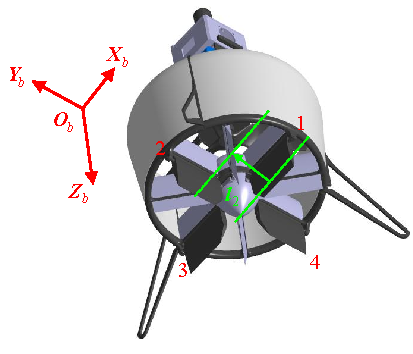
\includegraphics[scale=1]{Fig/控制舵面.pdf}
	\end{minipage}%
	\begin{minipage}[c]{0.5\textwidth}
		\centering
		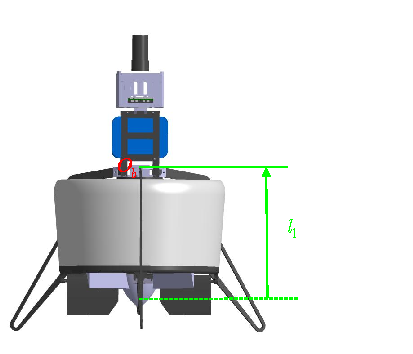
\includegraphics[scale=1]{Fig/力臂.pdf}
	\end{minipage}
    \caption{\label{控制舵面}控制舵面及力臂示意图}
\end{figure}

在涵道风扇滑流中,控制舵面的偏转而产生的升力与机体系${\boldsymbol{O}_b}-{\boldsymbol{Z}_b}$轴垂直,且与转角$\delta_i$的平方成正比\cite{pflimlinModelingAttitudeControl2010a}:
\begin{equation}
    F_i=k_\delta{V_e}^2\delta_i \quad i=1,2,3,4
    \label{eq_35}
\end{equation}
其中$k_\delta$是正的常数,表示控制舵面升力系数。${V_e}$为涵道出口风速,由式\eqref{eq_20}给出。

因此,由控制舵面产生的合力与合力矩可以表示为\cite{pflimlinModelingAttitudeControl2010a,manzoorCompositeObserverbasedRobust2023}:
    \begin{gather}
    \boldsymbol{F}_{vane}^b=\begin{bmatrix}
    F_4-F_2 \\ F_1-F_3 \\ 0 
    \end{bmatrix}     \label{eq_35.5}\\
    \boldsymbol{M}_{vane}^b=\begin{bmatrix}
        -l_1(F_1-F_3) \\ l_1(F_4-F_2) \\ l_2(F_1+F_2+F_3+F_4) 
    \end{bmatrix}
    \label{eq_36}
    \end{gather}
式\eqref{eq_36}中的$l_1$和$l_2$分别为涵道的力臂,如图\ref{控制舵面}所示。事实上,控制舵面的偏转角仅在DFUAV的失速迎角的范围内才有效果\cite{9787121348440000},超出该范围后,姿态将难以控制。因此需要对偏转角度进行限幅处理:
\begin{equation}
    -\delta_m\leq\delta_{i}\leq\delta_m,\quad i=1,2,3,4
    \label{eq_37}
\end{equation}
对于本文研究的DFUAV,限幅值$\delta_m$取$40^\circ$。

\subsection{陀螺力矩与固定气动面反扭矩}

涵道风扇在高速旋转时,DFUAV整体会呈现出类似陀螺的特性。根据角动量守恒定律,当涵道风扇的旋转轴在外力影响下发生偏移时,为了维持整个系统角动量的守恒,涵道风扇会产生一个特殊的反作用力矩。该力矩垂直于旋转轴的偏移方向,试图将旋转轴拉回到原来的方向,从而抵抗外力对旋转状态的干扰。这种作用力矩即为陀螺力矩,其大小与风扇的转动惯量和旋转的角速度有关。转动惯量体现了涵道风扇抵抗转动状态改变的能力,它取决于风扇的质量分布以及形状等因素。角速度反映了风扇旋转的快慢程度。当风扇以较高的角速度旋转时,角动量也较大,为了维持角动量而产生的陀螺力矩也越大。所以有:
\begin{equation}
    \boldsymbol{M}_{gyro}^b=J_{fan}\Omega
    \begin{bmatrix}
    -q \\ p \\ 0
    \end{bmatrix}
    \label{eq_38}
\end{equation}
其中$J_{fan}$为涵道风扇的转动惯量。

固定气动面是指位于涵道内部,涵道风扇下方的固定装置。其特殊的外形结构用于在涵道风扇滑流中产生反扭矩来抵消DFUAV单一风扇产生的风扇扭矩$\boldsymbol{M}_{fan}^b$,涵道内部流场示意图如图\ref{固定气动面}所示。经过涵道风扇加速后的气流在经过固定气动面时会发生偏转,进而在气动面上产生作用力和力矩。固定气动面的反扭距效应可以近似表示为\cite{1020333010.nh}:
\begin{equation}
    \boldsymbol{M}_{flap}^b=V_e^2\varphi_0
    \begin{bmatrix}
    0 \\0 \\d_{af}
    \end{bmatrix}
    +V_e\Omega
    \begin{bmatrix}
    0 \\0 \\d_{ds}
    \end{bmatrix}
    \label{eq_39}
\end{equation}
其中$\varphi_0$是固定气动面的安装角,$d_{af}$和$d_{ds}$均为常数。

\begin{figure}[htbp]
	\centering
	\begin{minipage}[c]{1\textwidth} 
		\centering
		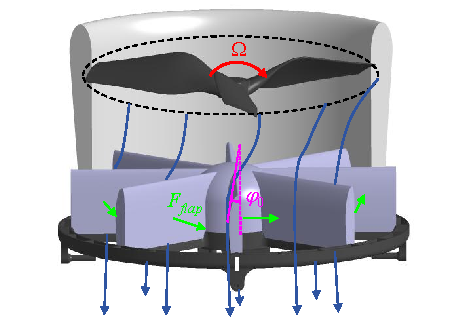
\includegraphics[scale=1]{Fig/固定气动面.pdf}
	\end{minipage}%
    \caption{\label{固定气动面}涵道内部流场示意图}
\end{figure}

经过恰当的设计,固定气动面产生的反扭距$\boldsymbol{M}_{flap}^b$可以抵消大部分的风扇扭矩$\boldsymbol{M}_{fan}^b$。在实践过程中很难达到理想情况,即$\boldsymbol{M}_{flap}^b + \boldsymbol{M}_{fan}^b = \boldsymbol{0}$,所以剩余的力矩部分将由控制舵面的偏置产生偏航力矩来进行补偿。

\section{系统建模总结}

DFUAV的输入变量包括涵道风扇的转速$\Omega$和四个控制舵面的偏转角$\delta_i$,作为动力核心的涵道风扇通过转速调节产生主推力,四片分布式气动舵面通过独立偏转生成三维控制力矩。系统的输出为状态变量,其中包括DFUAV在地面坐标系下的位置$\boldsymbol{P}^{e}=[{x}^{e} \quad {y}^{e} \quad {z}^{e}]^{T}$、地面坐标系下的速度$\boldsymbol{V}^{e}=[{v}^{e}_{x} \quad {v}^{e}_{y} \quad {v}^{e}_{z}]^{T}$、姿态角$\boldsymbol{\eta}=[\varphi \quad \theta \quad \psi]^T$以及机体坐标系下的角速度$\boldsymbol{\omega}^b=[p \quad q \quad r]^T$。结合DFUAV的飞行控制刚体模型和力与力矩的分析,可以推导出DFUAV的非线性动态方程,如下所示:

位置动态方程:
\begin{equation}
    \begin{aligned}
        \dot{x}^{e}&=v_x^e\\
        \dot{y}^{e}&=v_y^e\\
        \dot{z}^{e}&=v_z^e
    \end{aligned}
    \label{eq_40}
\end{equation}

速度动态方程:
\begin{equation}
    \begin{aligned}
        \dot{v}_{x}^{e} & =\frac{1}{m}\Bigg\{ (\cos{\theta}\cos{\psi}) 
        \cdot\left[-\frac{1}{2}\rho C_{D,x}S_xu_r|u_r|+L_x+D_x - V'\rho S u_r + k_\delta V_e^2(\delta_4 - \delta_2)\right] \\
        & \quad+ (\sin{\varphi}\sin{\theta}\cos{\psi}-\cos{\varphi}\sin{\psi}) \\
        & \quad\cdot\left[-\frac{1}{2}\rho C_{D,y}S_yv_r|v_r|+L_y+D_y - V'\rho S v_r + k_\delta V_e^2(\delta_1 - \delta_3)\right] \\
        & \quad+ (\cos{\varphi}\sin{\theta}\cos{\psi}+\sin{\varphi}\sin{\psi}) \\
        & \quad\cdot\left[-k_{fan}\Omega^2-\frac{1}{2}\rho C_{D,z}S_zw_r|w_r|+L_z+D_z\right]
        \Bigg\}
        \\
        \dot{v}_{y}^{e} & =\frac{1}{m}\Bigg\{ (\cos{\theta}\sin{\psi}) \cdot\left[-\frac{1}{2}\rho C_{D,x}S_xu_r|u_r|+L_x+D_x - V'\rho S u_r + k_\delta V_e^2(\delta_4 - \delta_2)\right] \\
        & \quad+ (\sin{\varphi}\sin{\theta}\sin{\psi}+\cos{\varphi}\cos{\psi}) \\
        & \quad\cdot\left[-\frac{1}{2}\rho C_{D,y}S_yv_r|v_r|+L_y+D_y - V'\rho S v_r + k_\delta V_e^2(\delta_1 - \delta_3)\right] \\
        & \quad+ (\cos{\varphi}\sin{\theta}\sin{\psi}-\sin{\varphi}\cos{\psi}) \\
        & \quad\cdot\left[-k_{fan}\Omega^2-\frac{1}{2}\rho C_{D,z}S_zw_r|w_r|+L_z+D_z\right]
        \Bigg\}
        \\
        \dot{v}_{z}^{e} & =\frac{1}{m}\Bigg\{ -\sin{\theta}\cdot\left[-\frac{1}{2}\rho C_{D,x}S_xu_r|u_r|+L_x+D_x - V'\rho S u_r + k_\delta V_e^2(\delta_4 - \delta_2)\right] \\
        & \quad+ (\sin{\varphi}\cos{\theta})\cdot\left[-\frac{1}{2}\rho C_{D,y}S_yv_r|v_r|+L_y+D_y - V'\rho S v_r + k_\delta V_e^2(\delta_1 - \delta_3)\right] \\
        & \quad+ (\cos{\varphi}\cos{\theta}) \cdot\left[-k_{fan}\Omega^2-\frac{1}{2}\rho C_{D,z}S_zw_r|w_r|+L_z+D_z\right]
        \Bigg\}+g
    \end{aligned}
    \label{eq_41}
\end{equation}

欧拉角动态方程:
\begin{equation}
    \begin{aligned}
        \dot{\varphi}&=p+\sin{\varphi}\tan{\theta}q+\cos{\varphi}\tan{\theta}r\\
        \dot{\theta}&=\cos{\varphi}q-\sin{\varphi}r\\
        \dot{\psi}&=\frac{\sin{\varphi}}{\cos{\theta}}q+\frac{\cos{\varphi}}{\cos{\theta}}r
    \end{aligned}
    \label{eq_42}
\end{equation}

角速度动态方程:
\begin{equation}
    \begin{aligned}
        \dot{p}  &=\frac{1}{J_x}\Bigg\{ (J_y-J_z)qr+
        \bigg[\frac{1}{2}\rho{l_a} C_{D,y}S_yv_r|v_r|+L_xl_d+C_{duct}\rho{R}
        v_r|v_r| \bigg.\\
        & \quad\bigg.- l_1k_\delta V_e^2(\delta_1 - \delta_3)-J_{fan}\Omega{q}\bigg]\Bigg\} \\
        \dot{q}  &=\frac{1}{J_y}\Bigg\{ (J_z-J_x)pr+
        \bigg[-\frac{1}{2}\rho{l_a} C_{D,x}S_xu_r|u_r|+L_yl_d+C_{duct}\rho{R}
        u_r|u_r| \bigg.\\
        & \quad\bigg.+ l_1k_\delta V_e^2(\delta_4 - \delta_2)+J_{fan}\Omega{p}\bigg]\Bigg\} \\
        \dot{r}  &=\frac{1}{J_z}\Bigg\{ (J_x-J_y)pq+
        \left[-k_q\Omega^2 +l_2k_\delta V_e^2(\delta_1 + \delta_2 + \delta_3 + \delta_4)\right.\\
        & \quad\left.+V_e^2\varphi_0d_{af}+V_e\Omega{d_{ds}}\right]
        \Bigg\}
    \end{aligned}
    \label{eq_43}
\end{equation}

本文通过物理实验与计算流体力学(Computational Fluid Dynamics,CFD)相结合的方法近似测得试验样机的非线性系统动态方程相关参数,如表\ref{DFUAV_parameters}所示。

\begin{table}
	\caption{\label{DFUAV_parameters}涵道模型参数}
	\centering
	\small 
	\begin{tabular}{cccc}
		\hline 
		参数符号 & 数值                & 参数符号 & 数值                 \tabularnewline
		\hline 
		$m(kg)$   & $1.85$ 		     & $J_x,J_y(kg\cdot{m}^2)$   & $0.0149         $ \tabularnewline
		$J_z(kg\cdot{m}^2)$   & $0.005516$ & $\sigma_d$   & $0.7$ \tabularnewline
        $\rho(kg/m^3)$   & $1.225$ & $R(m)$   & $0.114$ \tabularnewline
        $k_{fan}$   & $9.9796\times10^{-6}$ & $k_q$   & $1.1334\times10^{-7}$ \tabularnewline
        $C_{D,x}$   & $0.43213$ & $C_{D,y}$   & $0.43213$ \tabularnewline
        $C_{D,z}$   & $0.13421$ & $S_x,S_y,S_z(m^2)$   & $0.04$ \tabularnewline
        $l_a(m)$   & $0.1121$ & $C_{duct}$   & $0.78497$ \tabularnewline
        $k_{\delta}$   & $0.0073$ & $J_{fan}(kg\cdot{m}^2)$   & $3.7\times10^{-5}$ \tabularnewline
        $d_{af}$   & $0.01495$ & $d_{ds}$   & $0.01495$ \tabularnewline
        $l_1(m)$   & $0.1708$ & $l_2(m)$   & $0.0066$ \tabularnewline
		\hline 
	\end{tabular}
\end{table}

由DFUAV的非线性动态方程可知,DFUAV的飞行动态呈现为一个高度非线性的多变量耦合系统,系统内各状态变量之间存在着复杂且紧密的相互作用。若要将所有相关变量纳入考量,控制算法的设计工作将尤为棘手。因此在具体实践过程中,可以根据实际情况合力简化模型,有针对性地忽略部分影响较小的因素,保留决定系统宏观特性的主干动力学。然而,模型简化意味着信息缺失,对于未被建模的动态特性(如突然的阵风扰动、机械结构磨损等)以及因简化模型而产生的误差,则可通过鲁棒性的飞行控制算法来进行补偿。

\section{本章小结}

本章主要介绍了试验样机的系统组成并围绕DFUAV的系统建模展开系统性研究。

首先介绍了所使用的试验样机的整体系统组成,明确了各个部分的功能和相互关系,为后续建模及飞行实验奠定物理基础。

接着介绍了坐标系和姿态表示方法,建立了地面坐标系与机体坐标系的转换关系,并根据实际约束采用了‘Z-Y-X’旋转顺序的欧拉角姿态表示方法为飞行控制系统的建模提供了必要的数学分析工具。

在DFUAV的飞行控制刚体模型构建中,结合牛顿-欧拉方程推导出六自由度非线性动力学方程,完整表征平动与转动状态的关系。

并从涵道风扇、机身、涵道翼型、控制舵面和固定气动面等多个方面分析了施加在上面的力与力矩,揭示了各类作用力和控制力矩对飞行器姿态和运动的动态影响。

最后建立了DFUAV的完整的非线性动态方程,本章建立的参数化模型为后续控制算法设计、仿真验证及飞行试验提供了理论框架与数值分析基础。
 % 第二章
\chapter{涵道风扇式无人机的姿态控制}

基于第二章建立的DFUAV非线性系统动态方程分析,其多源力与力矩耦合叠加效应导致姿态动态模型尤为复杂。如滚转角的变化会在俯仰通道和偏航通道上都产生或者间接产生力矩影响,并且三维力矩都与环境风速呈现强相关性。最常用的姿态控制方法基于反馈线性化,比如不考虑系统的数学模型的PID控制算法,虽然该方法面对非线性系统有一定的鲁棒性,但仅通过比例-积分-微分的线性组合应对内外因素产生的力矩影响难免会使系统状态出现超调和滞后等问题。此外,可以使用基于系统模型的方法考虑内外因素对系统状态的影响,但在系统模型参数过多并且不精确的情况下也将为控制算法的设计和系统调试带来很大工作量。基于上述分析,姿态控制算法设计的核心在于如何对难以测得的力矩进行在线补偿。

本章安排如下:首先简要概述增量非线性动态逆控制和控制分配的理论以及二者的结合,然后对DFUAV的姿态动力学模型进行简化处理,方便下文姿态控制算法的设计。接下来给出了基于INDI和优先级控制分配的DFUAV的姿态控制方案设计,最后为验证方案有效性,最后进行了仿真实验和飞行实验验证。

\section{增量非线性动态逆控制与控制分配理论}

NDI(非线性动态逆)是一种基于模型的非线性控制方法,其核心在于在掌握系统模型的情况下,将非线性系统在工作点处进行反馈线性化,然后通过求逆运算来消除系统中的非线性项。当系统模型参数不精确或者对系统机理认识模糊的情况下,NDI方法的控制效果将表现不佳。而INDI(增量式非线性动态逆)相比于NDI采用了增量式的控制策略,仅要求对系统的输入通道建模。INDI在未能充分掌握系统模型的情况下,通过增量式的求逆策略来实时补偿未知扰动与建模误差,得到线性化的系统动力学,进而可以通过常规的线性系统的控制方法来控制\cite{wangStabilityAnalysisIncremental2019b}。因此INDI方法对系统模型的依赖程度较小,是一种基于传感器的方法。此外,INDI方法在设计控制律时主要关注系统的输入输出特性,无需考虑应如何将控制律计算出的控制量分配到各个执行机构上。而后者所描述的任务将由控制分配算法来实现,实现过程中也无需考虑系统内部的复杂非线性因素与动态干扰。因此,采用INDI控制方法有助于将姿态控制算法设计与控制分配算法分离开,实现分层控制。

本节首先将从一般性的系统推导INDI是如何实现增量控制的,然后介绍控制分配理论以及二者的结合。

\subsection{增量非线性动态逆}

考虑如下普通的非线性动力系统:
\begin{align}
    \dot{\boldsymbol{x}}&=\boldsymbol{f}(\boldsymbol{x})+\boldsymbol{g}(\boldsymbol{x},\boldsymbol{u}) \label{3-1}
    \\
    \boldsymbol{y}&=\boldsymbol{h}(\boldsymbol{x})\label{3-2}
\end{align}
上式中$\boldsymbol{x}\in\mathbb{R}^{n}$为n维系统状态变量,$\boldsymbol{u}\in\boldsymbol{U}\in\mathbb{R}^{p}$为p维系统输入变量,其中$\boldsymbol{U}$是容许控制集合,表示对输入变量的约束,$\boldsymbol{y}\in\mathbb{R}^{m}$为m维系统输出变量。映射关系$\boldsymbol{f}:\mathbb{R}^n\rightarrow\mathbb{R}^n$,$\boldsymbol{g}:\mathbb{R}^n\times\mathbb{R}^p\rightarrow\mathbb{R}^n$,$\boldsymbol{h}:\mathbb{R}^n\rightarrow\mathbb{R}^m$。

式\eqref{3-1}中系统状态的一阶泰勒展开式为:
\begin{equation}
    \dot{\boldsymbol{x}}=\dot{\boldsymbol{x}}_0+f^{\prime}(\boldsymbol{x})(\boldsymbol{x}-\boldsymbol{x}_0)+\left.\frac{\partial \boldsymbol{g}}{\partial \boldsymbol{x}}\right|_{\boldsymbol{x}=\boldsymbol{x}_0}(\boldsymbol{x}-\boldsymbol{x}_0)+\left.\frac{\partial \boldsymbol{g}}{\partial \boldsymbol{u}}\right|_{\boldsymbol{u}=\boldsymbol{u}_0}(\boldsymbol{u}-\boldsymbol{u}_0)
    \label{3-3}
\end{equation}
然后对式\eqref{3-2}中的输出表达式求一次导数,结合复合函数求导的链式法则与式\eqref{3-3},可得到动力系统输入与输出之间的关系:
\begin{equation}
    \begin{aligned}
    \dot{\boldsymbol{y}} = \underbrace{\left.\frac{\partial\boldsymbol{h}}{\partial\boldsymbol{x}}\right|_{\boldsymbol{x}=\boldsymbol{x}_0}\dot{\boldsymbol{x}}_0}_{\dot{\boldsymbol{y}}_0} + \left.\frac{\partial \boldsymbol{h}}{\partial \boldsymbol{x}}\right|_{\boldsymbol{x}=\boldsymbol{x}_0}\begin{bmatrix}f^{\prime}(\boldsymbol{x})(\boldsymbol{x}-\boldsymbol{x}_0)+\left.\dfrac{\partial \boldsymbol{g}}{\partial \boldsymbol{x}}\right|_{\boldsymbol{x}=\boldsymbol{x}_0}(\boldsymbol{x}-\boldsymbol{x}_0)+\left.\dfrac{\partial \boldsymbol{g}}{\partial \boldsymbol{u}}\right|_{\boldsymbol{u}=\boldsymbol{u}_0}(\boldsymbol{u}-\boldsymbol{u}_0)\end{bmatrix}
    \end{aligned}
    \label{3-4}
\end{equation}

INDI理论的一个核心假设是时间尺度分离法则\cite{EnergyOptimal},该法则基于系统动力学的时间尺度特性,指出系统内部状态变量的动态响应速率要明显慢于外部输入信号的时变特性。基于这一动力学特性差异,相比于外部输入信号的导数项,系统状态变量的导数项可以视为高阶小量并忽略不计,从而有效地简化系统的动态方程。

基于上述核心假设,可以将式\eqref{3-4}中系统状态的导数项$(\boldsymbol{x}-\boldsymbol{x}_0)$忽略,得到:
\begin{equation}
    \begin{aligned}
    \dot{\boldsymbol{y}} &= \dot{\boldsymbol{y}}_0 +  \left.\frac{\partial \boldsymbol{h}}{\partial \boldsymbol{x}}\right|_{\boldsymbol{x}=\boldsymbol{x}_0}\left.\dfrac{\partial \boldsymbol{g}}{\partial \boldsymbol{u}}\right|_{\boldsymbol{u}=\boldsymbol{u}_0}(\boldsymbol{u}-\boldsymbol{u}_0)\\
        &= \dot{\boldsymbol{y}}_0 + \boldsymbol{G}(\boldsymbol{u}-\boldsymbol{u}_0)
    \end{aligned}
    \label{3-5}
\end{equation}
其中$\dot{\boldsymbol{y}}_0$为系统当前时刻输出的导数,$\boldsymbol{G}\in\mathbb{R}^{m\times p}$,$\boldsymbol{u}_0$为系统当前时刻的控制输入。
使用下标$(.)_{d}$表示该变量的期望值,那么根据公式\eqref{3-5},可以得到期望的输入变量$\boldsymbol{u}_{d}$表示为:
\begin{equation}
    \begin{aligned}
    \boldsymbol{u}_{d}&=\boldsymbol{u}_{0}+\Delta u\\
    &=\boldsymbol{u}_{0}+\boldsymbol{G}^{-1}(\dot{\boldsymbol{y}_d}-\dot{\boldsymbol{y}})
    \label{3-6}
    \end{aligned}
\end{equation}
新的控制输入是在当前时刻的控制输入基础上加上一个控制增量$\Delta u$得到。通过对控制效率矩阵求逆,并且找到期望的输出导数与当前时刻的输出导数的误差,可以得到控制增量。

\subsection{控制分配理论}

继续考虑3.1.1小节中引入的非线性动力系统。对于一个过驱动系统,其系统输入的维度大于系统输出的维度,即$p>m$,表明执行机构存在冗余。将$\boldsymbol{g}(\boldsymbol{x},\boldsymbol{u})$做矩阵分解得到:
\begin{equation}
    \boldsymbol{g}(\boldsymbol{x},\boldsymbol{u})=\boldsymbol{D}\boldsymbol{K}(\boldsymbol{x},\boldsymbol{u})
    \label{3-7}
\end{equation}
其中$\boldsymbol{D}\in\mathbb{R}^{n\times m}$,映射关系$\boldsymbol{K}:\mathbb{R}^n\times\mathbb{R}^p\rightarrow\mathbb{R}^m$。

引入$m$维虚拟控制输入$\boldsymbol{\nu}$:
\begin{equation}
    \boldsymbol{\nu}=\boldsymbol{K}(\boldsymbol{x},\boldsymbol{u})
    \label{3-8}
\end{equation}
由于实际控制输入的约束$\boldsymbol{U}$存在,将实际控制输入变换为虚拟控制输入后有$\boldsymbol{\nu}\in\boldsymbol{\Phi}\in\mathbb{R}^{m}$。容许控制集合$\boldsymbol{U}$通过映射$\boldsymbol{K}$从$\mathbb{R}^{p}$空间映射到$\mathbb{R}^{m}$空间得到可达控制集合$\boldsymbol{\Phi}$,如果$\boldsymbol{\nu}\in\boldsymbol{\Phi}$,则称虚拟控制输入为可达,否则为不可达。虚拟控制输入的物理意义一般为力或力矩。

对$\boldsymbol{\nu}$做一阶泰勒展开并且同样忽略关于系统状态的导数项,得到:
\begin{equation}
    \begin{aligned}
    \boldsymbol{\nu} &= \boldsymbol{\nu}_0 +  \left.\dfrac{\partial \boldsymbol{K}}{\partial \boldsymbol{u}}\right|_{\boldsymbol{u}=\boldsymbol{u}_0}(\boldsymbol{u}-\boldsymbol{u}_0)\\
        &= \boldsymbol{\nu}_0 + \boldsymbol{B}(\boldsymbol{u}-\boldsymbol{u}_0)
    \end{aligned}
    \label{3-9}
\end{equation}
其中$\boldsymbol{\nu}_0$表示系统当前时刻的虚拟控制输入,$\boldsymbol{B}\in\mathbb{R}^{m\times p}$。将$(\boldsymbol{u}-\boldsymbol{u}_0)$代入公式\eqref{3-5},得到:
\begin{equation}
    \begin{aligned}
    \dot{\boldsymbol{y}}=\dot{\boldsymbol{y}}_0+\boldsymbol{G}\boldsymbol{B}^\dagger(\boldsymbol{\nu}-\boldsymbol{\nu}_0)\\
    \Rightarrow \dot{\boldsymbol{y}_d}-\dot{\boldsymbol{y}}_0 = \boldsymbol{G}\boldsymbol{B}^\dagger\Delta\boldsymbol{\nu}
    \label{3-10}
    \end{aligned}
\end{equation}
其中$\boldsymbol{B}^\dagger$表示矩阵$\boldsymbol{B}$的伪逆矩阵,有以下关系:
\begin{gather}
    \boldsymbol{u}=\boldsymbol{B}^\dagger\boldsymbol{\nu}    \label{3-11}
    \\ 
    \boldsymbol{B}^\dagger=\boldsymbol{B}^T\left(\boldsymbol{B}\boldsymbol{B}^T\right)^{-1}    \label{3-12}
\end{gather}

公式\eqref{3-11}中直接表示虚拟控制输入$\boldsymbol{\nu}$与实际控制输入$\boldsymbol{u}$之间映射关系的方法就是伪逆法。在分层控制架构中,系统采用上层决策-底层执行的层级化设计模式:上层控制算法承担决策功能,专注于在线求解系统动力学方程生成期望控制指令,避免了执行机构物理约束对优化问题的干扰,降低了计算复杂度;底层控制分配算法则负责执行任务,采用优化计算方法将上层指令解析为各执行机构的物理控制量,实现控制指令在冗余执行机构中的最优分配。文献\parencite{harkegardResolvingActuatorRedundancy2005}中讨论了层级化设计方法和全阶最优控制设计的联系。采用独立的控制分配算法,优势之一是可以考虑执行机构的物理约束,比如当某个执行机构饱和时,在条件允许的情况下其余执行机构可以用于弥补因该执行机构饱和而损失的控制效能 。图\ref{理论框图}展示了基于INDI的上层控制算法和基于伪逆法的底层控制分配算法的控制系统框图。

\begin{figure}[htbp]
	\centering
	\begin{minipage}[c]{1\textwidth}
		\centering
		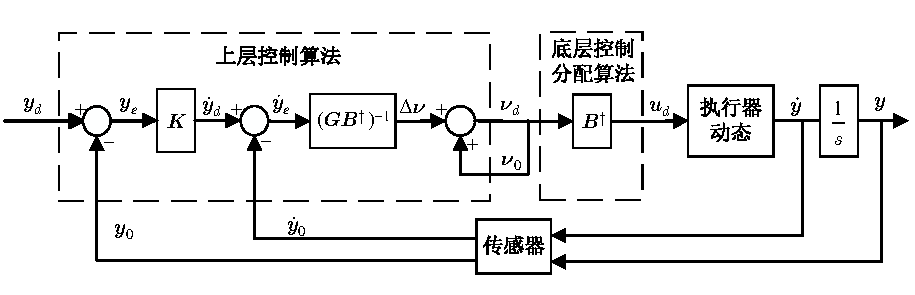
\includegraphics[scale=1]{Fig/理论框图.pdf}
		\caption{\label{理论框图}基于INDI和伪逆法的控制系统框图}
	\end{minipage}%
\end{figure}

需特别指出的是,尽管可以设计出渐进稳定的控制算法,但是受矩阵$\boldsymbol{B}$奇异特性及执行机构物理约束的影响,所推导的期望虚拟控制输入$\boldsymbol{\nu}_d$可能属于不可达集。这一现象在本质上源于伪逆法在控制分配问题中的固有局限性:当控制指令超出执行机构可达包络时,将导致控制分配问题退化为无可行解的数学约束条件,因此下文在控制分配算法的设计中将参考文献\parencite{HKXB202010026},采用优先级控制分配方法。该方法旨在通过优先级排序的方式,优先满足高优先级的控制输入分量以达到更大范围的容许控制。

\section{姿态动力学模型简化}

根据第二章的建模总结可知,DFUAV的姿态动力学模型涉及到多个系统状态变量间的耦合并且与许多模型参数和环境风速有关,尤其是角速度动态方程\eqref{eq_43}中涉及到的多源力矩模型。为便于下文姿态控制算法的设计,本节将对所总结的力矩模型进行合理且适当的简化,根据现有条件区分可控力矩与不可控力矩,然后分别处理。

根据式\ref{eq_11}可知,DFUAV在机体坐标系下的合外力矩可以分解为:
\begin{equation}
    \boldsymbol{M}^b=\boldsymbol{M}_{fan}^b+\boldsymbol{M}_{aero}^b+\boldsymbol{M}_{duct}^b+\boldsymbol{M}_{vane}^b+\boldsymbol{M}_{gyro}^b+\boldsymbol{M}_{flap}^b
    \label{3-13}
\end{equation}
由于涵道风扇的转速$\Omega$可由电调读取,机体的角速度$\boldsymbol\omega^b$可由机载的IMU测量得到,结合表\ref{DFUAV_parameters}中的模型参数,可以计算出涵道风扇的扭矩$\boldsymbol{M}_{fan}^b$和陀螺力矩$\boldsymbol{M}_{gyro}^b$。

模型假设气流相对于机体的速度在$\boldsymbol{O}_b-\boldsymbol{Z}_b$轴的分量为零,即$V_0=0$。根据式\ref{eq_20}以及式\ref{eq_22},可将涵道出口风速$V_{e}$简化为:
\begin{equation}
    V_e=\sqrt{\frac{k_{fan}}{\sigma_d\rho S}}\Omega={k_{f}}\Omega    \label{3-14}
\end{equation}
在这种假设下,涵道出口风速$V_{e}$与风扇转速$\Omega$之间呈正比关系。不妨设$V_e=k_{f}\Omega$,其中$k_{f}=\sqrt{\frac{k_{fan}}{\sigma_d\rho S}}$可以根据表\ref{DFUAV_parameters}中的参数计算得到。然后根据控制舵面的偏转角$\delta_{i}$和涵道力臂的长度,可计算出控制舵面产生的力矩$\boldsymbol{M}_{vane}^b$。

对于在固定气动面上产生的反扭距$\boldsymbol{M}_{flap}^b$,由于$V_{e}$与$\Omega$为正比关系,可将式\ref{eq_39}简化为:
\begin{equation}
    \boldsymbol{M}_{flap}^b=
    \begin{bmatrix}
    0 \\0 \\k_{flap}\Omega^2
    \end{bmatrix}
    \label{3-15}
\end{equation}

现在考虑风扇扭矩$\boldsymbol{M}_{fan}^b$、固定气动面上的反扭距$\boldsymbol{M}_{flap}^b$和控制舵面在$\boldsymbol{O}_b-\boldsymbol{Z}_b$轴的偏航力矩。根据第二章的力矩分析,仅有上述三部分分量会对机体的偏航力矩产生影响。为使机体的偏航角保持稳定,有如下关系:
\begin{equation}
    \begin{gathered}
    -k_q\Omega^2+k_{flap}\Omega^2+k_{\delta}k_f^2 l_2(\delta_1 + \delta_2 + \delta_3 + \delta_4)\Omega^2=0
     \\
     \Rightarrow
    -k_q+k_{flap}+k_{\delta}k_f^2 l_2(\delta_1 + \delta_2 + \delta_3 + \delta_4)=0
    \end{gathered}
    \label{3-16}
\end{equation}
式\ref{3-15}中等式约去风扇转速变量$\Omega$后,只有控制舵面的偏转角是变量,其他均为确定的模型参数。这表明了当机体偏航角稳定时,所需的控制舵面偏转角是一定的。由于$k_{flap}$与固定气动面的设计形状有关,不失一般性,本文假设固定气动面在恰当的设计下可以使得$k_{flap}=k_{q}$,即:
\begin{equation}
    \boldsymbol{M}_{flap}^b + \boldsymbol{M}_{fan}^b = \boldsymbol{0}
\label{3-17}
\end{equation}

对于在机身上产生的气动力矩$\boldsymbol{M}_{aero}^b$和由于涵道翼型产生的力矩$\boldsymbol{M}_{duct}^b$,由于机体相对于气流的速度$\boldsymbol{V}_a^b$在现有条件下是未知的,所以将其视为不可控力矩来作为未建模动态力矩。使用$\boldsymbol{M}_{a}^b$统一表示:
\begin{equation}
    \boldsymbol{M}_{a}^b=\boldsymbol{M}_{aero}^b+\boldsymbol{M}_{duct}^b
    \label{3-18}
\end{equation}

$\boldsymbol{M}_{a}^b$可以描述为地面坐标系下的速度$\boldsymbol{V}^e$、姿态$\boldsymbol{\eta}$和环境风速$\boldsymbol{W}^e$的函数,即:
\begin{equation}
    \boldsymbol{M}_{a}^b=\boldsymbol{M}_{a}^b(\boldsymbol{V}^e,\boldsymbol{\eta},\boldsymbol{W}^e)
    \label{3-19}
\end{equation}

综合以上分析,简化后的气动力矩模型可以写为:
\begin{equation}
    \boldsymbol{M}^b=\boldsymbol{M}_{vane}^b+\boldsymbol{M}_{gyro}^b+\boldsymbol{M}_{a}^b
    \label{3-20}
\end{equation}
与力矩模型相关的角速度动态方程对应的可以简写为:
\begin{equation}
    \begin{aligned}
        \dot{p}  &=\frac{1}{J_x}\Bigg\{ (J_y-J_z)qr+
        \big[- l_1k_\delta V_e^2(\delta_1 - \delta_3)-J_{fan}\Omega{q} +\boldsymbol{M}_{ax}^b\big]\Bigg\} \\
        \dot{q}  &=\frac{1}{J_y}\Bigg\{ (J_z-J_x)pr+
        \big[l_1k_\delta V_e^2(\delta_4 - \delta_2)+J_{fan}\Omega{p} +\boldsymbol{M}_{ay}^b\big]\Bigg\} \\
        \dot{r}  &=\frac{1}{J_z}\Bigg\{ (J_x-J_y)pq+
        \left[l_2k_\delta V_e^2(\delta_1 + \delta_2 + \delta_3 + \delta_4) + \boldsymbol{M}_{az}^b\right]
        \Bigg\}
    \end{aligned}
    \label{3-21}
\end{equation}
上述简化的力矩模型将可控力矩与不可控力矩分开。控制舵面合力矩$\boldsymbol{M}_{vane}^b$作为可控力矩由下文设计的姿态控制算法来计算期望力矩(即期望的控制舵面偏转角度)。陀螺力矩$\boldsymbol{M}_{gyro}^b$同样作为可控力矩,但该力矩会对DFUAV的姿态造成负面影响,下文将根据其产生的机理设计对应的陀螺力矩补偿算法加以补偿。而$\boldsymbol{M}_{a}^b$作为不可控力矩将通过姿态控制算法在在线补偿。

\section{基于INDI和优先级控制分配的姿态控制方案}

根据本章开篇时的分析,姿态控制算法设计的核心在于如何对难以测得的力矩进行在线补偿。在第二节姿态动力学模型简化中,将难以测得的力矩视为了未建模动态力矩$\boldsymbol{M}_{a}^b$。基于INDI的控制架构设计,其优势主要体现在模型的鲁棒性与未建模误差的动态补偿能力。式\eqref{3-21}中的形式已十分适用于INDI姿态控制器的设计:一方面,姿态子系统的输入通道的模型机理已经明确,由四片独立的控制舵面产生偏转角作为输入信号;另一方面,由于未建模动态力矩$\boldsymbol{M}_{a}^b$作用于角加速度,所以可用机载IMU高频测量角速度并估算角加速度,并根据INDI的增量式求逆策略在线补偿未建模动态力矩$\boldsymbol{M}_{a}^b$。在所构建的控制架构中,控制输入分为两部分:INDI输入与反馈输入。INDI输入针对$\boldsymbol{M}_{a}^b$进行补偿,将非线性系统转化为线性形式;而反馈输入针对此线性形式设计反馈控制律,保证系统的稳定性和鲁棒性。

根据优先级控制分配的思想,需要将控制输入分量进行优先级排序。由于INDI输入包含对未建模动态力矩的补偿,反馈输入使用线性的状态反馈设计,与系统响应相关。系统能够稳定运行的前提是首先消除未建模动态力矩的影响,将非线性系统化为线性系统,然后再设计反馈控制律,确保系统的稳定性与响应能力。因此本文中将INDI输入视为高优先级分量,反馈输入视为低优先级分量。确保INDI输入不会产生分配误差,在控制舵面受到物理约束的情况下仅在反馈输入中产生分配误差。具体而言,这种划分方法可以在一定程度上避免系统输出耦合现象\cite{HKXB202010026}。

\subsection{INDI姿态控制架构}

对于大部分无人机姿态运动控制,常采用基于欧拉角参数化的局部线性化方法,滚转角、俯仰角和偏航角三个通道分别作为控制目标单独控制,使得无人机的旋转过程被线性化处理。但是不同于位置动态方程\eqref{eq_40},欧拉角动态方程\eqref{eq_42}将三个姿态通道耦合在一起。实际上,无人机的姿态属于$SO(3)$上的流形结构,任何姿态变化都被视为流形上的测地线运动。而传统的局部线性化跟踪姿态的方法相当于在流形的切空间进行局部线性逼近,这种线性化处理方式导致了姿态轨迹生成过程中的不连续性,丢失了流形的曲率信息,所以在机动飞行时会导致姿态跟踪误差变大。因此本文参考文献\parencite{10.1115/1.4052714}在$SO(3)$上考虑姿态误差的表示。

由于旋转矩阵$\boldsymbol{R}\in{SO(3)}$,姿态欧拉角$\boldsymbol{\eta}\in\mathbb{R}^3$,因此定义符号$[.]_\times$表示映射关系$\mathbb{R}^3\to SO(3)$,$(.)^\vee$表示对应的逆映射$SO(3)\to\mathbb{R}^3$。对于任意姿态$\boldsymbol{\eta}=[\varphi \quad \theta \quad \psi]^T$,对应的矩阵形式可以表示为:
\begin{equation}
    \boldsymbol{R}=[\boldsymbol{\eta}]_\times=
    \begin{bmatrix}
    0 & -\psi & \theta \\
    \psi & 0 & -\varphi \\
    -\theta & \varphi & 0
    \end{bmatrix}
    \label{3-22}
\end{equation}

假设期望姿态为$\boldsymbol{\eta}_d$,当前姿态为$\boldsymbol{\eta}$,对应的矩阵形式分别为$\boldsymbol{R}_d$和$\boldsymbol{R}$。则在${SO(3)}$上的姿态误差可以表示为:
\begin{equation}
    \boldsymbol{e}_R=\dfrac{1}{2}(\boldsymbol{R}_d^T\boldsymbol{R}-\boldsymbol{R}^T\boldsymbol{R}_d)^\vee\in \mathbb{R}^3
    \label{3-23}
\end{equation}

因此期望的姿态欧拉角变化率可以表示为:
\begin{equation}
    \dot{\boldsymbol{\eta}}_1=-\boldsymbol{K}_R\boldsymbol{e}_R
    \label{3-24}
\end{equation}
其中$\boldsymbol{K}_R=diag({K}_{R\varphi},{K}_{R\theta},{K}_{R\psi})$为姿态误差的正定增益矩阵。式\eqref{3-24}所示的作差方式类似于于反馈信号减去给定信号,所以需要加负号。

为提高系统的响应速度,确保快速跟踪期望姿态,引入前馈控制策略:
\begin{equation}
    \dot{\boldsymbol{\eta}}_2=\frac{d\boldsymbol{\eta}_d}{dt}
    \label{3-25}
\end{equation}

结合式\eqref{eq_10}、式\eqref{3-24}和式\eqref{3-25},期望的机体角速度$\boldsymbol\omega^{b}_d$可以表示为:
\begin{equation}
    \boldsymbol{\omega}^{b}_d=\boldsymbol{Q}^{-1}( \dot{\boldsymbol{\eta}}_1+ \dot{\boldsymbol{\eta}}_2)
    \label{3-26}
\end{equation}

接下来考虑与动力学相关的角速度动态,包含了可控力矩与不可控力矩。如前文所述,DFUAV姿态子系统的控制输入为四片相互独立的控制舵面的偏转角$\delta_i$,由四个偏转角度的组合产生用于控制机体姿态的俯仰力矩、滚转力矩和偏航力矩,因此姿态子系统中存在执行机构的冗余,存在过驱动的问题。引入虚拟控制输入$\boldsymbol{\nu}\in\mathbb{R}^3$将姿态控制算法与控制分配算法分开:
\begin{equation}
    \boldsymbol{\nu}=
    \begin{bmatrix}
    {\nu}_x \\ {\nu}_y \\ {\nu}_z
    \end{bmatrix}=\boldsymbol{B}
    \begin{bmatrix}
    \delta_1 \\ \delta_2 \\ \delta_3 \\ \delta_4
    \end{bmatrix}
    \label{3-27}
\end{equation}
其中矩阵$\boldsymbol{B}$表示四片独立控制舵面偏转角到三维虚拟控制输入的映射矩阵,有$\boldsymbol{B}\in\mathbb{R}^{3\times4}$。

结合式\eqref{eq_10}、式\eqref{eq_36}、式\eqref{3-14}和式\eqref{3-27},可以将可控的控制舵面力矩重写为模块化形式:
\begin{equation}
    (\boldsymbol{J}^b)^{-1}\boldsymbol{M}_{vane}^b=\boldsymbol{H}_{vane}\boldsymbol{\nu}\Omega^2
    \label{3-28}
\end{equation}
其中
\begin{gather}
\left.\boldsymbol{H}_{vane}\triangleq k_{\delta}k_f^2\left[
    \begin{array}
    {ccc}2J_x^{-1}l_1 & & \\
        & 2J_y^{-1}l_1 & \\
        & & 4J_z^{-1}l_2
    \end{array}\right.\right]\in\mathbb{R}^{3\times3}
    \label{3-29}\\
    \boldsymbol{B}=
    \begin{bmatrix}
    -0.5 & 0 & 0.5 & 0 \\
    0 & -0.5 & 0 & 0.5 \\
    0.25 & 0.25 & 0.25 & 0.25
    \end{bmatrix}
    \label{3-30}
\end{gather}
经过式\eqref{3-28}的模块化处理,由原本的从控制舵面角度到控制力矩的映射转变为了从控制舵面角度到虚拟控制输入的映射。在此过程中,映射矩阵剔除了所有与模型相关参数项。

对于可控的陀螺力矩$\boldsymbol{M}_{gyro}^b$,根据式\eqref{eq_10}和式\ref{eq_38},可将其模块化表示为:
\begin{equation}
    (\boldsymbol{J}^b)^{-1}\boldsymbol{M}_{gyro}^b=\boldsymbol{H}_{gyro}(\boldsymbol{\omega}^b)\Omega
    \label{3-31}
\end{equation}
其中
\begin{equation}
    \boldsymbol{H}_{gyro}(\boldsymbol{\omega}^b) \triangleq J_{fan}[-J_x^{-1}q\quad J_y^{-1}p\quad0]^T\in\mathbb{R}^{3}
    \label{3-32}
\end{equation}

对于不可控的气动力矩$\boldsymbol{M}_{a}^b$,将其与式\eqref{eq_10}中的非线性项$(\boldsymbol{J}^b\boldsymbol{\omega}^b\times\boldsymbol{\omega}^b)$一同处理,表示为与地面坐标系下的速度$\boldsymbol{V}^e$、姿态$\boldsymbol{\eta}$、环境风速$\boldsymbol{W}^e$和机体角速度$\boldsymbol{\omega}^b$有关的函数:
\begin{equation}
    ({\boldsymbol{J}^b})^{-1}(\boldsymbol{M}_{a}^b+\boldsymbol{J}\boldsymbol{\omega}^b\times\boldsymbol{\omega}^b)\triangleq \boldsymbol{L}(\boldsymbol{V}^e,\boldsymbol{\eta},\boldsymbol{W}^e,\boldsymbol{\omega}^b)\in\mathbb{R}^3
    \label{3-33}
\end{equation}

结合式\eqref{3-28}、式\eqref{3-31}和式\eqref{3-33},角速度动态方程可以被模块化表示为:
\begin{equation}
    \boldsymbol{\dot{\omega}}^b=\boldsymbol{H}_{vane}\boldsymbol{\nu}\Omega^2+\boldsymbol{H}_{gyro}(\boldsymbol{\omega}^b)\Omega+\boldsymbol{L}(\boldsymbol{V}^e,\boldsymbol{\eta},\boldsymbol{W}^e,\boldsymbol{\omega}^b)
    \label{3-34}
\end{equation}
可以直接在该模型的基础上应用INDI,而无需考虑控制分配问题。根据本章第一节介绍的INDI理论,为了得到$\boldsymbol{\dot{\omega}}^b$的增量表达式,对公式\eqref{3-34}在其工作点处(使用下标$(.)_0$表示)作一阶泰勒展开:
\begin{equation}
    \begin{aligned}
    \boldsymbol{\dot{\omega}}^b&=\boldsymbol{H}_{vane}\boldsymbol{\nu}\Omega^2+\boldsymbol{H}_{gyro}(\boldsymbol{\omega}^b)\Omega+\boldsymbol{L}(\boldsymbol{V}^e,\boldsymbol{\eta},\boldsymbol{W}^e,\boldsymbol{\omega}^b)\\
    &=\boldsymbol{H}_{vane}\boldsymbol{\nu}_0\Omega_0^2+\boldsymbol{H}_{gyro}(\boldsymbol{\omega}_0^b)\Omega_0+\boldsymbol{L}_0\\
    & +\left.\frac{\partial(\boldsymbol{H}_{vane}\boldsymbol{\nu}\Omega^2)}{\partial\boldsymbol{\nu}}\right|_{\boldsymbol{\nu}=\boldsymbol{\nu}_0}(\boldsymbol{\nu}-\boldsymbol{\nu}_0)
    +\left.\bigg[\frac{\partial(\boldsymbol{H}_{vane}\boldsymbol{\nu}\Omega^2)}{\partial\Omega}+\frac{\partial(\boldsymbol{H}_{gyro}\Omega)}{\partial\Omega}\bigg]\right|_{\Omega=\Omega_0}
    (\Omega-\Omega_0) \\
     & +\left.\bigg[\frac{\partial(\boldsymbol{H}_{gyro}\Omega)}{\partial\boldsymbol{\omega}^{b}}+\frac{\partial\boldsymbol{L}}{\partial\boldsymbol{\omega}^{b}}\bigg]\right|_{\boldsymbol{\omega}^{b}=\boldsymbol{\omega}_{0}^{b}}(\boldsymbol{\omega}^{b}-\boldsymbol{\omega}_{0}^{b})\\
    & +\left.\frac{\partial\boldsymbol{L}}{\partial\boldsymbol{V}^{e}}\right|_{\boldsymbol{V}^{e}=\boldsymbol{V}_{0}^{e}}
    (\boldsymbol{V}^{e}-\boldsymbol{V}_{0}^{e})
    +\left.\frac{\partial\boldsymbol{L}}{\partial\boldsymbol{\eta}}\right|_{\boldsymbol{\eta}=\boldsymbol{\eta}_{0}}(\boldsymbol{\eta}-\boldsymbol{\eta}_{0})
    +\left. \frac{\partial\boldsymbol{L}}{\partial\boldsymbol{W}^e}\right|_{\boldsymbol{W}^e=\boldsymbol{W}_0{}^e}(\boldsymbol{W}^e-\boldsymbol{W}_0{}^e)
    \end{aligned}
    \label{3-35}
\end{equation}
展开式中的第一项$\boldsymbol{H}_{vane}\boldsymbol{\nu}_0\Omega_0^2+\boldsymbol{H}_{gyro}(\boldsymbol{\omega}_0^b)\Omega_0+\boldsymbol{L}_0$等价于工作点处的角加速度,可以由机载IMU测量的角速度经过差分滤波得到:
\begin{equation}
    \boldsymbol{\dot{\omega}}^b_0=\boldsymbol{H}_{vane}\boldsymbol{\nu}_0\Omega_0^2+\boldsymbol{H}_{gyro}(\boldsymbol{\omega}_0^b)\Omega_0+\boldsymbol{L}_0
    \label{3-36}
\end{equation}

展开式中的其他项是关于系统内部状态变量$(\boldsymbol{V}^e,\boldsymbol{\eta},\boldsymbol{\omega}^b)$、系统控制输入$(\boldsymbol{\nu},\Omega)$和外部扰动$\boldsymbol{W^e}$的一阶偏导数项。根据本章第一小节介绍的时间尺度分离法则,认为在角加速度的输入信号的时间尺度内,系统内部状态变量包括速度、姿态和机体角速度的变化是缓慢的,因此可以将这些状态变量的一阶偏导数项视为0:
\begin{equation}
    \begin{cases}
        \boldsymbol{V}^e-\boldsymbol{V}_0^e\approx0 \\
        \boldsymbol{\eta}-\boldsymbol{\eta}_0\approx0 \\
        \boldsymbol{\omega}^b-\boldsymbol{\omega}_0^b\approx0
    \end{cases}
    \label{3-37}
\end{equation}

在无人机控制中,执行机构(如电机、舵机等)可在数十毫秒的时间尺度内完成控制指令的执行,产生所需的力与力矩。而机体的速度、姿态等状态变量受空气动力阻尼、质量惯性等因素的制约,其动态过程一般落后于执行机构响应1-2个数量级,因此上述假设是合理的。此外,对于外部环境风速扰动$\boldsymbol{W}^e$的变化是未知并且难以预测的,因此假定$(\boldsymbol{W}^e-\boldsymbol{W}_0^e\approx0)$。但此假设并没有排除外部环境风速扰动对系统的影响,缓慢变化的自然风对姿态造成的影响已被考虑在$\boldsymbol{L}_0$中。而应对快速变化的风速扰动则取决于所设计的姿态控制器的鲁棒性。

其余关于系统控制输入的偏导数项如下:
\begin{equation}
    \begin{gathered}
    \left.\frac{\partial(\boldsymbol{H}_{vane}\boldsymbol{\nu}\Omega^2)}{\partial\boldsymbol{\nu}}\right|_{\boldsymbol{\nu}=\boldsymbol{\nu}_0}(\boldsymbol{\nu}-\boldsymbol{\nu}_0)=\boldsymbol{H}_{vane}\Omega_0^2(\boldsymbol{\nu}-\boldsymbol{\nu}_0) \\
    \left.\bigg[\frac{\partial(\boldsymbol{H}_{vane}\boldsymbol{\nu}\Omega^2)}{\partial\Omega}+\frac{\partial(\boldsymbol{H}_{gyro}\Omega)}{\partial\Omega}\bigg]\right|_{\Omega=\Omega_0}(\Omega-\Omega_0)=\big[2\boldsymbol{H}_{vane}\boldsymbol{\nu}_0\Omega_0+\boldsymbol{H}_{gyro}(\boldsymbol{\omega}_0^b)\big](\Omega-\Omega_0)
    \end{gathered}
    \label{3-38}
\end{equation}

因此,角速度动态的一阶泰勒展开式\eqref{3-35}近似可以表示为:
\begin{equation}
    \boldsymbol{\dot{\omega}}^b=\boldsymbol{\dot{\omega}}_0^b+\boldsymbol{H}_{vane}\Omega_0^2(\boldsymbol{\nu}-\boldsymbol{\nu}_0)+\big[2\boldsymbol{H}_{vane}\boldsymbol{\nu}_0\Omega_0+\boldsymbol{H}_{gyro}(\boldsymbol{\omega}_0^b)\big](\Omega-\Omega_0)
    \label{3-39}
\end{equation}

值得一提的是,风扇转速$\Omega$作为速度控制的输入信号并不直接参与姿态控制。简化后的角速度动态(即式\eqref{3-21})中与$\Omega$相关的项均与陀螺力矩$\boldsymbol{M}_{gyro}^b$有关,将由下文设计的陀螺力矩补偿算法补偿。因此$\Omega$不被视为姿态控制中输入信号的一部分,可以将$\Omega$作为在角速度动态中的已知参数,该参数可以从速度环设计中得到。为了简便表示,采用以下记号:
\begin{equation}
    \boldsymbol{T}(\Omega)=\big[2\boldsymbol{H}_{vane}\boldsymbol{\nu}_0\Omega_0+\boldsymbol{H}_{gyro}(\boldsymbol{\omega}_0^b)\big](\Omega-\Omega_0)\in\mathbb{R}^3
    \label{3-40}
\end{equation}

将式\eqref{3-40}代入式\eqref{3-39},可以得到角速度$\boldsymbol{\omega}^b$动态的增量表达式:
\begin{equation}
    \begin{aligned}
    \boldsymbol{\dot{\omega}}^b&=\boldsymbol{\dot{\omega}}_0^b+\boldsymbol{H}_{vane}\Omega_0^2(\boldsymbol{\nu}-\boldsymbol{\nu}_0)+\boldsymbol{T}(\Omega)\\
    &=\begin{bmatrix}\dot{p}_0 \\ \dot{q}_0 \\ \dot{r}_0 \end{bmatrix}
    + k_{\delta}k_f^2\Omega_0^2
    \left[\begin{array}{ccc}2J_x^{-1}l_1 & & \\& 2J_y^{-1}l_1 & \\& & 4J_z^{-1}l_2\end{array}\right]
    \left(\begin{bmatrix}\nu_{x} \\ \nu_{y} \\ \nu_{z}\end{bmatrix}
    -\begin{bmatrix}\nu_{x0} \\ \nu_{y0} \\ \nu_{z0}\end{bmatrix}\right)
    +  \begin{bmatrix}T_{x}(\Omega) \\ T_{y}(\Omega) \\ T_{z}(\Omega)
    \end{bmatrix}
    \end{aligned}
    \label{3-41}
\end{equation}

INDI通过对式\eqref{3-41}进行求逆,来得到期望的虚拟控制输入的增量表达式:
\begin{equation}
    \begin{aligned}
        \boldsymbol{\nu}_d&=(\boldsymbol{H}_{vane}\Omega_0^2)^{-1}\Big\{\boldsymbol{\mu} -\big[\boldsymbol{\dot{\omega}}_0^b+\boldsymbol{T}(\Omega_d)\big]\Big\}+\boldsymbol{\nu}_0\\
        &=\frac{1}{k_{\delta}k_f^2\Omega_0^2}
        \left[\begin{array}{ccc}2J_x^{-1}l_1 & & \\& 2J_y^{-1}l_1 & \\& & 4J_z^{-1}l_2\end{array}\right]^{-1}
        \left\{\begin{bmatrix}\mu_{x} \\ \mu_{y} \\ \mu_{z}\end{bmatrix}
        -\left (\begin{bmatrix}\dot{p}_0 \\ \dot{q}_0 \\ \dot{r}_0 \end{bmatrix}+\begin{bmatrix}T_{x}(\Omega_d) \\ T_{y}(\Omega_d) \\ T_{z}(\Omega_d)
        \end{bmatrix}\right )\right\}
        +  \begin{bmatrix}\nu_{x0} \\ \nu_{y0} \\ \nu_{z0}\end{bmatrix}
    \end{aligned}
    \label{3-42}
\end{equation}
其中,虚拟输入项$\boldsymbol{\nu}$被$\boldsymbol{\nu}_d$替换,表明是期望的输入。类似地,$\boldsymbol{\Omega}$被替换为$\boldsymbol{\Omega}_d$。

将式\eqref{3-42}代入式\eqref{3-41},得到线性化的角速度动态方程:
\begin{equation}
    \dot{\boldsymbol \omega}^b=\boldsymbol{\mu}
    \label{3-43}
\end{equation}

最终,通过以下比例反馈律,可以得到稳定的角速度子系统:
\begin{equation}
    \boldsymbol{\mu}=\boldsymbol{K}_{\omega}(\boldsymbol{\omega}_d^b-\boldsymbol{\omega}^b)
    \label{3-44}
\end{equation}

将式\eqref{3-44}代入式\eqref{3-43}中可以得到:
\begin{equation}
    \dot{\boldsymbol \omega}^b=\boldsymbol{K}_{\omega}(\boldsymbol{\omega}_d^b-\boldsymbol{\omega}^b)
    \label{3-45}
\end{equation}
其中$\boldsymbol{K}_\omega=diag({K}_{\omega p},{K}_{\omega q},{K}_{\omega r})$为正反馈增益矩阵。

基于INDI的控制思想已经把非线性角速度动力学方程\eqref{3-34}简化为了一个一阶积分系统\eqref{3-43},因此采用单一的比例控制器就可以确保闭环系统的稳定性,只需要保证反馈增益为正,而不管其具体取值。这进一步提供了一个指导,可以分别确定闭环系统的静态平衡点和动态性能。因此结合式\eqref{3-44},可以将式\eqref{3-42}可以分为两部分:
\begin{equation}
    \boldsymbol{\nu}_d=\boldsymbol{\nu}_i + \boldsymbol{\nu}_f
    \label{3-46}
\end{equation}
其中$\boldsymbol{\nu}_i$定义为INDI输入,$\boldsymbol{\nu}_f$定义为反馈输入,具体形式为:
\begin{equation}
    \begin{aligned}
        \boldsymbol{\nu}_i&=-(\boldsymbol{H}_{vane}\Omega_0^2)^{-1} \big[\boldsymbol{\dot{\omega}}_0^b+\boldsymbol{T}(\Omega_d)\big]+\boldsymbol{\nu}_0\\
        &=-\frac{1}{k_{\delta}k_f^2\Omega_0^2}
        \left[\begin{array}{ccc}2J_x^{-1}l_1 & & \\& 2J_y^{-1}l_1 & \\& & 4J_z^{-1}l_2\end{array}\right]^{-1}
        \left (\begin{bmatrix}\dot{p}_0 \\ \dot{q}_0 \\ \dot{r}_0 \end{bmatrix}+\begin{bmatrix}T_{x}(\Omega_d) \\ T_{y}(\Omega_d) \\ T_{z}(\Omega_d)
        \end{bmatrix}\right )
        +  \begin{bmatrix}\nu_{x0} \\ \nu_{y0} \\ \nu_{z0}\end{bmatrix}
    \end{aligned}
    \label{3-47}
\end{equation}
\begin{equation}
    \begin{aligned}
        \boldsymbol{\nu}_f&=(\boldsymbol{H}_{vane}\Omega_0^2)^{-1}\boldsymbol{K}_{\omega}(\boldsymbol{\omega}_d^b-\boldsymbol{\omega}^b)\\
        &=\frac{1}{k_{\delta}k_f^2\Omega_0^2}
        \left[\begin{array}{ccc}2J_x^{-1}l_1 & & \\& 2J_y^{-1}l_1 & \\& & 4J_z^{-1}l_2\end{array}\right]^{-1}
        \left[\begin{array}{ccc}{K}_{\omega p} & & \\& {K}_{\omega q} & \\& & {K}_{\omega r}\end{array}\right]
        \left (\begin{bmatrix}\dot{p}_d \\ \dot{q}_d \\ \dot{r}_d \end{bmatrix}-\begin{bmatrix}\dot{p} \\ \dot{q} \\ \dot{r}
        \end{bmatrix}\right )
    \end{aligned}
    \label{3-48}
\end{equation}

INDI采用增量控制策略,将未建模动态力矩项$\boldsymbol{M}_{a}^b$和角速度动力学耦合项$\boldsymbol{J}\boldsymbol{\omega}^b\times\boldsymbol{\omega}^b$造成的影响放在了$\dot {\boldsymbol{\omega}}_0^b$中处理。在每一个工作点计算的INDI输入都是基于上一个工作点的INDI输入加上模型误差、阵风扰动以及风扇转速输入对相邻两个工作点之间的角加速度影响。因此,模型误差不会随着时间进行累计,而是在每一个工作点实时补偿。而系统的稳定性由基于误差的角速度反馈来保证。

根据上述分析,INDI输入的计算依赖于机体的角加速度值$\dot {\boldsymbol{\omega}}_0^b$,在现有条件下,该值可以通过对机体陀螺仪测量的相邻两个采样点的角速度进行一阶差分得到:
\begin{equation}
    \dot{\boldsymbol{\omega}}^b(k)=\frac{
        \begin{bmatrix}
        \boldsymbol{\omega}^b(k)-\boldsymbol{\omega}^b(k-1)
        \end{bmatrix}}{\Delta t}
    \label{3-49}
\end{equation}
其中$\Delta t$是陀螺仪传感器的采样时间,$k$为传感器的采样点,泰勒展开式中的工作点一般选取为当前的采样时刻。因此INDI也被称为基于传感器的方法。

在飞行控制系统的工程实现中,为了提高姿态控制器的响应速度和控制精度,$\Delta t$应该在条件允许的情况下尽可能小。但是传感器测量得到的角速度原始值会受到机体震动和外部扰动等因素的影响,难免会有噪声,对原始值进行差分运算后会放大这种噪声的影响,采样时间越小,噪声影响越大。因此在实际应用中,需要对角速度进行滤波处理。但是滤波处理就会在角加速度的计算中引入延迟,由于INDI是将角速度动力学方程在工作点处进行一阶泰勒展开,所以需要保证展开式\eqref{3-41}中所有下标为0的项都位于同一工作点。一种方法是对角加速度进行预测,如采用卡尔曼滤波器对其进行预测来补偿相位滞后,但是这种方法需要对角加速度进行额外的建模,并且角速度收到的的干扰也无法预测。或者采用多个加速度计数据融合来直接测量角加速度,但是这种方式会导致机载航电系统设计过于复杂,并且加速度计受机体震动影响也较大,多传感器数据融合的精度难以有效保证。

因此,本文针对所有下标为0的项进行同步滤波处理,除了角加速度项外,还包括虚拟控制输入项和风扇转速输入项。文献\parencite{smeurAdaptiveIncrementalNonlinear2015,smeurCascadedIncrementalNonlinear2018b}通过四旋翼飞行实验表明这种处理方式的可行性。考虑到陀螺仪传感器的高频噪声影响,本文实验使用的滤波器是二阶巴特沃斯(Butterworth)低通滤波器,滤波器截止频率的具体数值应该根据飞行过程中信号的频率成分、带宽和噪声水平来综合确定。对于本文使用的DFUAV,滤波器截止频率为30Hz。为加以区分,所有下标为0的项经过滤波器滤波后,使用下标$(.)_s$表示。

\subsection{陀螺力矩补偿}

在基于INDI的控制架构中,陀螺力矩$\boldsymbol{M}_{gyro}^b$分量蕴含在了$\boldsymbol{T}(\Omega)$中(见式\eqref{3-40}),该力矩的存在会在姿态发生改变时影响姿态跟踪精度。因此,为了消除陀螺力矩对姿态控制的影响,需要在INDI输入$\boldsymbol{\nu}_i$中对其进行补偿。由于姿态子系统的控制输入为控制舵面的偏转角度,并且根据式\eqref{eq_38}可知陀螺力矩的机理已十分明确。所以可以将陀螺力矩对应的值等价转化为虚拟控制输入量,然后在$\boldsymbol{\nu}_i$中减去该分量,即可对陀螺力矩造成的负面影响进行补偿。

根据式\eqref{eq_35}、\eqref{eq_36}和式\eqref{3-14},在现有条件下可用于计算的控制舵面力矩可表示为:
\begin{gather}
    \boldsymbol{M}_{vane}^b=k_{\delta}k_f^2\Omega^2\begin{bmatrix}
        -l_1 & 0 & l_1 & 0 \\
        0 & -l_1 & 0 & l_1 \\
        l_2 & l_2 & l_2 & l_2
        \end{bmatrix}\boldsymbol{{\delta}}
    \label{3-50}
\end{gather}

将式\eqref{3-27}代入式\eqref{3-50}可得:
\begin{gather}
    \boldsymbol{M}_{vane}^b=k_{\delta}k_f^2\Omega^2\begin{bmatrix}
        -l_1 & 0 & l_1 & 0 \\
        0 & -l_1 & 0 & l_1 \\
        l_2 & l_2 & l_2 & l_2
        \end{bmatrix}\boldsymbol{B}^{\dagger}\boldsymbol{\nu}
    \label{3-51}
\end{gather}
根据式\eqref{3-12}以及式\eqref{3-30}中矩阵B的值,可以计算得到$\boldsymbol{B}^{\dagger}$为:
\begin{gather}
    \boldsymbol{B}^{\dagger}=
        \begin{bmatrix}
        -1 & 0 & 1 \\
        0 & -1 & 1  \\
        1 & 0 & 1 \\
        0 & 1 & 1
        \end{bmatrix}
    \label{3-52}
\end{gather}

如果直接计算与陀螺力矩等效的控制舵面的偏转角度,那么就有可能在在实际控制中出现控制舵面的偏转角度超过其可行范围的情况。这是因为与陀螺力矩等效的控制舵面的偏转角度未经过控制分配算法的优化分配,导致期望的控制效果与实际不符。因此,此处计算与陀螺力矩等效的虚拟控制输入以便于INDI输入$\boldsymbol{\nu}_i$一起参与优先级控制分配。

令式\eqref{eq_38}所描述的陀螺力矩和式\eqref{3-51}描述的控制舵面力矩相等,可以得到与陀螺力矩等效的虚拟控制输入$\boldsymbol{\nu}_{gyro}$:
\begin{equation}
    \begin{gathered}
        \boldsymbol{M}_{gyro}^b=\boldsymbol{M}_{vane}^b\\
        \Rightarrow J_{fan}\Omega\begin{bmatrix}-q \\ p \\ 0\end{bmatrix}
        =
        k_{\delta}k_f^2\Omega^2\begin{bmatrix}
            -l_1 & 0 & l_1 & 0 \\
            0 & -l_1 & 0 & l_1 \\
            l_2 & l_2 & l_2 & l_2
            \end{bmatrix}\boldsymbol{B}^{\dagger}\boldsymbol{\nu}_{gyro}\\
        \Rightarrow \boldsymbol{\nu}_{gyro}=\frac{J_{fan}}{k_{\delta}k_f^2\Omega}\boldsymbol{B}\begin{bmatrix}
            -l_1 & 0 & l_1 & 0 \\
            0 & -l_1 & 0 & l_1 \\
            l_2 & l_2 & l_2 & l_2
            \end{bmatrix}^{\dagger}\begin{bmatrix}-q \\ p \\ 0\end{bmatrix}
        \label{3-53}
    \end{gathered}
\end{equation}

因此,加入陀螺力矩补偿后的INDI输入$\boldsymbol{\nu}_i$为:
\begin{equation}
    \begin{aligned}
        \boldsymbol{\nu}_i&=-(\boldsymbol{H}_{vane}\Omega_0^2)^{-1} \big[\boldsymbol{\dot{\omega}}_0^b+\boldsymbol{T}(\Omega_d)\big]+\boldsymbol{\nu}_0-\boldsymbol{\nu}_{gyro}
    \end{aligned}
    \label{3-54}
\end{equation}
其中$\boldsymbol{\nu}_{gyro}$表达式中的风扇转速项$\Omega$和角速度项$\boldsymbol{\omega}^b$都需要同步滤波。

\subsection{优先级控制分配}

由于DFUAV的特殊构型,飞行过程中由期望控制输入计算出的控制舵面偏转角很可能超出其物理约束,所以底层设计用于解决控制分配问题。该问题可以描述为对于给定的三维期望虚拟控制输入$\boldsymbol{\nu}_d$,找到一组四片控制舵面的偏转角度在容许控制集合的范围内$\boldsymbol{\delta}_d\in \boldsymbol{U}$使得$\boldsymbol{\nu}_d=\boldsymbol{B}\boldsymbol{\delta}_d$,或者在无法找到这样一组解的情况下,需要找到一组最优解使得分配误差$\boldsymbol{\nu}_d-\boldsymbol{B}\boldsymbol{\delta}_d$最小化。容许控制集合$\boldsymbol{U}$由下式定义:
\begin{equation}
    \boldsymbol{U}=\{\boldsymbol{\delta}\in\mathbb{R}^4|-\delta_m\leq\delta_i\leq\delta_m,i=1,2,3,4\}
    \label{3-55}
\end{equation}

对应的,虚拟控制输入$\boldsymbol{\nu}$的可达集合$\boldsymbol\Phi$表示为:
\begin{equation}
    \boldsymbol\Phi=\left\{\boldsymbol{\nu}\in\mathbb{R}^3|\boldsymbol{\nu}=\boldsymbol{B}\boldsymbol{\delta},\boldsymbol{\delta}\in \boldsymbol{U}\right\}
    \label{3-56}
\end{equation}
其中$\boldsymbol{B}$由式\eqref{3-30}给出。

为了实现控制分配的目标,广泛采用的方法是直接计算矩阵$\boldsymbol{B}$的伪逆矩阵$\boldsymbol{B}^{\dagger}$,然后计算$\boldsymbol{\delta}_d$:
\begin{equation}
    \boldsymbol{\delta}_d=\boldsymbol{B}^{\dagger}\boldsymbol{\nu}_d
    \label{3-57}
\end{equation}

使用伪逆方法的优点是计算简单,易于理解。但是在工作点的约束边界区,即使$\boldsymbol{\nu}_d$保持在可达集合内,伪逆法计算出的$\boldsymbol{\delta}_d$中的部分分量也可能会超出约束边界,即$\boldsymbol{\delta}\notin\boldsymbol{U}$。在这种情况下,伪逆法会计算出一个基于某种性能指标的次最优解,次最优解可能有多种选择,所以次最优解之间亦有优劣之分。伪逆法没有对这些解进行优先级排序,因此无法保证次最优解的唯一性。

为了弥补伪逆方法的不足,采用优先级控制分配方法,将期望的虚拟控制输入进行矢量分解划分各自的优先级,优先满足高优先级的控制输入分量。式\eqref{3-46}已将期望的虚拟控制输入$\boldsymbol{\nu}_d$分为两部分,即$\boldsymbol{\nu}_i$和$\boldsymbol{\nu}_f$,其中$\boldsymbol{\nu}_i$是INDI输入,$\boldsymbol{\nu}_f$是反馈输入。根据本节开篇时的分析,为优先补偿系统的非线性未建模动态力矩,视$\boldsymbol{\nu}_i$为高优先级控制输入分量,而$\boldsymbol{\nu}_f$为低优先级控制输入分量。考虑到控制舵面的物理约束,期望的虚拟控制输入应该被限制在其可达集合内。在本文中,假设在适当的外部扰动下,无人机运动过程中总能满足高优先级分量的可达。即:
\begin{equation}
    \boldsymbol{\nu}_i\in\boldsymbol\Phi
    \label{3-58}
\end{equation}
如果由于控制舵面的饱和而使得$\boldsymbol{\nu}_i$超出可达集合,那么姿态将不受控制,闭环系统失去可控性。但是这种情况不在本文的讨论范围内。

由于总的虚拟控制输入$\boldsymbol{\nu}_d$是受到可达集合限制的,并且INDI输入分量$\boldsymbol{\nu}_i$假定总是可达的。这表明了总的虚拟控制输入中的另一部分分量,即反馈输入分量$\boldsymbol{\nu}_f$,可能会超出可达集合的范围,因此需要对$\boldsymbol{\nu}_f$进行约束。使用比例因子$\alpha$将$\boldsymbol{\nu}_f$限制在可达集合内,即:
\begin{equation}
    \boldsymbol{\nu}_d=\boldsymbol{\nu}_i+\alpha\boldsymbol{\nu}_f,\quad\text{其中}0\leq\alpha\leq1
    \label{3-59}
\end{equation}
因为$\dot{\boldsymbol{\omega}}^b$仍由式\eqref{3-45}控制,所以保持$\boldsymbol{\nu}_i$不变并对$\boldsymbol{\nu}_f$进行缩放只会影响闭环系统的动态性能,而不会影响闭环系统的稳定性。

当虚拟控制输入可达时,比例因子$\alpha$等于1,此时的优先级控制分配方法等价于伪逆法。当虚拟控制输入不可达时,比例因子$\alpha$小于1,表明对低优先级分量$\boldsymbol{\nu}_f$进行截断,保证了高优先级分量$\boldsymbol{\nu}_i$的可达性。

综上所述,优先级控制分配算法可以通过解决以下线性优化问题来实现对高优先级分量的保持和低优先级分量的截断:
\begin{equation}
    \begin{gathered}
        \max_{\alpha,\boldsymbol{\delta}}\alpha \\
        \text{subject  to}
        \begin{cases}
        \boldsymbol{\delta}\in\boldsymbol{U} \\
        \boldsymbol{B}\boldsymbol{\delta}=\boldsymbol{\nu}_i+\alpha\boldsymbol{\nu}_f \\
        0\leq\alpha\leq1
        \end{cases}
    \end{gathered}
    \label{3-60}
\end{equation}

在具体实践过程中,上述线性优化问题通过以下步骤进行求解:首先判断给定的$\boldsymbol{\nu}_d=\boldsymbol{\nu}_i+\boldsymbol{\nu}_f$是否可达,即$\alpha$等于1的情况。如果可达,直接使用伪逆法计算$\boldsymbol{\delta}_d$并返回最优解;如果不可达,即$0\leqslant\alpha<1$,则可以使用单纯形法通过基变量变换逐步迭代逼近最优解。首先通过以下公式满足高优先级分量$\boldsymbol{\nu}_i$:
\begin{equation}
    \boldsymbol{\nu}_i=\boldsymbol{B}\boldsymbol{\delta}^\prime,\quad\boldsymbol{\delta}^\prime=[\delta_{1}^\prime\quad\delta_{2}^\prime\quad\delta_{3}^\prime\quad\delta_{4}^\prime]^T\in\boldsymbol{U}
    \label{3-61}
\end{equation}

如果$\boldsymbol{\nu}_i$不可达,则直接返回$\boldsymbol{\delta}_d=\boldsymbol{\delta}^\prime$。否则$\boldsymbol{\nu}_i$可达,接下来需要满足低优先级分量$\boldsymbol{\nu}_f$,此时容许控制集合变为:
\begin{equation}
    \boldsymbol{U}^\prime=\{\boldsymbol{\delta}\in\mathbb{R}^4|-\delta_m-\delta_{i}^\prime\leq\delta_i\leq\delta_m-\delta_{i}^\prime,i=1,2,3,4\}
    \label{3-62}
\end{equation}

可以通过下式计算低优先级分量对应的舵面偏转:
\begin{equation}
    \boldsymbol{\nu}_f=\boldsymbol{B}\boldsymbol{\delta}^{\prime\prime},\quad\boldsymbol{\delta}^{\prime\prime}=[\delta_{1}^{\prime\prime}\quad\delta_{2}^{\prime\prime}\quad\delta_{3}^{\prime\prime}\quad\delta_{4}^{\prime\prime}]^T\in\boldsymbol{U}^{\prime}
    \label{3-63}
\end{equation}

最终得到期望舵面偏转角为:
\begin{equation}
    \boldsymbol{\delta}_d = \boldsymbol{\delta}^{\prime}+\boldsymbol{\delta}^{\prime\prime}
    \label{3-64}
\end{equation}

式\eqref{3-60}的优化结果能够保证对于每一个由上层姿态控制算法计算出的期望虚拟控制输入,都有:
\begin{equation}
    \boldsymbol{\nu}_d=\boldsymbol{\nu}_i+\alpha\boldsymbol{\nu}_f\in \boldsymbol{\Phi}
\label{3-65}
\end{equation}
这保证了$\boldsymbol{\nu}_d$的可达性以及次最优解的唯一性,区别仅是$\alpha$的取值不同。

值得注意的是,上述分解方式是人为规定的,在具体实践过程中还可以根据场景需求作其他种类的分解,比如定义分量的优先级和定义分解的维度等。除了INDI方法外,其他的控制方法包括串级PID控制律、ADRC控制律\cite{HKXB202010026}等都可以针对虚拟控制输入进行矢量分解。

图\ref{实际框图}所示的控制系统框图展示了上层设计采用INDI姿态控制方法,底层设计采用优先级控制分配方法的分层控制架构。
\begin{figure}[htbp]
	\centering
	\begin{minipage}[c]{1\textwidth}
		\centering
		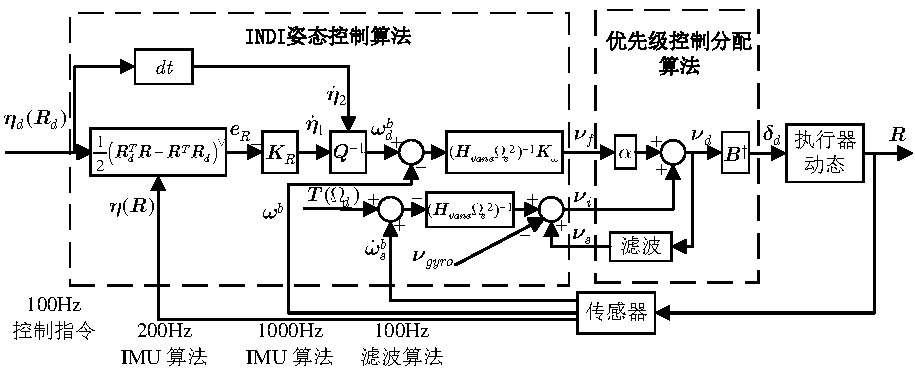
\includegraphics[scale=1]{Fig/实际框图.pdf}
		\caption{\label{实际框图}基于INDI和优先级控制分配法的姿态控制系统框图}
	\end{minipage}%
\end{figure}

\section{实验和结果分析}

为了验证提出的基于上层INDI+底层优先级控制分配的姿态控制方法的性能,本小节进行了一系列仿真实验与实际飞行实验,包括INDI姿态控制方法对比串级PID姿态控制方法和优先级控制分配方法对比伪逆方法。作为对照实验的串级PID控制方法中,角度环采用单一的P控制器,角速度环采用PI控制器。实验过程中使用的INDI姿态控制器和串级PID姿态控制器的参数如下表\ref{Control_parameters}所示,$\boldsymbol{K}_{R}$表示角度环比例增益,$\boldsymbol{K}_{\omega}$表示角速度环比例增益,$\boldsymbol{I}_{\omega}$表示角速度环积分增益。为了保证实验过程中其他条件的一致性,在INDI控制对比PID控制的实验过程中,底层控制分配方法都采用伪逆法。而在优先级控制分配方法对比伪逆方法的实验过程中,上层姿态控制均采用INDI方法。
\begin{table}
	\caption{\label{Control_parameters}INDI控制器和PID控制器的各项参数}
	\centering
	\small 
	\begin{tabular}{cccccc}
		\hline 
		INDI控制器参数符号 & 数值 & PID控制器参数符号 & 数值 & PID控制器参数符号 & 数值 \tabularnewline
		\hline 
		$K_{R\varphi}$ & $5.5$ & $K_{R\varphi}$ & $5.5 $& $I_{\omega p}$ & $0.1$ \tabularnewline
		$K_{R\theta}$   & $5.5$ & $K_{R\theta}$   & $5.5$& $I_{\omega q}$   & $0.1$ \tabularnewline
        $K_{R\psi}$   & $5.0$ & $K_{R\psi}$   & $5.0$& $I_{\omega r}$   & $0.1$ \tabularnewline
        $K_{\omega p}$   & $0.3$ & $K_{\omega p}$   & $0.3$ \tabularnewline
        $K_{\omega q}$   & $0.3$ & $K_{\omega q}$   & $0.3$ \tabularnewline
        $K_{\omega r}$   & $0.18$ & $K_{\omega r}$   & $0.18$ \tabularnewline
		\hline 
	\end{tabular}
\end{table}

仿真实验平台为MATLAB,DFUAV的仿真模型相关参数参考表\ref{DFUAV_parameters},仿真模型中采用基于龙格-库塔(Runge-Kutta)法的ode45数值求解器求解DFUAV的非线性动态方程(式\eqref{eq_10})。实际飞行实验平台使用2.1节介绍的试验样机。为了提高数据的一致性并且减少风扇转速$\Omega$变化带来的耦合效应,需要保证姿态控制过程中的高度稳定,因此实验中采用了位置控制器,该控制器的设计方法将于第四章具体介绍。应当注意的是,位置控制器的加入并不影响姿态控制器的性能验证。悬停时风扇的旋转速度约为7639转/分钟。

为了体现所提出的姿态控制器的抗干扰性能,本文设计了一种主动产生扰动的方案。由于姿态动力学系统的输入信号为控制舵面的偏转角度,所以实验中通过在一些控制舵面上添加固定的偏置来引入干扰,如图\ref{主动扰动}所示。此外,为了防止因加入固定偏置而导致控制舵面饱和的问题,当添加固定偏置时,对应控制舵面的最大偏转角度也应该同步调整。调整时也需要确保控制算法在正负方向上响应的对称性。例如在1号控制舵面上添加了$5^{\circ}$的固定偏置,那么1号控制舵面的最大偏转角度应该限制为$\pm(\delta_m-5^{\circ})$,即$\pm35^{\circ}$,其他舵面的最大偏转角度保持$\pm40^{\circ}$不变。

\begin{figure}[htbp]
	\centering
        \subfloat[INDI对比PID的扰动设置]
		{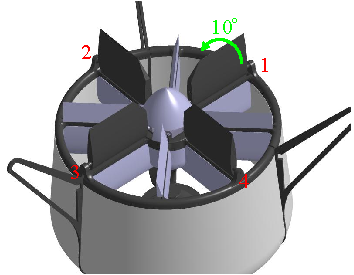
\includegraphics[scale=1]{Fig/主动扰动1.pdf}
		\label{实验一扰动}}
        \subfloat[优先级控制分配对比伪逆的扰动设置]
        {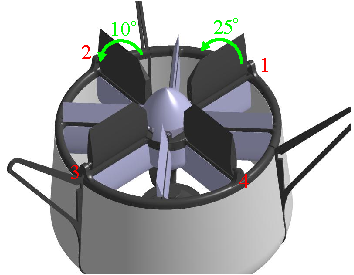
\includegraphics[scale=1]{Fig/主动扰动2.pdf}
		\label{实验二扰动}}
    \caption{主动扰动实验设置}\label{主动扰动}
\end{figure}

\subsection{仿真实验}

\subsubsection{INDI对比PID}

本实验的目的是验证在MATLAB仿真环境中搭建的INDI控制器在有无干扰情况下的性能,采用PID姿态控制器作为实验对比。扰动的添加方式如图\ref{实验一扰动}所示,在1号控制舵面上添加$10^{\circ}$的固定偏置,这会在机体上产生额外的负滚转力矩和正偏航力矩,1号舵的偏转角度限幅被同时调整为$\pm30^{\circ}$。实验总时长为6s,仿真步长为0.01s。仅在滚转通道设置方波指令信号,俯仰和偏航通道的指令均设置为0。

没有添加扰动时的实验对比结果如图\ref{INDI对比PID仿真无扰动}所示。根据实验结果可知,在滚转通道上,INDI控制和PID控制都可以及时地跟踪期望姿态指令,但是相比于PID控制,INDI控制器的超调量相对较小,并且收敛速度更快。对于俯仰和偏航通道,添加了陀螺力矩补偿的INDI控制器在滚转姿态变化时能够更好地抑制陀螺力矩的影响,从而提高了姿态控制的精度。
\begin{figure}[htbp]
	\centering
	\begin{minipage}[c]{1\textwidth}
        \centering
        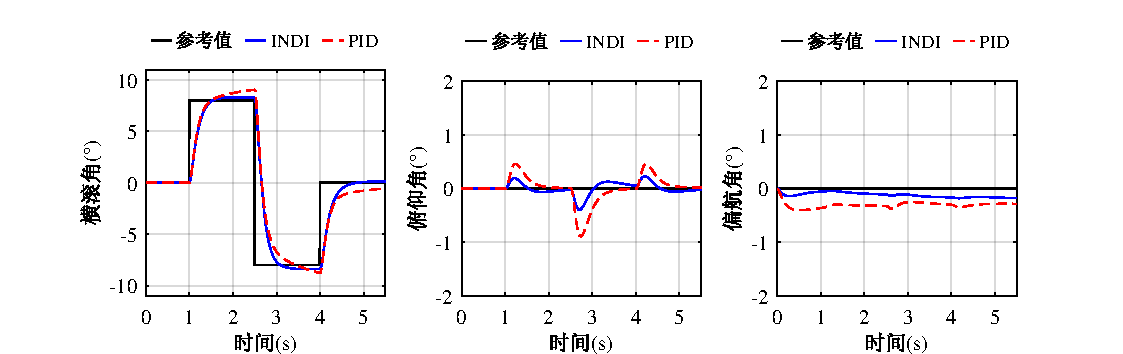
\includegraphics[scale=1]{Fig/INDI对比PID无扰动仿真实验结果.pdf}
        \caption{\label{INDI对比PID仿真无扰动}INDI对比PID在无扰动情况下的仿真实验结果}
        \end{minipage}
\end{figure}

添加干扰情况下的实验对比结果如图\ref{INDI对比PID仿真有扰动}所示,扰动在方波输入时同步添加。在滚转通道上,INDI控制器在添加扰动后仍然能够保持较好的跟踪性能,似乎与未添加扰动情况下的姿态响应曲线没有区别,这是由于INDI控制器能够补偿未建模动态力矩$\boldsymbol{M}_a^b$,并且在每一个控制周期内都会实时补偿而不会积累误差。但是PID控制器依赖误差才能修正,存在未知扰动的情况下由于无法及时预测和补偿误差,所以表现出了明显的滞后与超调量,并且在INDI控制下的姿态达到稳态时,PID控制下的姿态仍存在明显的偏差。在偏航通道上,INDI对于扰动引起的偏航力矩的抑制能力同样明显优于PID。
\begin{figure}[htbp]
	\centering
	\begin{minipage}[c]{1\textwidth}
        \centering
        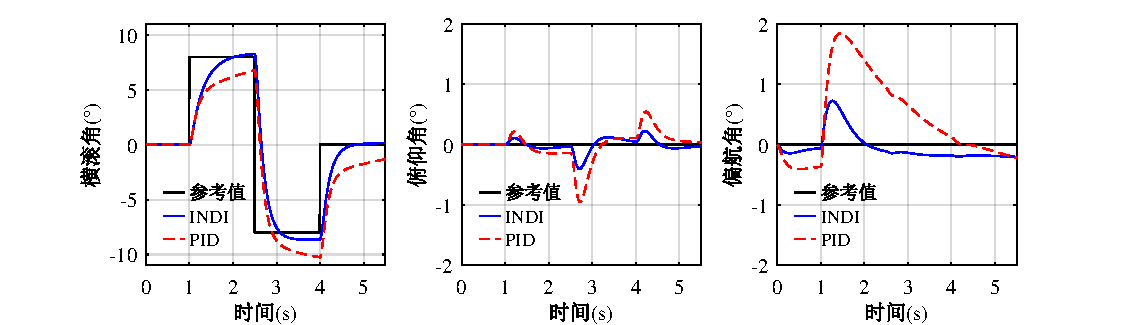
\includegraphics[scale=1]{Fig/INDI对比PID有扰动仿真实验结果.pdf}
        \caption{\label{INDI对比PID仿真有扰动}INDI对比PID在有扰动情况下的仿真实验结果}
        \end{minipage}
\end{figure}

\subsubsection{优先级控制分配对比伪逆}

本实验用于验证设计的优先级控制分配算法在控制舵面饱和情况下的有效性,对比实验为前文提到的伪逆方法。扰动的添加方式如图\ref{实验二扰动}所示,在1号控制舵面上添加$25^{\circ}$的固定偏置,并且在2号控制舵面上添加$10^{\circ}$的固定偏置,这会在机体上产生额外的负滚转力矩、负俯仰力矩和正偏航力矩。1号舵的偏转角度限幅被同时调整为$\pm15^{\circ}$,2号舵的偏转角度限幅被同时调整为$\pm30^{\circ}$。实验总时长为2s,仿真步长为0.01s。为了便于观察三个通道受扰动影响的情况,三个姿态通道的参考指令均设置为0,扰动在第1s时刻添加。

姿态通道的实验结果如图\ref{优先级伪逆姿态仿真}所示。可以看出,三个姿态通道的误差变化情况都与扰动产生的力矩的变化情况相一致。但是以优先级控制分配算法作为底层分配算法时的姿态通道误差幅值明显比伪逆法更小,这是由于优先级控制分配算法优先满足了高优先级分量$\boldsymbol{\nu}_i$,使执行机构的变化能够及时地补偿未建模动态力矩的影响。这也说明了本文的划分优先级分量思路的正确性。
\begin{figure}[htbp]
	\centering
	\begin{minipage}[c]{1\textwidth}
        \centering
        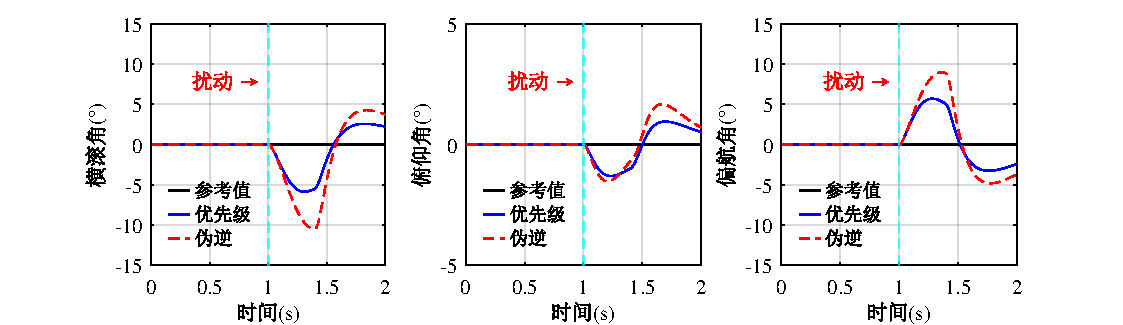
\includegraphics[scale=1]{Fig/优先级对比伪逆的姿态保持仿真实验结果.pdf}
        \caption{\label{优先级伪逆姿态仿真}优先级控制分配对比伪逆法的姿态保持仿真实验结果}
        \end{minipage}
\end{figure}

另一种可以直观感受控制分配方法优劣的方式是比较分配误差。伪逆方法的分配误差定义为:
\begin{equation}
    \boldsymbol{e}_{pinv}=\boldsymbol{\nu}_d-\boldsymbol{B}\boldsymbol{\delta}_d
    \label{3-66}
\end{equation}
其中$\boldsymbol{\delta}_d$是通过式\eqref{3-57}计算得到的,该值需要被限制在容许控制集合$\boldsymbol{U}$内。

优先级控制分配算法的分配误差定义为$\boldsymbol{e}_{i}+\boldsymbol{e}_{f}$,两个分量分别表示INDI分配误差和反馈分配误差。可以通过下式计算:
\begin{equation}
    \begin{gathered}
        \begin{cases}
            \boldsymbol{e}_{i}=\boldsymbol{\nu}_i-\boldsymbol{B}\boldsymbol{\delta}^{\prime} \\
            \boldsymbol{e}_{f}=\boldsymbol{\nu}_f-\boldsymbol{B}\boldsymbol{\delta}^{\prime\prime}
        \end{cases}
    \end{gathered}
    \label{3-67}
\end{equation}
其中$\boldsymbol{\delta}^{\prime}$可以由式\eqref{3-61}计算得到,$\boldsymbol{\delta}^{\prime\prime}$可以由式\eqref{3-63}计算得到。

两种分配方法对应的分配误差如图\ref{优先级伪逆分配误差仿真}所示。可以看出,扰动添加的瞬间立刻在三个通道上产生分配误差。但是优先级控制分配算法的分配误差在扰动添加之后的短暂时间内迅速减小,而伪逆方法的分配误差则是不断增大一段时间才减小,且分配误差的幅值也明显大于优先级控制分配算法。说明本文使用的优先级控制分配算法提高了姿态控制的精度。
\begin{figure}[htbp]
	\centering
	\begin{minipage}[c]{1\textwidth}
        \centering
        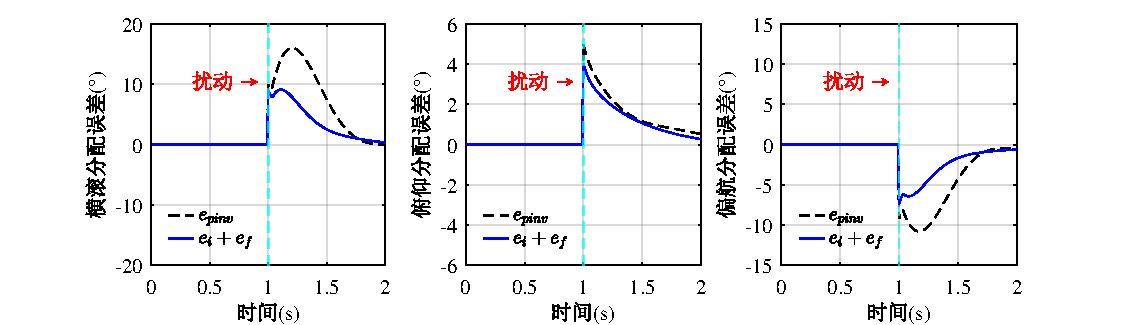
\includegraphics[scale=1]{Fig/优先级对比伪逆的分配误差仿真实验结果.pdf}
        \caption{\label{优先级伪逆分配误差仿真}优先级控制分配对比伪逆法的分配误差仿真实验结果}
        \end{minipage}
\end{figure}

图\ref{优先级分量分配误差仿真}展示了仿真实验中优先级分量各自对应的分配误差$\boldsymbol{e}_i$和$\boldsymbol{e}_f$的比较。从图中可以明显的看出INDI分配误差$\boldsymbol{e}_i$始终保持为零,这表明分量$\boldsymbol{\nu}_i$在实验过程中始终满足可达性约束,这是因为INDI输入分量位于高优先级,分配算法将优先满足该分量。而优先级控制分配的分配误差全由反馈分配误差$\boldsymbol{e}_f$贡献,这表明了优先级控制分配算法由于控制舵面的饱和对反馈输入进行了截断。通过仿真实验验证了优先级控制分配算法的可行性和有效性。
\begin{figure}[htbp]
	\centering
	\begin{minipage}[c]{1\textwidth}
        \centering
        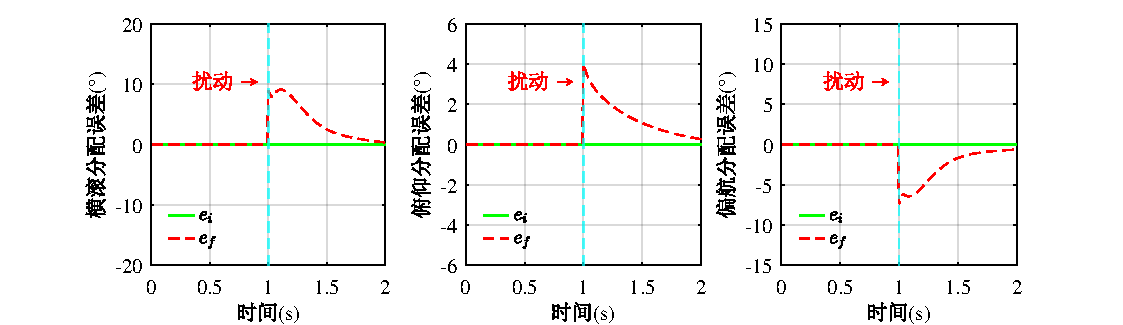
\includegraphics[scale=1]{Fig/优先级各分量的分配误差仿真实验结果.pdf}
        \caption{\label{优先级分量分配误差仿真}优先级分量各自的分配误差仿真实验结果}
        \end{minipage}
\end{figure}
\subsection{实际飞行实验}

\subsubsection{INDI对比PID}

本实验的目的是使用第二章介绍的试验样机验证提出的基于INDI的姿态控制器在实际飞行中是否能够稳定的跟踪期望姿态以及抵抗外部干扰的能力。实验过程同样分为无扰动和有扰动两种情况。实验条件的设计与仿真实验中保持一致,包括扰动的添加方式(见图\ref{实验一扰动})和方波指令的输入等。实际控制器的步长为0.01s。

无扰动和有扰动情况下的姿态控制实际飞行实验结果分别如图\ref{INDI对比PID无扰动飞行实验结果}和图\ref{INDI对比PID有扰动飞行实验结果}所示。从实验结果可以看出,在实际飞行情况下,INDI姿态控制器跟踪期望姿态的能力同样优于PID姿态控制器。相比PID,INDI在滚转通道的超调量更小,上升时间更短,在俯仰和偏航通道上的姿态误差也更小。结果与仿真实验中相符。

在添加干扰的情况下,INDI姿态控制器同样也表现出了更好的抗干扰能力,跟踪误差较小。而PID控制器则难以有效应对外部干扰,表现出了较大的跟踪误差。这进一步验证了INDI控制器在实际飞行中的有效性。
\begin{figure}[htbp]
	\centering
	\begin{minipage}[c]{1\textwidth}
        \centering
        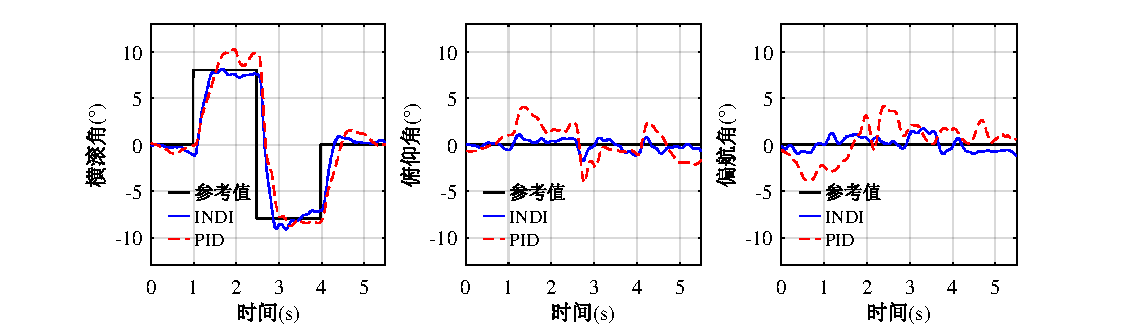
\includegraphics[scale=1]{Fig/INDI对比PID无扰动飞行实验结果.pdf}
        \caption{\label{INDI对比PID无扰动飞行实验结果}INDI对比PID无扰动时的飞行实验结果}
        \end{minipage}
\end{figure}
\begin{figure}[htbp]
	\centering
	\begin{minipage}[c]{1\textwidth}
        \centering
        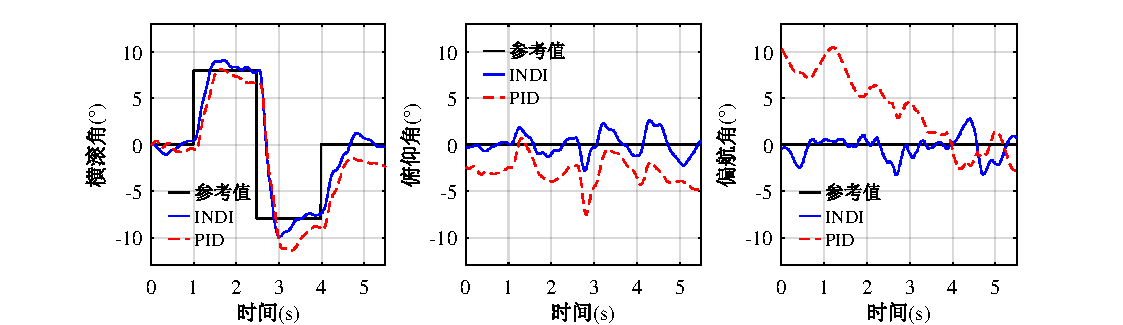
\includegraphics[scale=1]{Fig/INDI对比PID有扰动飞行实验结果.pdf}
        \caption{\label{INDI对比PID有扰动飞行实验结果}INDI对比PID有扰动时的飞行实验结果}
        \end{minipage}
\end{figure}

\subsubsection{优先级控制分配对比伪逆}

本实验用于验证设计的优先级控制分配算法在实际飞行过程中的表现情况。实验条件的设计与仿真实验中保持一致,扰动的添加方式采用图\ref{实验二扰动}中的设计,三轴期望姿态都被设置为0。对照实验采用伪逆法,两种分配算法的执行步长均为0.01s。

姿态通道的实际飞行实验结果如图\ref{优先级对比伪逆的姿态保持飞行实验结果}所示。三轴的姿态误差变化情况与主动扰动产生的力矩变化情况相一致。但是在优先级控制分配算法下,三轴姿态通道的姿态误差幅值更小,并且误差收敛的速度也更快。上述结果与仿真实验中保持一致,进一步说明了仿真实验中结果分析的正确性。
\begin{figure}[htbp]
	\centering
	\begin{minipage}[c]{1\textwidth}
        \centering
        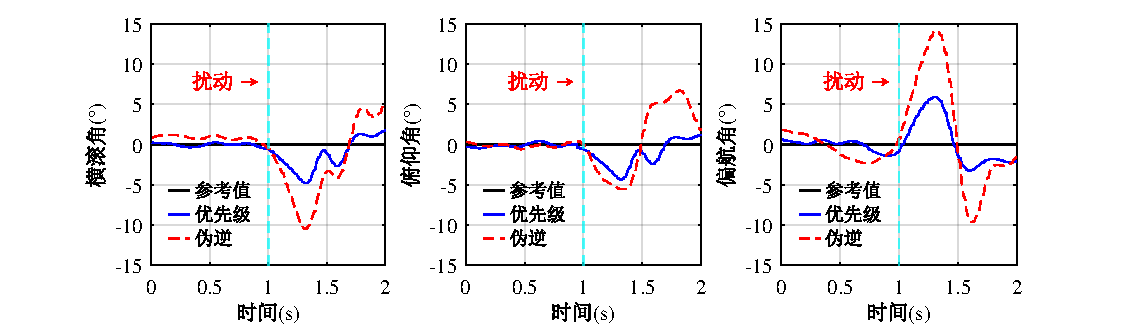
\includegraphics[scale=1]{Fig/优先级对比伪逆的姿态保持飞行实验结果.pdf}
        \caption{\label{优先级对比伪逆的姿态保持飞行实验结果}优先级对比伪逆的姿态保持飞行实验结果}
        \end{minipage}
\end{figure}

两种分配方法的分配误差的比较如图\ref{优先级对比伪逆的分配误差飞行实验结果}所示。分配误差于式\eqref{3-66}和式\eqref{3-67}中定义。从图中可以看出,伪逆方法下的总体分配误差远大于优先级控制分配算法下的分配误差,这导致了伪逆方法下的姿态误差也更大。这说明本文设计的优先级控制分配算法在实际飞行中同样能够提高姿态控制的精度。

实际飞行实验中优先级分量的分配误差比较如图\ref{优先级各分量的分配误差飞行实验结果}所示。从图中可以看出,即使是在实际飞行中,INDI输入分量$\boldsymbol{\nu}_i$也始终满足可达性约束。反馈分配误差$\boldsymbol{e}_i$的存在表明优先级控制分配算法对$\boldsymbol{\nu}_f$进行了截断。通过实际飞行实验进一步验证了优先级控制分配算法的可行性和有效性。
\begin{figure}[htbp]
	\centering
	\begin{minipage}[c]{1\textwidth}
        \centering
        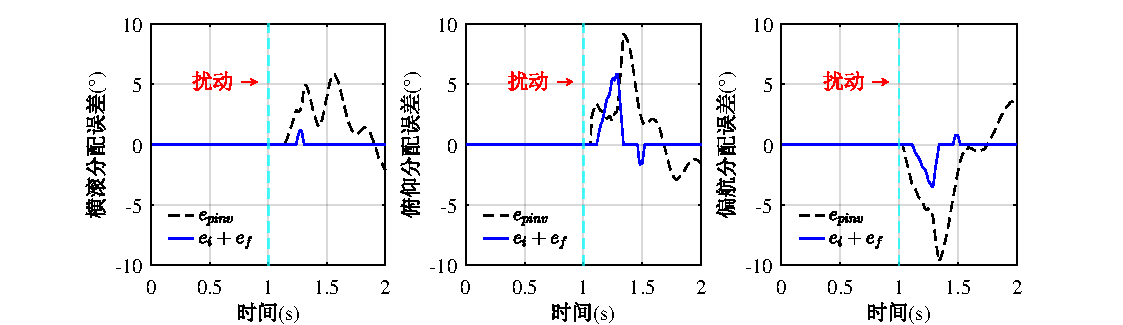
\includegraphics[scale=1]{Fig/优先级对比伪逆的分配误差飞行实验结果.pdf}
        \caption{\label{优先级对比伪逆的分配误差飞行实验结果}优先级对比伪逆的分配误差飞行实验结果}
        \end{minipage}
\end{figure}
\begin{figure}[htbp]
	\centering
	\begin{minipage}[c]{1\textwidth}
        \centering
        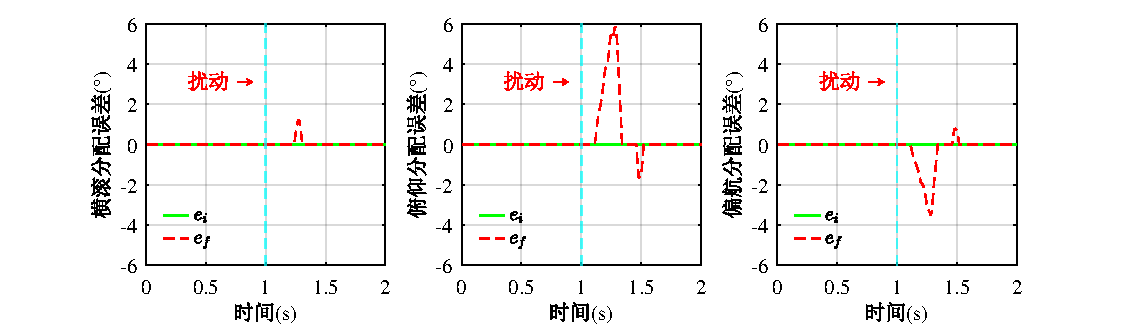
\includegraphics[scale=1]{Fig/优先级各分量的分配误差飞行实验结果.pdf}
        \caption{\label{优先级各分量的分配误差飞行实验结果}优先级各分量的分配误差飞行实验结果}
        \end{minipage}
\end{figure}

\section{本章小结}

本章围绕DFUAV的姿态控制问题展开研究,系统性地构建了基于INDI与优先级控制分配的理论框架及工程实现方案。首先介绍了INDI方法和控制分配理论以及两者在分层控制架构中的作用,然后通过姿态动力学模型简化降低了姿态动力学的非线性复杂度。进一步,提出了一种融合INDI架构与优先级控制分配的姿态控制策略,基于传感器的INDI方法对难以测得的力矩和外部扰动有较好的补偿能力,基于优先级控制分配可以最大程度保障虚拟控制输入中高优先级分量的可达性。最后通过一系列MATLAB仿真与实际飞行实验,证实了所提出的姿态控制方案相比于PID控制在扰动条件下仍能保持较小的跟踪误差,且控制分配误差也比传统的伪逆法更小。充分验证了所设计的姿态控制器的有效性,为下文的位置控制器设计奠定了基础。 % 第三章
% 自行根据需要添加章节。
...
\chapter{结\texorpdfstring{\quad}{}论}
本文主要是展示如何使用修改“祖传模板”得到的新模板,在使用时直接替换成自己的论文内容即可。

本模板难免有不足之处,主要是我本人的论文涉及的格式有限,有些地方没探索到自然就没去设置。比如附录,附录的图文并茂等等,我本人是没有研究的,这里仅仅做了一些初步的工作,不过对很多同学来说本模板是够用的。希望有能帮助到华工的同学们,有不足之处请多多理解,可以通过邮件联系我,我会尽量回复。
 % 结论
...
\printbibliography	% 参考文献著录
%%%%%%%%%%%%%%%%%%%此部分为附录环境代码,是比较笨的方法来适应论文撰写规范%%%%%%%%%%%%%%%%%%%%%%%%%%%%%%%%%%%%%%
%对只有一个附录,标题不编号比较美观。
%%%%%%%%%%%%%%%%%%%%%%%%%%%%%%%%%%%%%%%%%%%%%%%%%%%%%%%%%%%%%%%%%%%%%%%%%%%%%%%%%%%%%%%%%%%%%%%%%%%%%%%%%%%%
\setcounter{chapter}{1} %从1开始编号
\setcounter{section}{0}
\setcounter{equation}{0}
\setcounter{table}{0}   
\setcounter{figure}{0}
\chapter{附\texorpdfstring{\quad}{}录} %附录
%%%%%%%%%%%%%%%%%%%%%%%%%%%%%%%%%%%%%%%%%%%%%%%%%%%%%%%%%%%%%%%%%%%%%%%%%%%%%%%%%%%%%%%%%%%%%%%%%%%%%%%%
%%%%%%%%%%%%以下为用户代码,用于撰写您的论文%%%%%%%%%%%%%%%%%%%%%%%%%%%%%%%%%%%%%%%%%%%%%%%%%%%%%%%%%%%%%%


在论文撰写规范中,下面两段话让人费解:

\begin{enumerate}
	\item 	对需要收录于学位论文中但又不适合书写于正文中的附加数据、方案、资料、详细公式推导、计算机程序、统计表、注释等有特色的内容,可做为附录排写,序号采用“附录1”、“附录2”等。	
	\item	公式序号按章编排,如第一章第一个公式序号为“(1-1)”,附录2中的第一个公式为“(2-1)”等。
\end{enumerate}

论文撰写规范要求的附录和通常书籍上使用附录A、附录B等编号的不一样,容易和正文混淆。特殊的要求和代码的耦合,使我不得不使用比较笨的方法来设计附录部分的模板。

\section{测试测试测试}
\subsection{测试测试测试}
%
测试测试测试测试测试测试测试测试测试测试测试测试测试测试测试测试测试测试测试测试测试测试测试测试测试测试测试测试测试测试测试测试测试测试测试测试测试测试测试测试测试测试测试测试测试测试测试测试测试测试测试测试测试测试测试测试测试测试测试测试测试测试测试测试测试测试测试测试测试测试测试测试测试测试测试测试测试测试测试测试测试测试测试测试测试测试测试测试测试测试测试测试测试测试测试测试测试测试测试测试测试测试测试测试测试测试测试测试测试测试测试测试测试测试测试测试测试测试测试测试测试测试测试测试测试测试测试测试测试测试测试测试测试测试测试测试测试测试测试测试测试测试测试测试测试测试测试测试测试测试测试测试测试
\begin{align}
\left\{\begin{array}{l}
\dot{v}_{1}(t)=v_{2}(t) \\
\dot{v}_{2}(t)=R^{2}\left(-\zeta_{1}\left[v_{1}(t)-v_c(t)\right]^{\alpha}-\zeta_{2}\left[\dfrac{v_{2}(t)}{R}\right]^{\beta}\right)
\end{array}\right.	
\end{align}

\begin{align}
\left\{\begin{array}{l}
\dot{v}_{1}(t)=v_{2}(t) \\
\dot{v}_{2}(t)=R^{2}\left(-\zeta_{1}\left[v_{1}(t)-v_c(t)\right]^{\alpha}-\zeta_{2}\left[\dfrac{v_{2}(t)}{R}\right]^{\beta}\right)
\end{array}\right.	
\end{align}
\begin{figure}[htbp]
	\centering	
	\includegraphics[scale=1]{Fig/DFUAV_f31.png}
	\caption{\label{fig_case1}测试测试测试}
\end{figure}
\begin{figure}[htbp]
	\centering	
	\includegraphics[scale=1]{Fig/DFUAV_f31.png}
	\caption{\label{fig_case2}测试测试测试}
\end{figure}
\begin{table}
	\caption{\label{DF_para1}测试测试测试}
	\centering{}%
	\small 
	\begin{tabular}{cccccc}
		\hline 
		参数符号 & 数值&参数符号 & 数值&参数符号 & 数值\tabularnewline
		\hline 
		$ A_x,A_y,A_z $  & $ 0.04082\,\text{m}^2 $ &$ \rho $        &$1.225\,\text{kg}/\text{m}^3$&$ I_b $           & $ 0.000029 $               \tabularnewline
		$ k_{\varpi} $   & $1.13342 \times 10^{-6}$& $ d_{\varpi} $ & $1.13342 \times 10^{-7}$ 	  &$k_{\delta} $     & $ 0.01495 $ 			      \tabularnewline
		$C_{D,x},C_{D,y}$& $ 0.43213 $             &$ C_{D,z} $     & $ 0.13421 $             	  &	$ q_a $ 	     & $ 1.49 $ 				  \tabularnewline
		$ l_{a} $        & $ -0.1121\,\text{m} $   & $ d_{ds} $     & $ 0.01495 $			  	  &$ d_{af} $        & $ 0.01495 $    			  \tabularnewline
		$ R $            & $ 0.11\,\text{m} $      &$ b $           & $ 2 $       			   	  &$ S $ 			 & $ 0.04082\,\text{m}^2 $    \tabularnewline
		$C_{l_{\alpha}}$ & $ 2.212\,/\text{rad} $  &$C_{l, \max } $ & $ 1.05 $ 				   	  &$ C_{l, \min } $  & $ -1.05 $ 				  \tabularnewline
		$ l_2 $          & $ 0.06647\,\text{m} $   &$ l_1 $         & $ 0.17078\,\text{m} $    	  &	$ m $ 		     & $ 1.53\,\text{kg} $ 		  \tabularnewline
		$ C_{d, o } $    & $ 0.9 $                 &$ C_{d, g } $   & $ 0.9 $					  &$ C_{duct} $      & $ 0.78497 $	 			  \tabularnewline
		$ I_x $          & $ 0.02548 $ 			   &$ I_y $         & $ 0.02550 $                 &$ I_z $			 & $ 0.00562 $ 				  \tabularnewline
		\hline 
	\end{tabular}	
\end{table}

\begin{table}
	\caption{\label{TDF_para2}测试测试测试}
	\centering{}%
	\small 
	%	\resizebox{\textwidth}{!}{
	\begin{tabular}{cccccc}
		\hline 
		参数符号 & 数值&参数符号 & 数值&参数符号 & 数值\tabularnewline
		\hline 
		$ I_x $ & $ 054593 $ &$ I_y $ & $ 0.017045 $& $ I_z$ & $ 0.049226 $ \tabularnewline
		$ l_{1} $ & $ 0.0808\,\text{m} $&$ l_{2} $ & $ 0.175\,\text{m} $ &$ l_3 $ & $ 0.06647\,\text{m} $ \tabularnewline 
		$ l_4 $ & $ 0.2415\,\text{m} $ &$ l_5 $ & $ 0.1085\,\text{m} $& $ m $ & $ 3.7\,\text{kg} $ \tabularnewline
		\hline 
	\end{tabular}	%}
\end{table}

\section{测试测试测试}
\subsection{测试测试测试}
%
测试测试测试测试测试测试测试测试测试测试测试测试测试测试测试测试测试测试测试测试测试测试测试测试测试测试测试测试测试测试测试测试测试测试测试测试测试测试测试测试测试测试测试测试测试测试测试测试测试测试测试测试测试测试测试测试测试测试测试测试测试测试测试测试测试测试测试测试测试测试测试测试测试测试测试测试测试测试测试测试测试测试测试测试测试测试测试测试测试测试测试测试测试测试测试测试测试测试测试测试测试测试


 % 附录
\chapter{攻读博士/硕士学位期间取得的研究成果} %博士/硕士记得选其一
\pubfont % 论文撰写规范里,这章是5号宋体,\pubfont 设置字号为5号了。但其实很多论文用小四号也OK。
一、已发表(包括已接受待发表)的论文,以及已投稿、或已成文打算投稿、或拟成文投稿的论文情况\underline{\textbf{(只填写与学位论文内容相关的部分):}}
\begin{table}
	\centering{}%
	\pubfont 
	\begin{longtable}{|>{\centering}m{0.5cm}|m{1.8cm}|>{\centering}m{2.8cm}|>{\centering}m{2.5cm}|>{\centering}m{2.2cm}|>{\centering}m{2.cm}|>{\centering}m{1cm}|}
		\hline 
		\textbf{序号} & \textbf{作者(全体作者,按顺序排列)} & \textbf{题 目} 						   & \textbf{发表或投稿刊物名称、级别} & \textbf{发表的卷期、年月、页码} & \textbf{与学位论文哪一部分(章、节)相关} &\textbf{被索引收录情况}\tabularnewline
		\hline 
		1    & 					  &  &  &  &  &  \tabularnewline
		\hline 
		2	 & 							&  	 &   &  &  & \tabularnewline
		\hline 
	\end{longtable}
\end{table}

注:在“发表的卷期、年月、页码”栏:

1.如果论文已发表,请填写发表的卷期、年月、页码;

2.如果论文已被接受,填写将要发表的卷期、年月;

3.以上都不是,请据实填写“已投稿”,“拟投稿”。

不够请另加页。

二、与学位内容相关的其它成果(包括专利、著作、获奖项目等)



%注:这部分一言难尽,我努力了很久都没有把这个表做好。感觉学校给的这个表的模板非常反人类。看国外大学的博士论文,那种像参考文献著录信息那样一行一行的,比较美观。而这个框框很难放文字进去。

\normalsize % \normalsize可以将下文调回和正文一样的字号,这个随个人喜好。注释掉的话,致谢就就跟随《攻读博士/硕士学位期间取得的研究成果》的字号。 % 成果
\chapter{致\texorpdfstring{\quad}{}谢}
%把下面文字替换
\begin{center}
这次你离开了没有像以前那样说再见,再见也他妈的只是再见 
~\\
我们之间从来没有想象的那么接近,只是两棵树的距离 
~\\
你是否还记得山阴路我八楼的房间,房间里唱歌的日日夜夜 
~\\
那么热的夏天你看着外面,看着你在消逝的容颜 
~\\
我多么想念你走在我身边的样子,想起来我的爱就不能停止 
~\\
南京的雨不停地下不停地下,就像你沉默的委屈 
~\\
一转眼,我们的城市又到了夏天,对面走来的人都眯着眼 
~\\
人们不敢说话不敢停下脚步,因为心动常常带来危险 
~\\
我多么想念你走在我身边的样子,想起来我的爱就不能停止 
~\\
南京的雨不停地下不停地下,有些人却注定要相遇 
~\\
你是一片光荣的叶子,落在我卑贱的心 
~\\
像往常一样我为自己生气并且歌唱 
~\\
那么乏力,爱也吹不动的叶子 
\end{center}
%把上面文字替换

~\\

\begin{minipage}[t]{0.945\textwidth}%
	\begin{flushright}
		作者姓名\\
%		\today\\	% 自动时间
		2020年7月10日\\	%固定时间
		于华南理工大学
		\par\end{flushright}
\end{minipage}

 % 致谢
\end{lstlisting}
其中$\%$之后的内容为注释,...表示省略其他代码,仅保留论文内容主体部分。\textbackslash{}include\{xxx\}指令用于包含xxx.tex文件的内容,各章节的内容主要在xxx.tex中保存。在\textbackslash{}documentclass 和\textbackslash{}begin\{document\} 之间的位置称为导言区。在导言区中一般会使用\textbackslash{}usepackage 调用宏包,以及会进行对文档的全局设置。本模板的导言区除调用所需的宏包外,还进行了页眉页脚的设置。有的模板会把所有调用宏包的指令放到一个.sty宏包文件中,页面的设置放在文档类文件.cls文件中。因本人时间有限,就不做整理,欢迎有志之士加入完善。使用本模板并不需要了解导言区的指令,在需要时额外添加即可(要注意宏包冲突)。特别地,\textbackslash{}includeonly\{xxx\}指令用于使文档仅编译xxx.tex文件的内容,这就是分章节包含(include)的好处,可大大减少编译时间。

将封面打印保存为 thesis\_cover.pdf 文件,硕士使用master\_cover.docx ,博士使用 doctor\_cover.doc 。如果有更新版本的封面,可自行替换。文档类默认是博士论文,下面指令将控制添加封面与否:
\begin{lstlisting}
\documentclass[unicode,master,pdfcover]{scutthesis}	% 使用pdf文件封面的 硕士模板
\documentclass[unicode,master]{scutthesis}	% 不使用pdf文件封面的 硕士模板
\documentclass[unicode,pdfcover]{scutthesis}	% 使用pdf文件封面的博士模板
\documentclass[unicode]{scutthesis}	% 不使用pdf文件封面的博士模板
\end{lstlisting}
不使用thesis\_cover.pdf 文件指定的封面时,将使用草稿封面。草稿封面也可以减少编译时间,因此可以在最终提交论文时再使用论文封面。草稿封面用以下指令设置:
\begin{lstlisting}
%%%%%%%%%%%%%草稿封面设置%%%%%%%%%%%%%	
\title{LaTeX模板}	
\author{作者姓名}	
\supervisor{指导教师:xxx\ 教授}	
\institute{华南理工大学}	
\date{2020年5月20日}
%%%%%%%%%%%%%%%%%%%%%%%%%%%%%%%%%%%%%
\end{lstlisting}
\section{章节文件}
chapter文件夹的章节文件如chapter0x.tex等,其内容由\textbackslash{}chapter\{章名\}开头。新建一章可新建一个文件并由\textbackslash{}chapter\{新建章名\}开头填写内容即可。节及小节分别用\textbackslash{}section\{新建节名\}、\textbackslash{}subsection\{新建小节名\}命令。

正文的的书写和txt文本文件的书写类似。\LaTeX{} 源代码中,空格键和Tab键输入的空白字符视为“空格”。连续的若干个空白字符视为一个空格。一行开头的空格忽略不计。行末的回车视为一个空格;但连续两个回车,也就是空行,会将文字分段。多个空行被视为一个空行。也可以在行末使用\textbackslash{}par 命令分段。在本模板中,英文之间的空格被保留,中文之间的空格被忽略。特别地,摘要,附录,结论等两个字的大纲级别为章的章名,中间使用空格隔开。对此论文撰写规范并没有明文要求,只是为了美观。也可以全部不加空格。一般情况下,在文本文字中添加空格使用\textbackslash{}quad命令,但由于文献\parencite{_d}所述原因,直接使用\textbackslash{}quad命令会报警,因而使用\textbackslash{}texorpdfstring\{\textbackslash{}quad\}\{\},其中最后一个\{\}里面可以加一个空格,不影响使用。目录二字之间添加空格在scutthesis.cls文件317行设置。

正文本环境中使用公式,即行内公式,需要用两个\$包围,如源码:\$a+b=c\$ 显示为$a+b=c$。使用其他字符可自行百度或阅读参考文献。再次提醒,使用\LaTeX{}撰写论文不需要研究其原理,在达到某种效果(图文显示、公式显示效果)时百度或查书寻找其代码即可。

综上,论文撰写只需要将自己的文本(包含行内公式)放到相应的章节处,并添加行间公式、图表环境并填写图表即可。行间公式、图表将在下一章介绍。

